\chapter[Machine learning for CWs]{\label{machine} Machine learning for continuous wave searches}
%%%%%%%%%%
%%%%%%%%%%
%\epigraph{Everyone Knows That When You Make An Assumption, You Make An A** Out Of 'U' And 'Umption.}{ --- \textit{Samuel Jackson (Mitch Henessey)}, The Long Kiss Goodnight}

%--------------------------
% Introduce machine learning
%----------------------------

`Machine learning' is a term which has been around since the 1950s, and is a subset of what is known as `artificial intelligence'.
This is a field which aims to use computers to learn information without being given explicit instructions.
With the increase in available computing power in recent years along with the easier access to large data-sets, machine learning has become a much more accessible technique.
One of the techniques in particular is a method known as deep learning which uses deep neural networks.
These have been used extensively in classification problems as well as many others.
Neural networks wave a large range of applications, and have gained increasing popularity for use in \gls{GW} data analysis problems.

%------------------------
%Overview of what is chapter is
%--------------------------
This chapter aims to give an overview of neural networks, specifically \glspl{CNN} and their application to a \gls{CW} search. 
The majority of this section is written in a paper which is yet to be published, however, is aimed to be submitted soon.
The differences are, Sec.~\ref{machine:nn}, \ref{machine:cnn} and \ref{machine:training} which describe the operation of neural networks have more detail in this thesis than in the paper draft. 
Sec.\ref{machine:results:sens_size} is additional material which is currently not included in the paper draft.


%%%%%%%%%%%%
%%%%%%%%%%%%%%%
\section{\label{machine:intro} Introduction}
%%%%%%%%%%%%
%%%%%%%%%%%%%

% Intro to GWs and CW
%
Gravitational wave detectors such as \gls{LIGO}~\cite{abbott2009LIGOLaser,aasi2015AdvancedLIGO} and VIRGO
\cite{acernese2015AdvancedVirgo,acernese2008StatusVirgo} search for a number of different targets. 
Some targets such as \glspl{CBC} have been observed ~\cite{abbott2017GW170817Observation,abbott2017GW170814ThreeDetector,abbott2016ObservationGravitational},
however, other primary sources such as \glspl{CW} are yet to be observed.
\glspl{CW} are well modelled quasi-sinusoidal signals with a
duration much longer than observing times of detectors.
The source of these signals is thought to be rapidly rotating neutron stars which can emit \gls{GW} if there is some asymmetry around its rotation axis. 
This can be caused by various mechanisms as described in ~\cite{prix2009GravitationalWaves}. 
These signals have small amplitude, which if detected will be below the noise \gls{PSD} of the detector.
Therefore, sensitive search algorithms are needed to find the signals. 
These algorithms generally fall into three categories: Targeted,
directed, and all-sky searches, listed in order of how much is known a priori
about the source from \gls{EM} observations. 

% describe the different general types of CW search
%
In targeted searches the sky position, frequency, and its derivatives are
assumed to be well known, in directed searches only the sky position is
known and in all-sky searches the sky position and frequency of the source is unknown.
The most sensitive of these are targeted searches which use coherent matched
filtering~\cite{dupuis2005BayesianEstimation,schutz1998DataAnalysis}. These use
template waveforms which are generated using the information already known about the
source, then correlated this with the data. Directed and all-sky searches have
a much broader parameter space to search, therefore, many templates are needed
to sufficiently cover the parameter space. Using the coherent matched filter
for broader parameter space searches becomes unfeasible due to the amount of
computing time that is needed. This led to the development of semi-coherent
searches where the data is divided up into smaller segments which can be analysed
separately and then the results can be recombined incoherently using various
methods~\cite{abbott2019AllskySearch,creighton2000SearchingPeriodic}. Semi-coherent
searches result in a trade off between sensitivity and computing time.

% Introduce SOAP and explain the line artefact problem
%
The analysis here is presented mainly as an addition to an existing
semi-coherent search algorithm titled SOAP~\cite{bayley2019SOAPGeneralised}.
This is a fast and largely un-modelled search which finds tracks of
high \gls{FFT} power in time-frequency spectrograms. 
When applied to multiple detectors using a line-aware statistic, SOAP looks for frequency bins which have both a high power and are similar in each detector. 
This means that  at a given frequency at a given time, SOAP will penalise frequencies where the \gls{FFT} power is largely different in each detector.  
The algorithmic details summarised in Sec.~\ref{soap}. 

% instumental lines and how the affect SOAP
%

One effect which limits the sensitivity of SOAP and many other
\gls{GW} searches is noise artefacts known as `instrumental lines'. These can be anything
from long duration fixed frequency or wandering lines to shorter duration fixed frequency transients. 
There are certain types of instrumental line which the SOAP search can struggle to distinguish from an astrophysical signal even with the development of a
`line aware' statistic in~\cite{bayley2019SOAPGeneralised}. Currently the
method used to reduce the effect of these lines is to manually look at the SOAP
output and the spectrograms for each sub-band to determine whether the sub-band
is contaminated by instrumental effects. This process is slow, requires a
lot of human input and is subject to human error. When the search runs over
a larger bandwidth, it will no longer be practical to look
through all bands. 

% Convolutional neural networks
%

We aim to automate how the search deals with instrumental lines by using \glspl{CNN}.
These have been used extensively in image classification and we explain this in
more detail in Sec.~\ref{machine:cnn}. \glspl{CNN}
have already been shown to detect gravitational wave signals from \glspl{CBC}
in~\cite{gabbard2018MatchingMatched,george2018DeepLearning,gebhard2019ConvolutionalNeural}
and other deep learning techniques have been used in searching for \gls{CW}
signals in~\cite{dreissigacker2019DeeplearningContinuous}. 

% structure of the paper
%
In Sec.\ref{cnn:soap} we will summarise the basics of how the SOAP search works. In
Sec.~\ref{machine:nn}, \ref{machine:cnn} and \ref{machine:training} we explain how \glspl{CNN} operate and how they are trained. Sec.~\ref{machine:cw} will describe how this is applied to an \gls{CW} search. 
This includes the structure of the \gls{CNN} in Sec.~\ref{machine:cw:structure} and the entire search from raw data to results in Sec.~\ref{machine:pipeline}. Finally in Sec.~\ref{machine:results} we
show the results from this search and compare to similar analyses. 

%%%%%%%%%%%%%%%%%%%%%%%%%%%
%%%%%%%%%%%%%%%%%%%%%%%%%%
\section{\label{cnn:soap} SOAP}
%%%%%%%%%%%%%%%%%%%%%%%%%%
%%%%%%%%%%%%%%%%%%%%%%%%%%%

% introduce SOAP and show example of outputs
%
In Chapter \ref{soap} we introduced the SOAP algorithm. 
To recap SOAP~\cite{bayley2019SOAPGeneralised} is an un-modelled search for long
duration signals which is based on the Viterbi
algorithm~\cite{viterbi1967ErrorBounds}. In its most simple form SOAP
analyses a spectrogram to find the time-frequency track which gives the highest
sum of \gls{FFT} power. If a signal is present and sufficiently loud then this
is the track which is most likely to come from some signal.
In~\cite{bayley2019SOAPGeneralised} the algorithm has been expanded to
search through multiple detectors as well as including a statistic to penalise
artefacts in the data from the instrument as opposed to from an astrophysical
source. 

% refer to the figure showing the Viterbi track for S6
%
Fig.~\ref{soap:viterbiplot} shows an example of the spectrogram data which is
searched through and the outputs of SOAP; the three main output components are
the frequency track, the Viterbi statistic and the Viterbi map.

\begin{figure}[ht]
	%\centering
	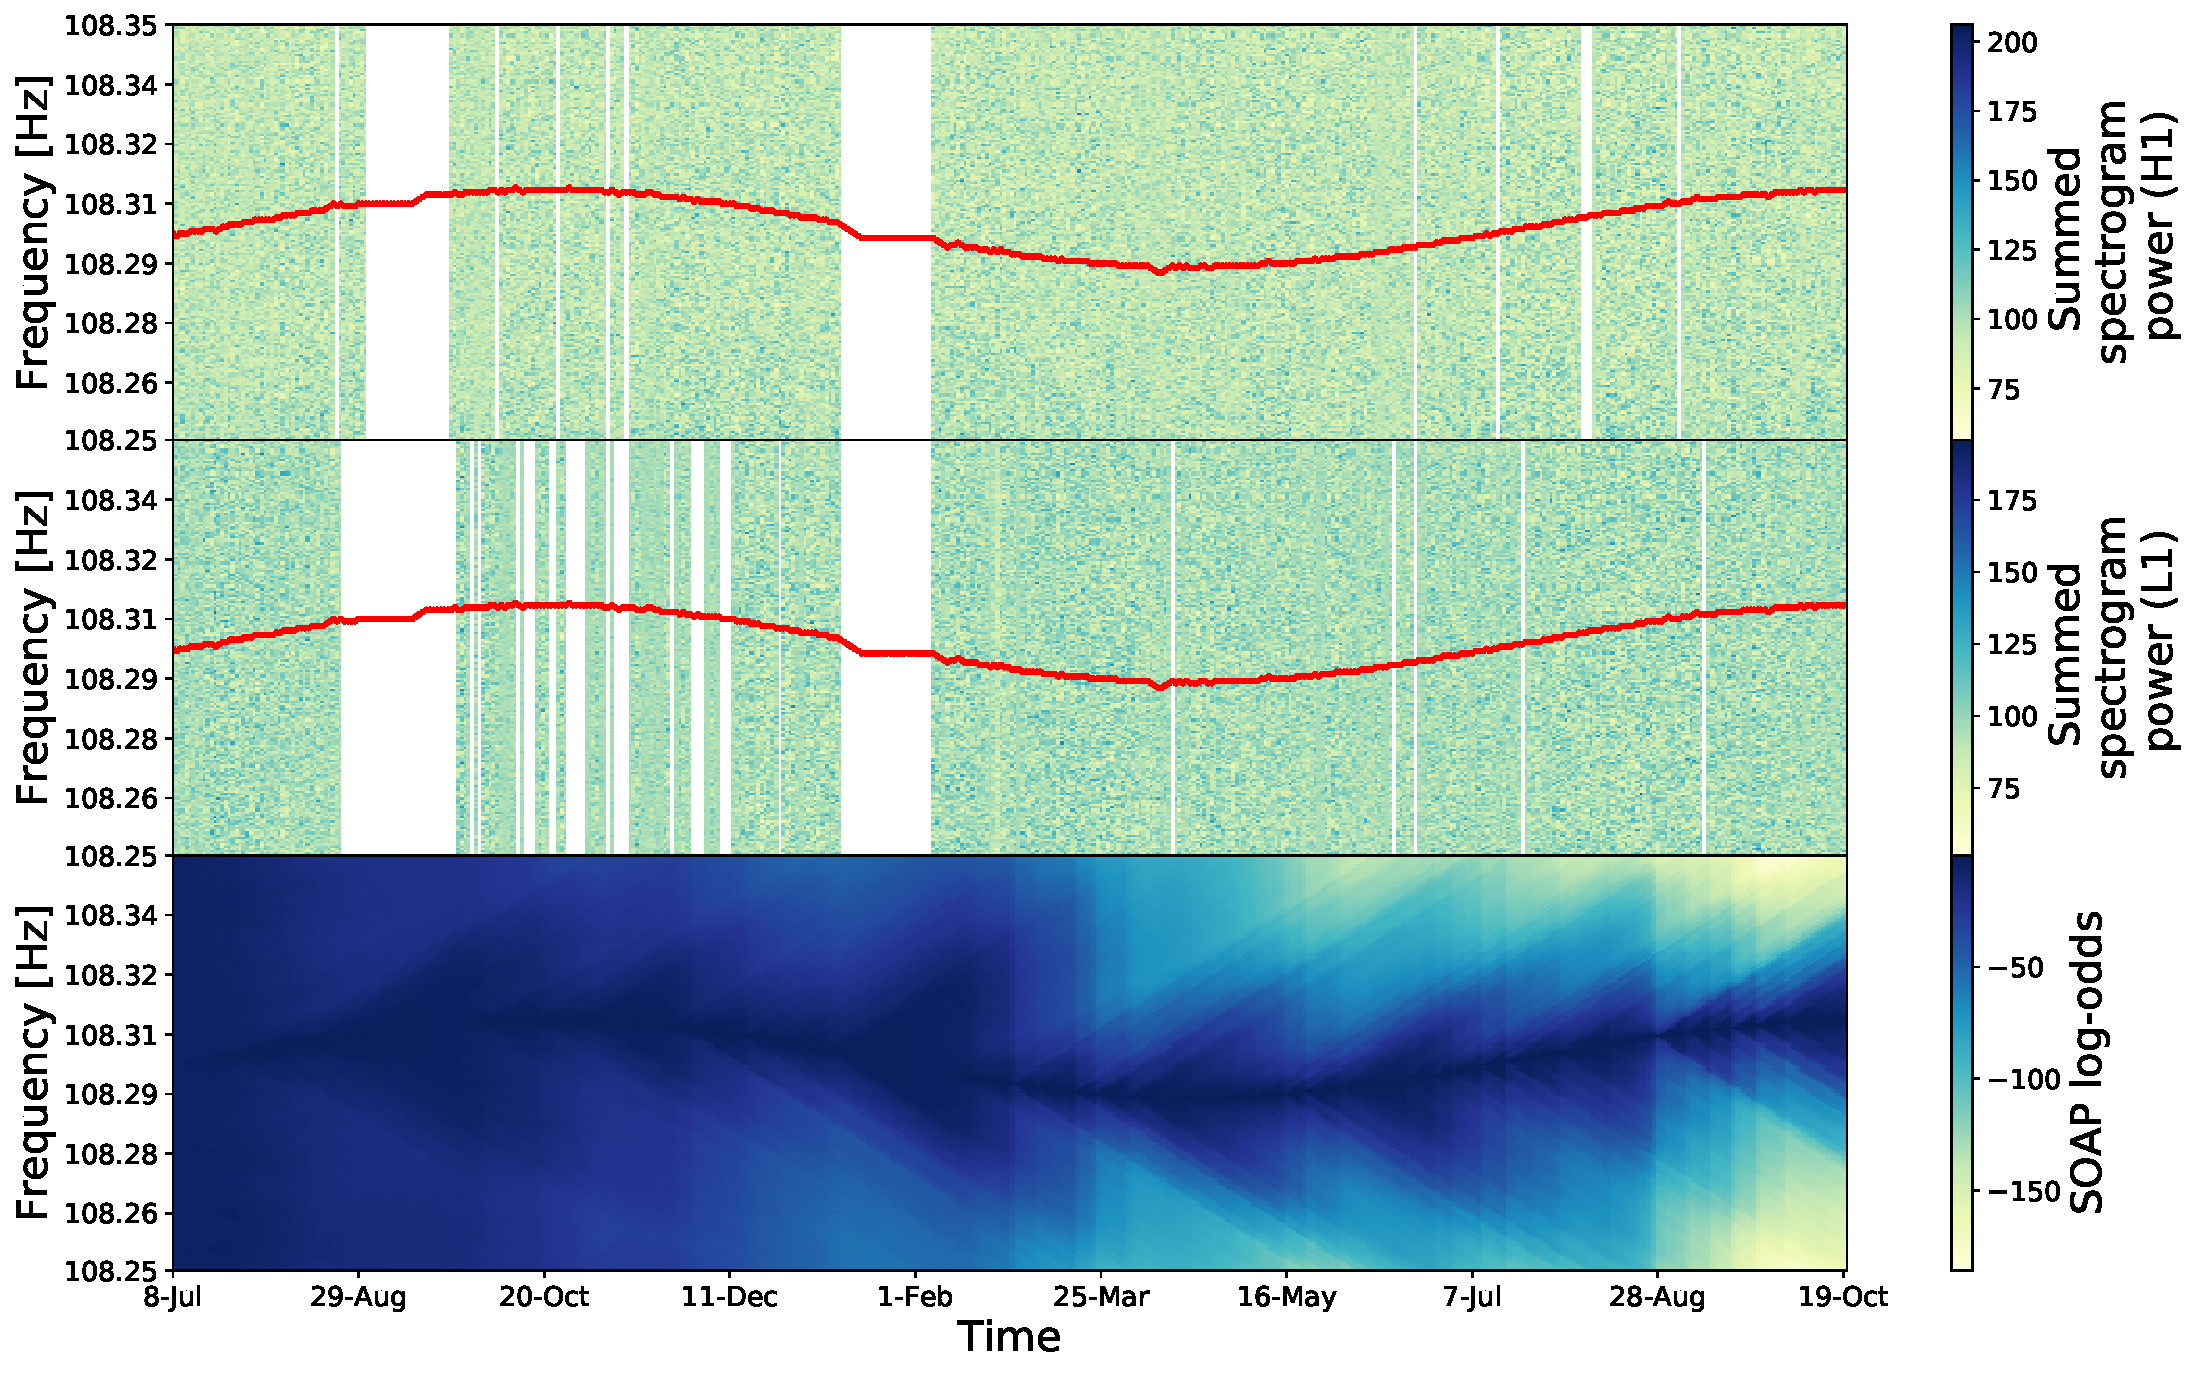
\includegraphics[scale=0.43]{C4_cnn/two_vit_example.pdf}
	%
	\caption[Example SOAP output from H1 and L1 input spectrograms. ]{\label{soap:viterbiplot} This plot shows the inputs and outputs of the
		SOAP search. The top two panels are time-frequency spectrograms which have been pre-processed as described in Sec.~\ref{machine:pipeline}. This
		data is a 0.1 Hz wide frequency band from the S6 observing run \cite{} \joe{reference} which includes a string simulated \gls{CW} signal. The white areas in the spectrograms are gaps in data when the detector was not operating. These both have the
		optimal track found by SOAP overlaid. The bottom panel shows the normalised Viterbi map, the intensity of a
		pixel in this image relates to the log-probability that a track ends in and
		particular frequency bin at a given time.}
	%
\end{figure}

% describe the main data products from the search
%
\begin{description} 
	%
	\item [Viterbi track] The Viterbi track is the most probable track through time-frequency data given a choice of statistic. 
	%
	\item [Viterbi statistic] The Viterbi statistic is the sum of the individual statistics along the Viterbi track. In the analysis that follows, the `line-aware' Viterbi statistic is used. 
	This is the sum of the log-odds ratios, $p_{\rm signal}/(p_{\rm line} + p_{\rm noise})$ along the track. This is defined in more detail in \cite{bayley2019SOAPGeneralised}
	%
	\item [Viterbi map]
	The Viterbi map value of the Viterbi statistic for every time-frequency bin in the spectrogram. 
	This represents the most probable track which ends in any time-frequency bin.
	In the Viterbi maps, each time slice is normalised individually, i.e., each
	vertical slice has been normalised such that the sum of their exponentiated
	values is equal to 1. This way each pixel in the image can be interpreted as a
	value related to the log-probability that there is a signal in the bin at that
	time.
	%
\end{description}

% Mention line aware statistic
%
To determine whether an simulated astrophysical signal has been detected,
in~\cite{bayley2019SOAPGeneralised} we used the Viterbi `line aware' statistic alone described above.  
The `line-aware' statistic reduced the affect of instrumental lines on the analysis, however the `line-aware' statistic is still contaminated by certain types of line.
For example, the statistic is affected by broad wandering lines as they offer high power tracks in both detectors.
To reduce the effect of these instrumental lines, we looked through the spectrograms and
Viterbi maps of individual bands by eye as in Fig.~\ref{soap:viterbiplot}.
Bands which appeared to be contaminated were then removed from the search.

% what was different in this analysis
%
In this search the spectrograms and the Viterbi map contained extra information
over the Viterbi statistic. 
We aim to utilise this in addition to the Viterbi statistic to replace the process of removing contaminated bands `by eye' and therefore automating the search. 
A useful tool which can be used to classify this extra information is convolutional neural networks. 

%%%%%%%%%%%
%%%%%%%%%%%
\section{\label{machine:nn}Neural networks}
%%%%%%%%%%%
%%%%%%%%%%%

\joe{add some references in this section}
Throughout this section I will summarise one machine learning technique known as a neural network. 
Neural networks, as the name may suggest, were developed as a way for a computer to mimic neurons in the brain.
To understand why this would be useful, one can try to design an algorithm to identify hand written digits.
This seems like a simple task as a brain can complete with ease. 
However, writing a traditional algorithm to perform this same task is very difficult. 
The algorithm would have to identify a particular shape which has a huge amount of variation.
Neural networks offer a way to deal with this problem as they can be trained on large datasets, similar to how a human brain is `trained'. 
In the lifetime of a brain, many examples of different hand written digits are seen. 
For each new example the brain `updates' itself based on the new version of the observed digit. 
This process is replicated in a neural network where the algorithm can be updated for each example, with the goal of correctly identifying a digit.
A neural network has many parameters which can be modified or `trained', it is these parameters which are updated after each new example of a digit. 
These parameters are grouped into objects called neurons, many combinations of neurons can then be used to build a neural network.

%%%%%%%%%
%%%%%%%%%
\subsection{\label{machine:nn:neuron}Neurons}
%%%%%%%%%
%%%%%%%%%

Neurons are the building blocks of any neural network.
They perform simple operations on any number of input values and then output a single value.
The output $o$ of a neuron is defined by the equation

\begin{equation}
    o = f\left(b + \sum_{i=1}^{N} w_i x_i  \right),
    \label{machine:nn:neuron:equation}
\end{equation}

where $b$ is the bias, $x_i$ is an input value with a corresponding weight $w_i$, $f$ is the activation function, $o$ is the output and $N$ is the number of inputs.
Here the inputs $\mathbf{x}$ represents either the data which is input, in the example above this is the pixels in the digits image, or the output of another neuron.
The weights $\mathbf{w}$ then represent the importance of each data point to this neuron. 
The bias $b$ is then just an extra factor which can shift the data by a fixed value.
The activation function $f$ is then a function which can have many forms, in the simplest case in a neuron known as a `perceptron', it provides a cut where any value above a given threshold is 1 and any below is 0, this will be explained in more detail in Sec.~\ref{machine:nn:activation}. 

\begin{figure}[ht]
    \centering
    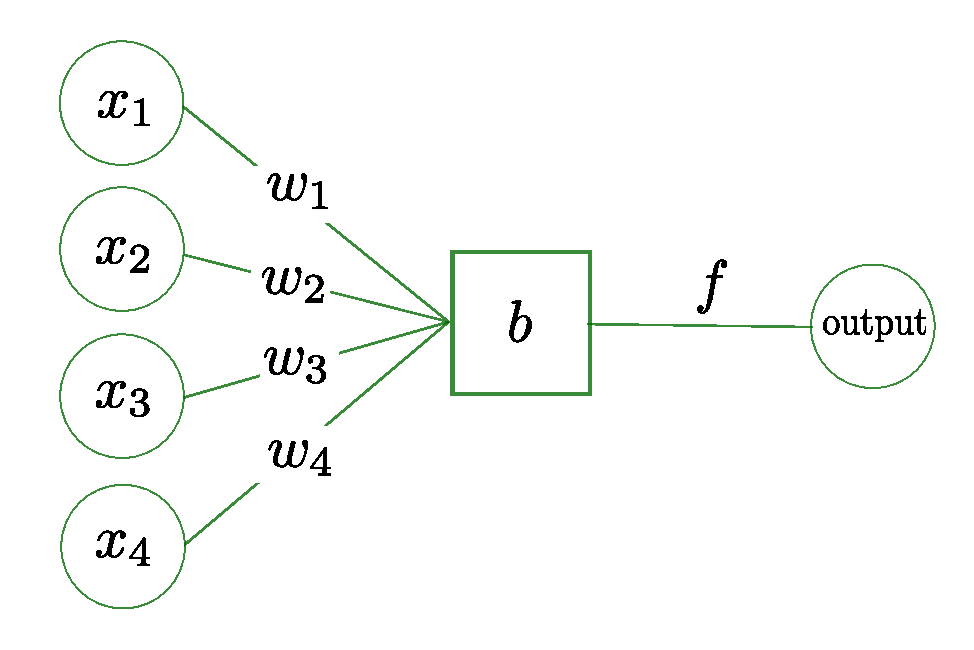
\includegraphics[width=0.6\columnwidth]{C4_cnn/neuron.pdf}
    \caption[Basic neuron]{Basic neuron showing the four input parameters $x_n$ and their corresponding weights $w_n$. These are multiplied and summed as in Eq.~\ref{machine:nn:neuron:equation}. A bias $b$ is added and this value is passed through and activation function $f$ to the output.}
    \label{machine:nn:neuron:plot}
\end{figure}

In the example in Fig.~\ref{machine:nn:neuron:plot} I have shows a neuron which has 4 input variables, or 4 input data points. 
When a network is trained the weights and the bias are updated to better represent the input data.
This training procedure is explained in more detail in Sec.~\ref{machine:nn:training}.
Many neurons are then used in combination with each other to develop a neural network which can be applied to more complex problems.

%%%%%%%%%%%%%%%%%%%%
\subsection{\label{machine:nn:structure}Network structure}
%%%%%%%%%%%%%%%%%%%%

The structure of a neural network is defined by the user and there is no set way to design a network.
However, the general layout of a neural network is defined by structures called layers, sometimes known as fully connected layers. 
These are rows of $N$ neurons which all take the same input such that there is $N$ output values.
An example of a simple neural network is shown in Fig.~\ref{machine:nn:structure:plot}.
The first layer is the input layer, this is just the data points from an input example.
In the example of hand drawn digits, this would be the pixels from the image of the digit.
The final layer represents the information that you intend the network to extract from the input data. 
In the hand drawn digit example, this could have 10 output neurons corresponding to each digit 0-9. 
Each of these outputs is then a value which is related to the probability of that digit being present in the image.  

When designing a network, the user will have a defined input layer size from the data and a desired number of output neurons which represents, for a classification example, the number of output classes. 
The number of hidden layers and the number of neurons in those hidden layers can be arbitrarily changed. 
In general if the data contains more complex information the size or complexity of the network will need to be increased for it to be able to extract the information. 

\begin{figure}[ht]
    \centering
    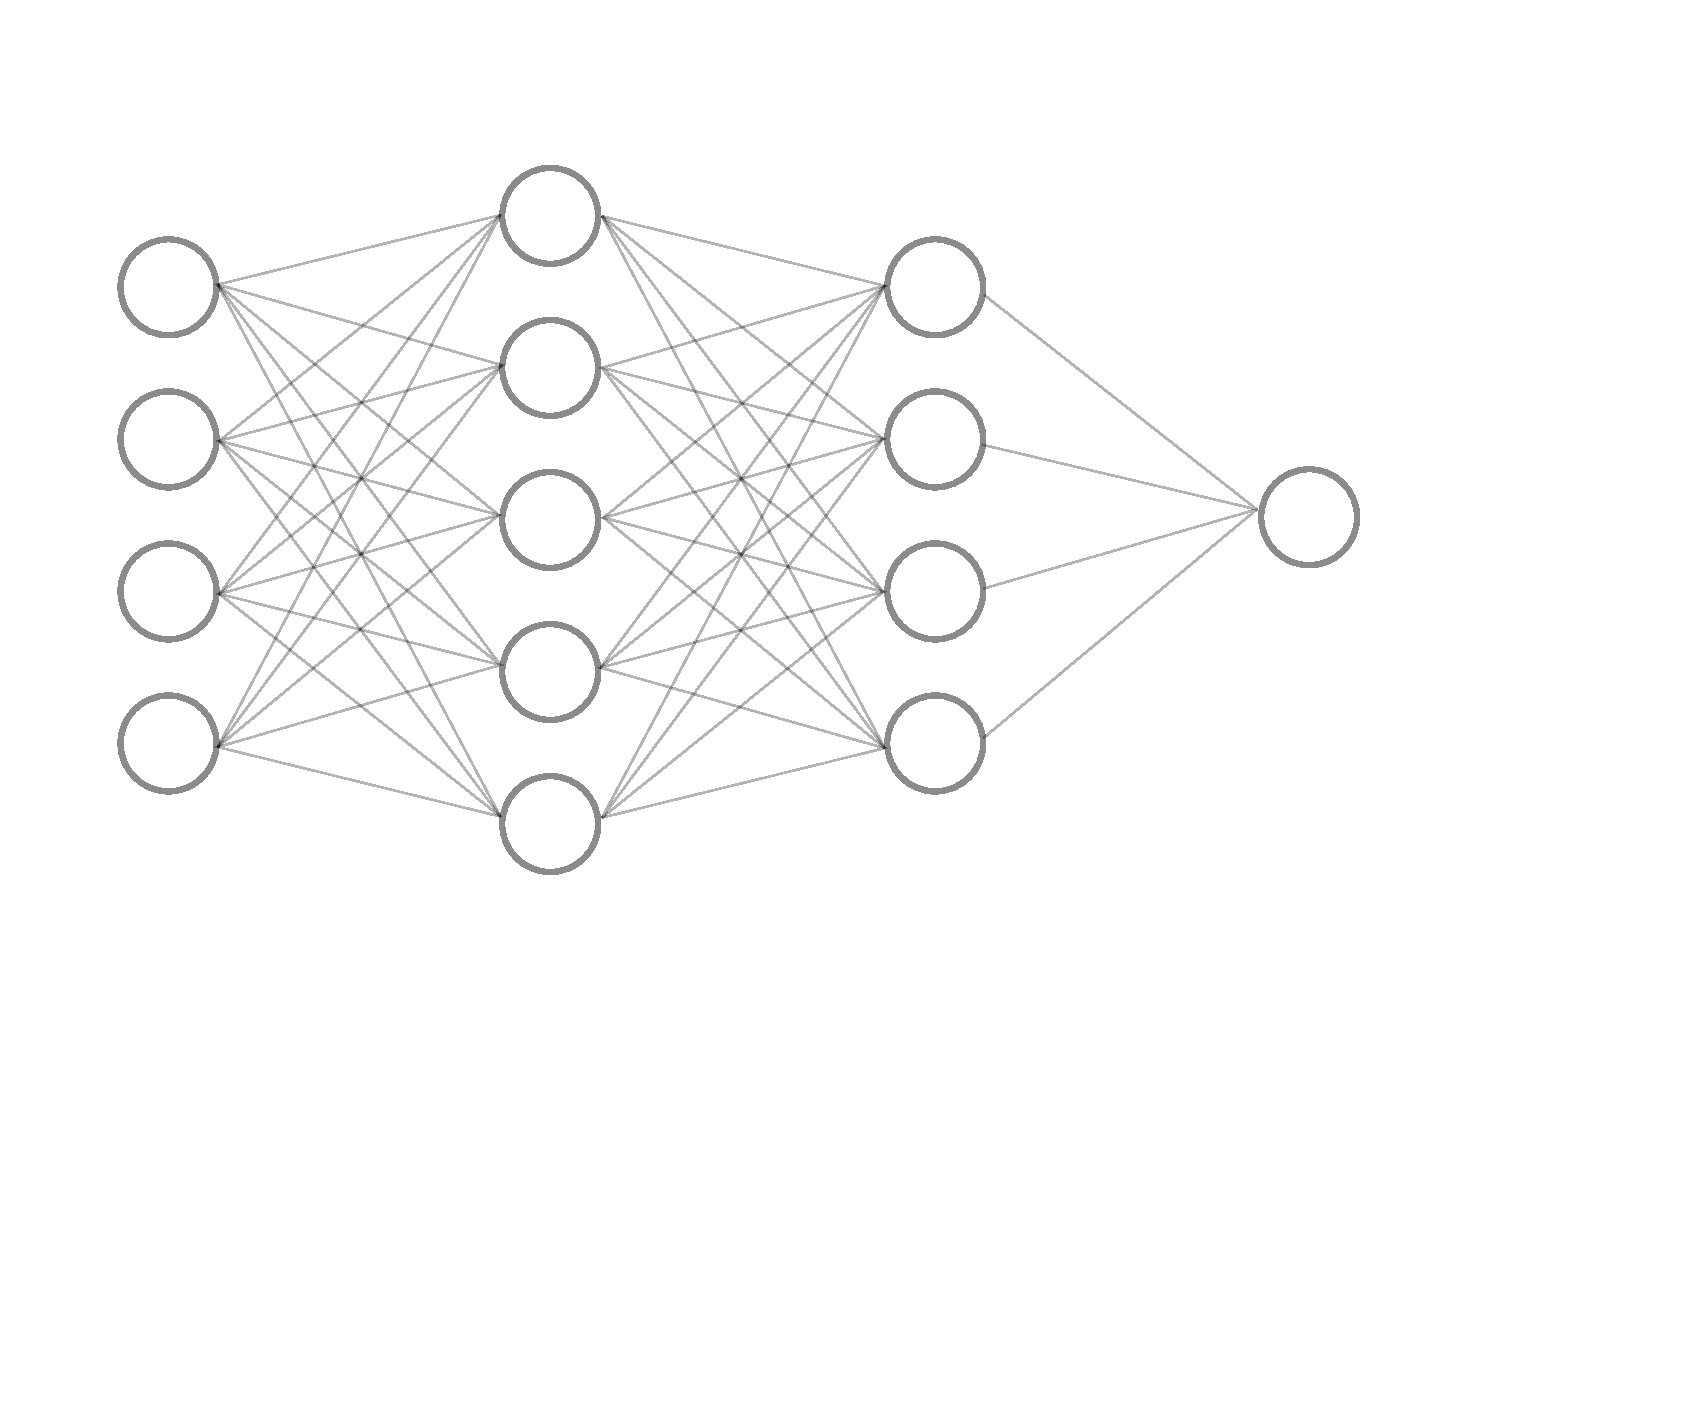
\includegraphics[width=\columnwidth]{C4_cnn/simple_network.pdf}
    \caption[Example structure of a neural network.]{A neural network is structured with layers. Each of the circles in these layers are neurons as described in Sec.~\ref{machine:nn:neuron} and Fig.~\ref{machine:nn:neuron:plot}. The networks contain an input layer which is usually the data which you would like to analyse. Then this passes to a number of `hidden' layers, in the above diagram there are two. Hidden layers are just layers which exist between the input and the output. The output layer is then the desired output, above I have chosen a single neuron as output. This is such that the network could classify the input to a value between 0 and 1. Every neuron in a layer is connected to the output of all neurons in the previous layer.}
    \label{machine:nn:structure:plot}
\end{figure}


%%%%%%%%%%%%%%%%%
\subsection{\label{machine:nn:activation}Activation functions}
%%%%%%%%%%%%%%%%%

The activation function transforms the sum of the data and weights as in Eq.~\ref{machine:nn:neuron:equation}. 
The most simple activation function is to set a threshold where for any number above this the output is 1 otherwise the output is zero. However, this type of activation known as a perceptron does not always perform well in neural networks.
Activations functions are generally non-linear, this reflects the non-linearity of real world problems and allows networks to learn that. 
A linear activation function means that any number of layers in a network is equivalent to a single layer network.
Another property which is desired in activation function is that it is continuously differentiable. This is to allow algorithms such as gradient descent to optimise the network \citep{nwankpa2018ActivationFunctions}. 
There are many choices when defining this in the network, some of the available options are shown in Fig.~\ref{machine:nn:activation:plot} \citep{nwankpa2018ActivationFunctions}.
One of the more commonly used activation function is the LeakyRELU function, this is explained in more detail in \citep{maas2013RectifierNonlinearities}.
In the work that follows we use the LeakyRELU function and the sigmoid function.
The sigmoid function is used on the output such that values are constrained between 0 and 1, the LeakyRELU is used everywhere else. 


\begin{figure}[ht]
	\centering
	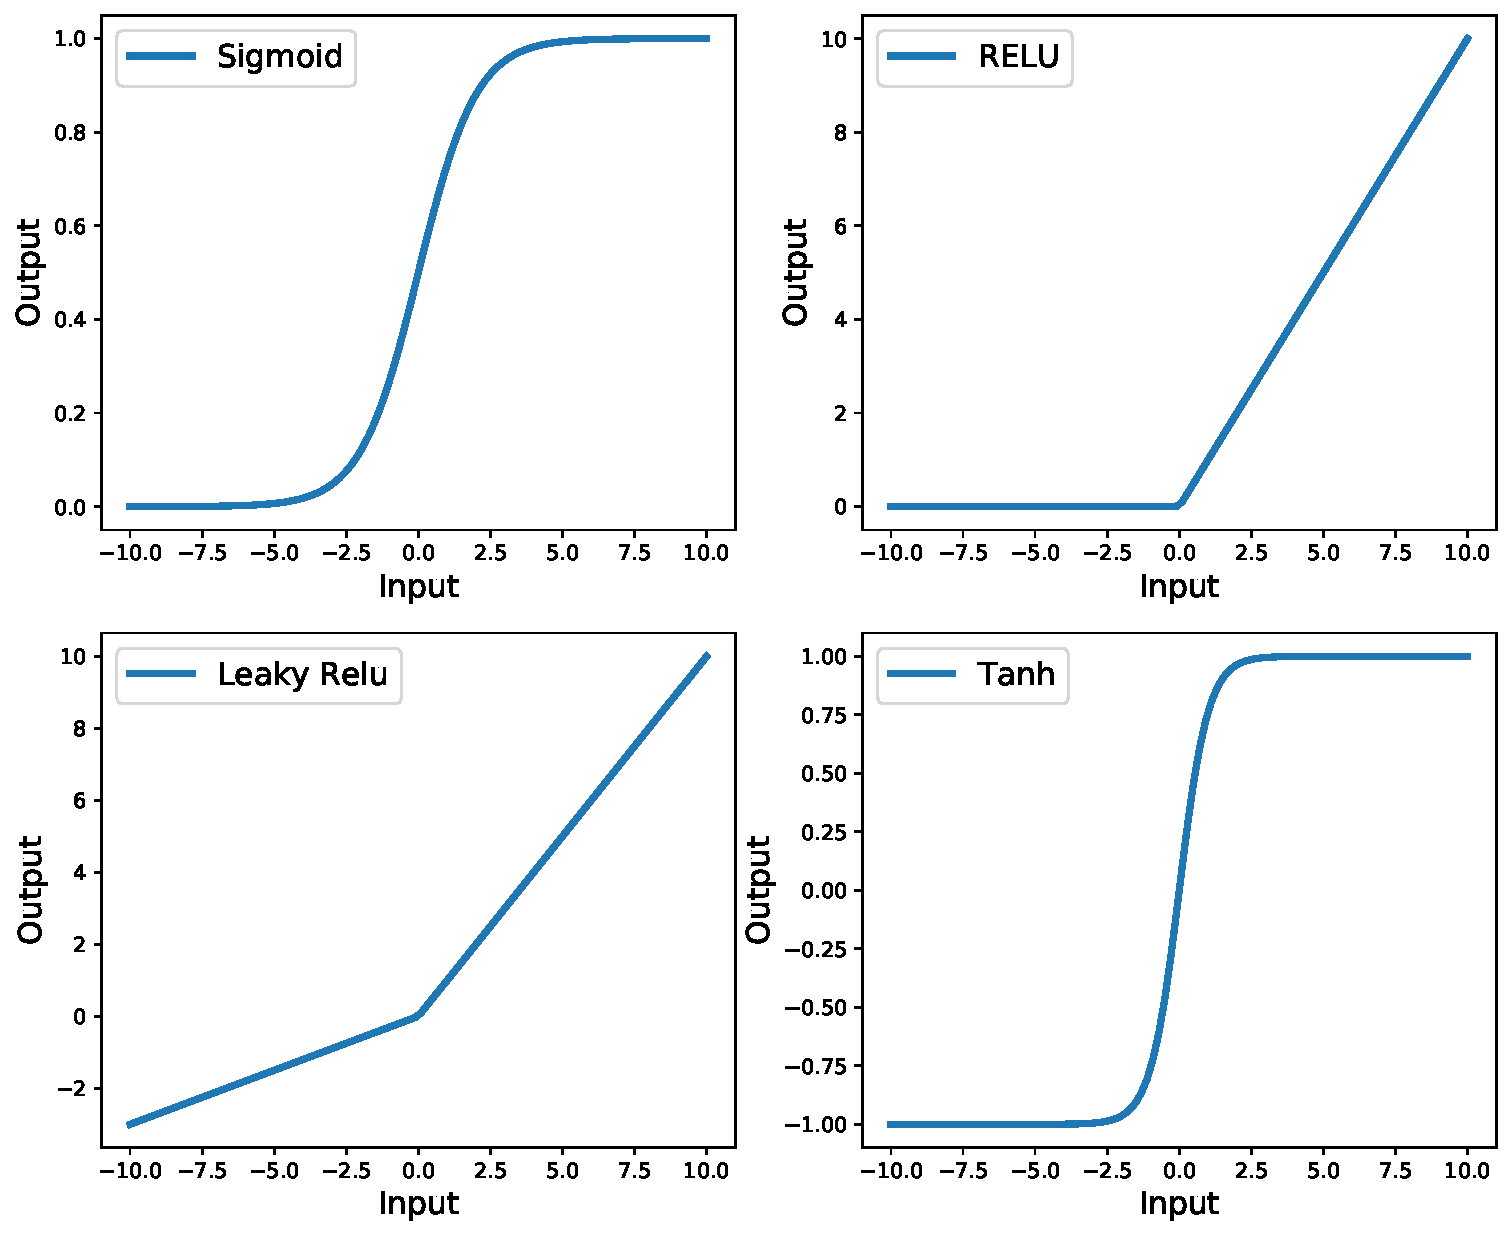
\includegraphics[width=0.8\columnwidth]{C4_cnn/activations.pdf}
	\caption[Examples of activation functions.]{There are many different activations function which are used, any function can be defined for this however, a subset of the more commonly used functions is shown here.}
	\label{machine:nn:activation:plot}
\end{figure}





%%%%%%%%%%%
%%%%%%%%%%%
\section{\label{machine:cnn}Convolutional Neural Networks}
%%%%%%%%%%%
%%%%%%%%%%%

\glspl{CNN} are a different type of deep neural network than in Sec.~\ref{machine:nn}, they are primarily used in image processing and recognition
\cite{lecun2015DeepLearning,lecun1998GradientbasedLearning,waibel1989PhonemeRecognition,krizhevsky2012ImageNetClassificationa}.
A \gls{CNN} has a similar goal to a full connected neural network; it is designed to take in data, identify different features within that data and classify what those features or combinations of those features mean.
In the context of this work the input data is a time-frequency spectrogram which may contain a simulated \gls{CW} signal.
The output is then a single number gives a probability that a signal is present.
A \gls{CNN} can learn how to identify features by being trained on many
examples of the input data which has a label.
For example, an input spectrogram with a simulated \gls{CW} signal would be labelled to have a signal.
Given the set of training examples, the many parameters of the \gls{CNN} can
be updated such that it gives the best result for any new image. 
This process is the same as neural networks in Sec.~\ref{machine:nn} and will be described in greater detail in Sec.~\ref{machine:training}.

The key features of \glspl{CNN} which distinguish them from ordinary neural networks is some additional types of layers including: Convolutional layers and max pooling layers. 


%%%%%%%%%%
%%%%%%%%%%
\subsection{Convolutional layers}
%%%%%%%%%%
%%%%%%%%%%

Convolutional layers have some similarities to fully connected layers as described in Sec.~\ref{machine:nn:structure}. 
The main difference being how the weights are applied to the inputs.
If we assume that the input to the network is some image, then a fully connected neural network would flatten this image and apply Eq.~\ref{machine:nn:neuron:equation} to the input pixels.
This involves having a separate weight for each of the input pixels in an image.
A convolutional layer however, filters the image and outputs a filtered image of the same size (the image can be a different size it depends how the layer was set up).
This convolution is defined by
\begin{equation}
\label{machine:cnn:conv:equation}
O_{i,j} = f\left( \sum_{m} \sum_{n} F_{m,n}x_{i-m,j-n}\right) ,
\end{equation}
where $O$ is the output image, $x$ is the input image, $F$ is the convolutional filter and $f$ is the activation function.
The weights of the filter $F_{m,n}$ are what are updated when the network is trained.
Figure \ref{machine:cnn:convlayer:input} shows an example of a 6x6 image and the results of filtering the image using Eq.~\ref{machine:cnn:conv:equation} with two different filters $F$. 
In this case the network has 4 parameters for each filtered image which can be updated as opposed to the 36 which a full connected network would have for a single neuron.

Figure \ref{machine:cnn:convlayer:input} demonstrates how a filter which matches a feature in an image can highlight that particular feature. 
i.e. the diagonal line in the bottom left of the input is enhanced by Filter 1, which matches that feature. 
When this type of layer is trained, the weights of the filter are updated. After training the filter weights should then ideally match the feature which is intended to be extracted from the image.

\begin{figure}[p]

    \centering
    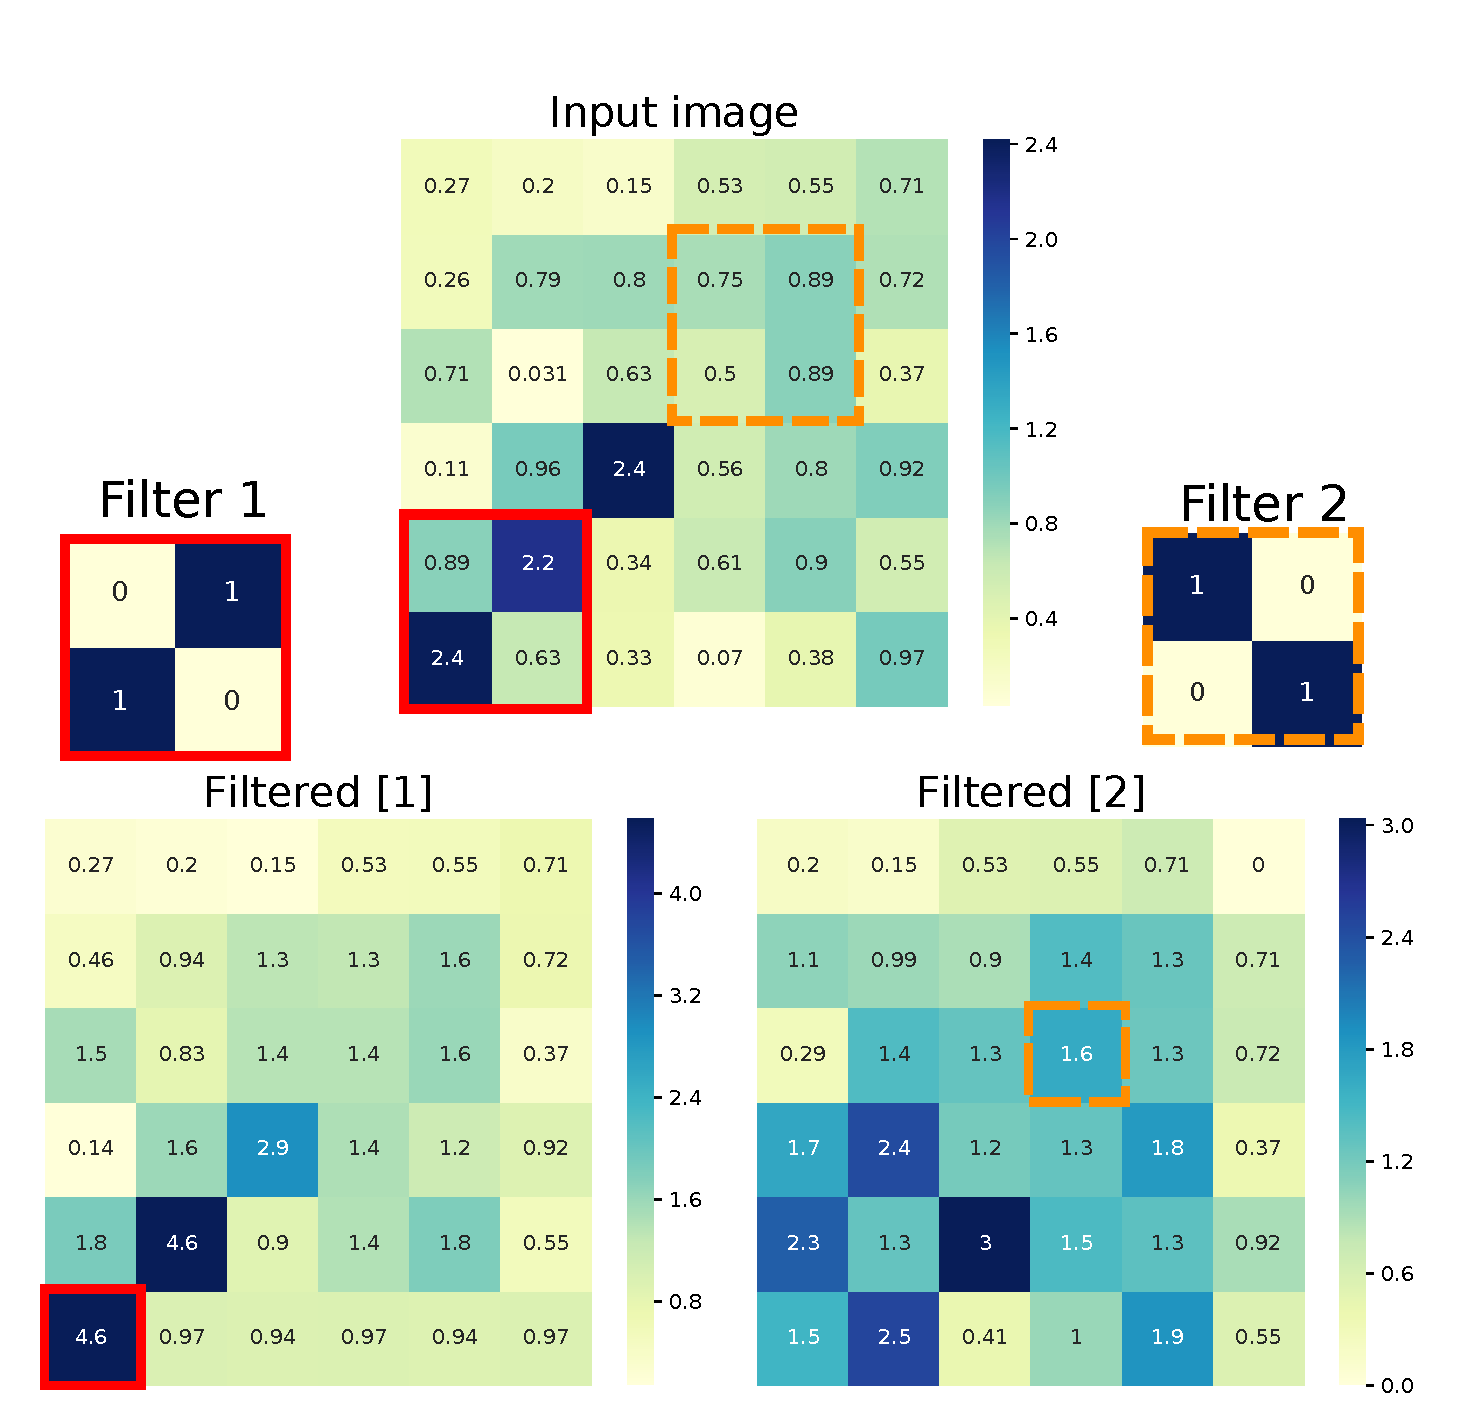
\includegraphics[width=\columnwidth]{C4_cnn/conv_filters.pdf}
    \caption[How convolutions are applied in convolutional neural networks.]{Convolutional filters can be designed to `pick out' certain features within an image. In this simple example above, the first filter (filter 1) matches the diagonal line in the bottom left of the input better than filter 2. The output filtered image the exaggerates this filter. The coefficients of the filter i.e. $F_{m,n}$ in Eq.~\ref{machine:cnn:conv:equation}, in this are set to ones and zeros.
    These are the weights which are trained by the network. In this an cases that follow, to get the same size image in the output as the input, the image is padded with zeros. I this image it was necessary to pad above and to the right of the image. The output of a convolutional layer is then the filtered images above after a bias and activation function have been applied. }
    \label{machine:cnn:convlayer:input}

\end{figure}

A convolutional layer has a number of different hyper-parameters which can be varied when setting up a \gls{CNN}.
Below I list each of the adaptable parameters and what they do.

\begin{description}
\item[Filter size] The filter size is the size and shape of the convolutional filter. In Fig.~\ref{machine:cnn:convlayer:input} we use a filter size of 2$\times$2. The filter does not have to be square, however must be less than the dimensions of the image.

\item[Number of filters] The number of filters can be any value. The convolutional layer will output the same number of filtered images as there are filters. In Fig.~\ref{machine:cnn:convlayer:input} we use two filters and therefore, the output of the layer is two images.

\item[Activation function] The activation function is generally kept the same for each of the layers, however this can be set here. The different types have been explained in Sec.~\ref{machine:nn:activation} and are applied as in Eq.~\ref{machine:cnn:conv:equation}.

\item[Stride] A normal convolutional layer applies a filter by multiplying by a filter, then shifting over by one pixel and repeating. Applying a stride mean rather than shifting by one pixel, one shifts by a number greater than one. This reduces the size of the output by the same factor of stride. i.e. if you skip one pixel (a stride of 2) then the image will be half the size on output. This has a similar affect to max-pooling which we describe in Sec.~\ref{machine:cnn:maxpool}.  
\end{description}

The convolutional layers can reduce the number of updatable parameters used in each network compared to an equivalent fully connected network.
However, the output of a convolutional layer is a number of images which are potential the same size as the input. 
This has potentially increased the size of the parameter space for the next layer.
To decrease this a type of layer known as max-pooling is used.

%%%%%%%%%
%%%%%%%%
\subsection{\label{machine:cnn:maxpool}Max pooling layers}
%%%%%%%%%%%%
%%%%%%%%%%%

Max pooling layers are designed to reduce the size of the problem whilst holding on to as much important information as possible.
These do not contain any trainable parameters.
The idea of this layer is relatively simple, it reduces the image size by taking the maximum value in a region of a given size.
Fig.~\ref{machine:cnn:maxpool:image} shows the output of the first filtered image in Fig.~\ref{machine:cnn:convlayer:input}.
The image is then reduced by a 2$\times$2 max pooling layer.
The output of max-pooling Then shows a large value in the bottom left, this is where the input image matched the filter in Fig.~\ref{machine:cnn:convlayer:input}.
This demonstrates how the max-pooling layer can hold on to important information whilst reducing the image size.

\begin{figure}[h]
    \centering
    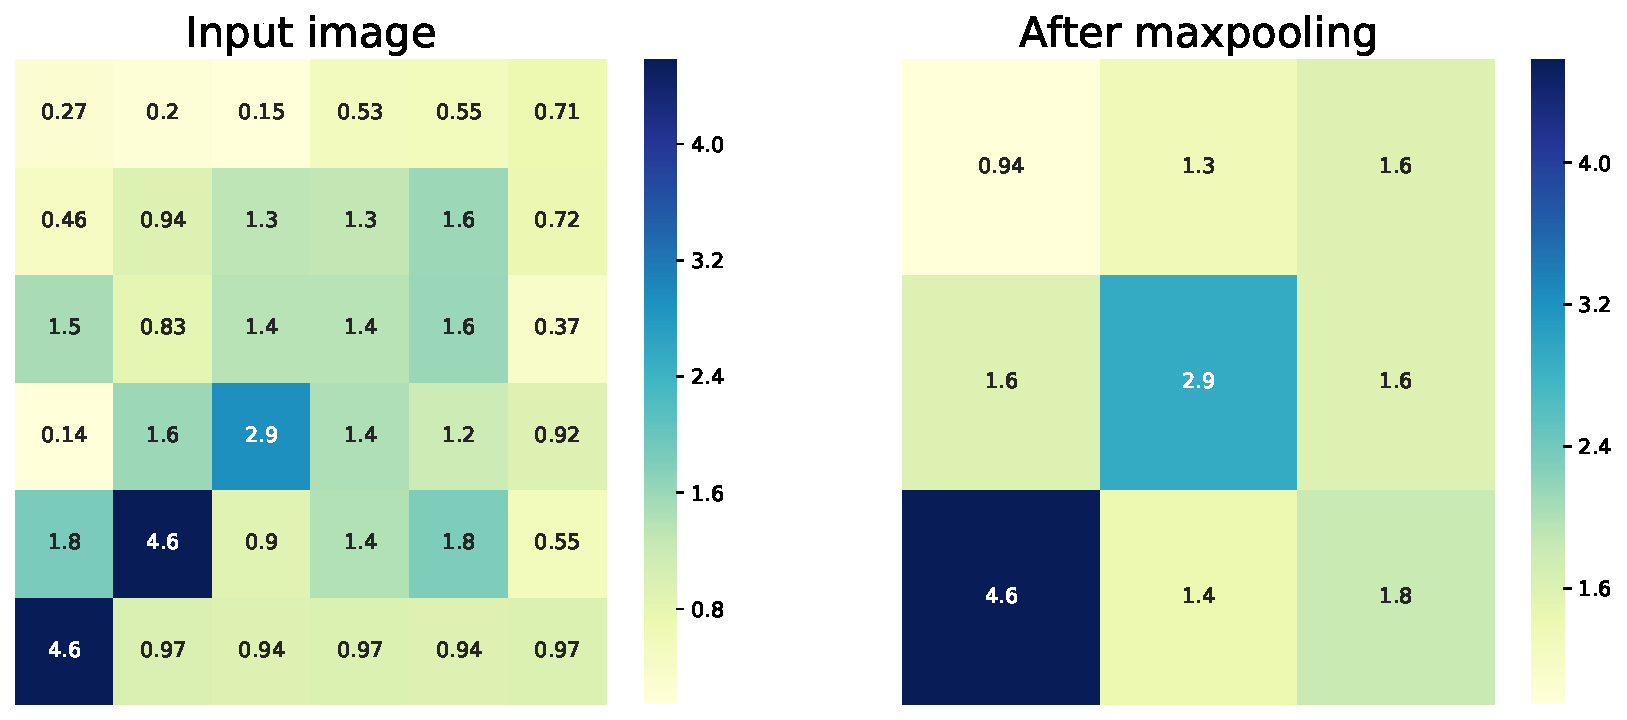
\includegraphics[width=\columnwidth]{C4_cnn/maxpool.pdf}
    \caption[How max pooling layers are applied in \glspl{CNN}.]{Max pooling layers aim to reduce the size of am image whilst retaining important information within the original image. Above shows an example where a 2$\times$2 max-pooling layer is used on the output of Filter 1 in Fig.~\ref{machine:cnn:convlayer:input}. This retains the information that the input image matches the filter in the bottom left.}n
    \label{machine:cnn:maxpool:image}
\end{figure}

%%%%%%%%%%%%%
%%%%%%%%%%%%%%
\subsection{CNN structure}
%%%%%%%%%%%%%%
%%%%%%%%%%%%%%

\glspl{CNN} are usually structured such that they can extract larger features from an input image, then the outputs from this are passed on to be classified.
The `feature extraction' part of the network consists of the convolutional layers and the max-pooling described in Sec.~\ref{machine:cnn}.
The outputs of the final max-pooling layer are then flattened and used as the input to a fully connected network.
This fully connected network the classifies these outputs into a number of classes.
Figure \ref{machine:cnn:structure:example} shows an example of the layout. 
Here an input image which is the same as in previous examples is passed onto a single convolutional layer with two different filters.
The output of two filtered images is passed to a max-pooling layer.
The two max-pooled images are flattened into 18 input neurons, this then passes through a fully connected network to a single output neuron.
This shows a simple example, however, there are many hyper-parameters of the network which can be changed.
These include: the number of filters in a convolutional layer, the number of convolutional layers and max-pooling layers, the number of hidden layers in the fully connected section and the number of neurons in the hidden layers. 
This example also shows the network being classified to a single output as this is how we use \glspl{CNN} for the following work.

\begin{sidewaysfigure}[hp]
	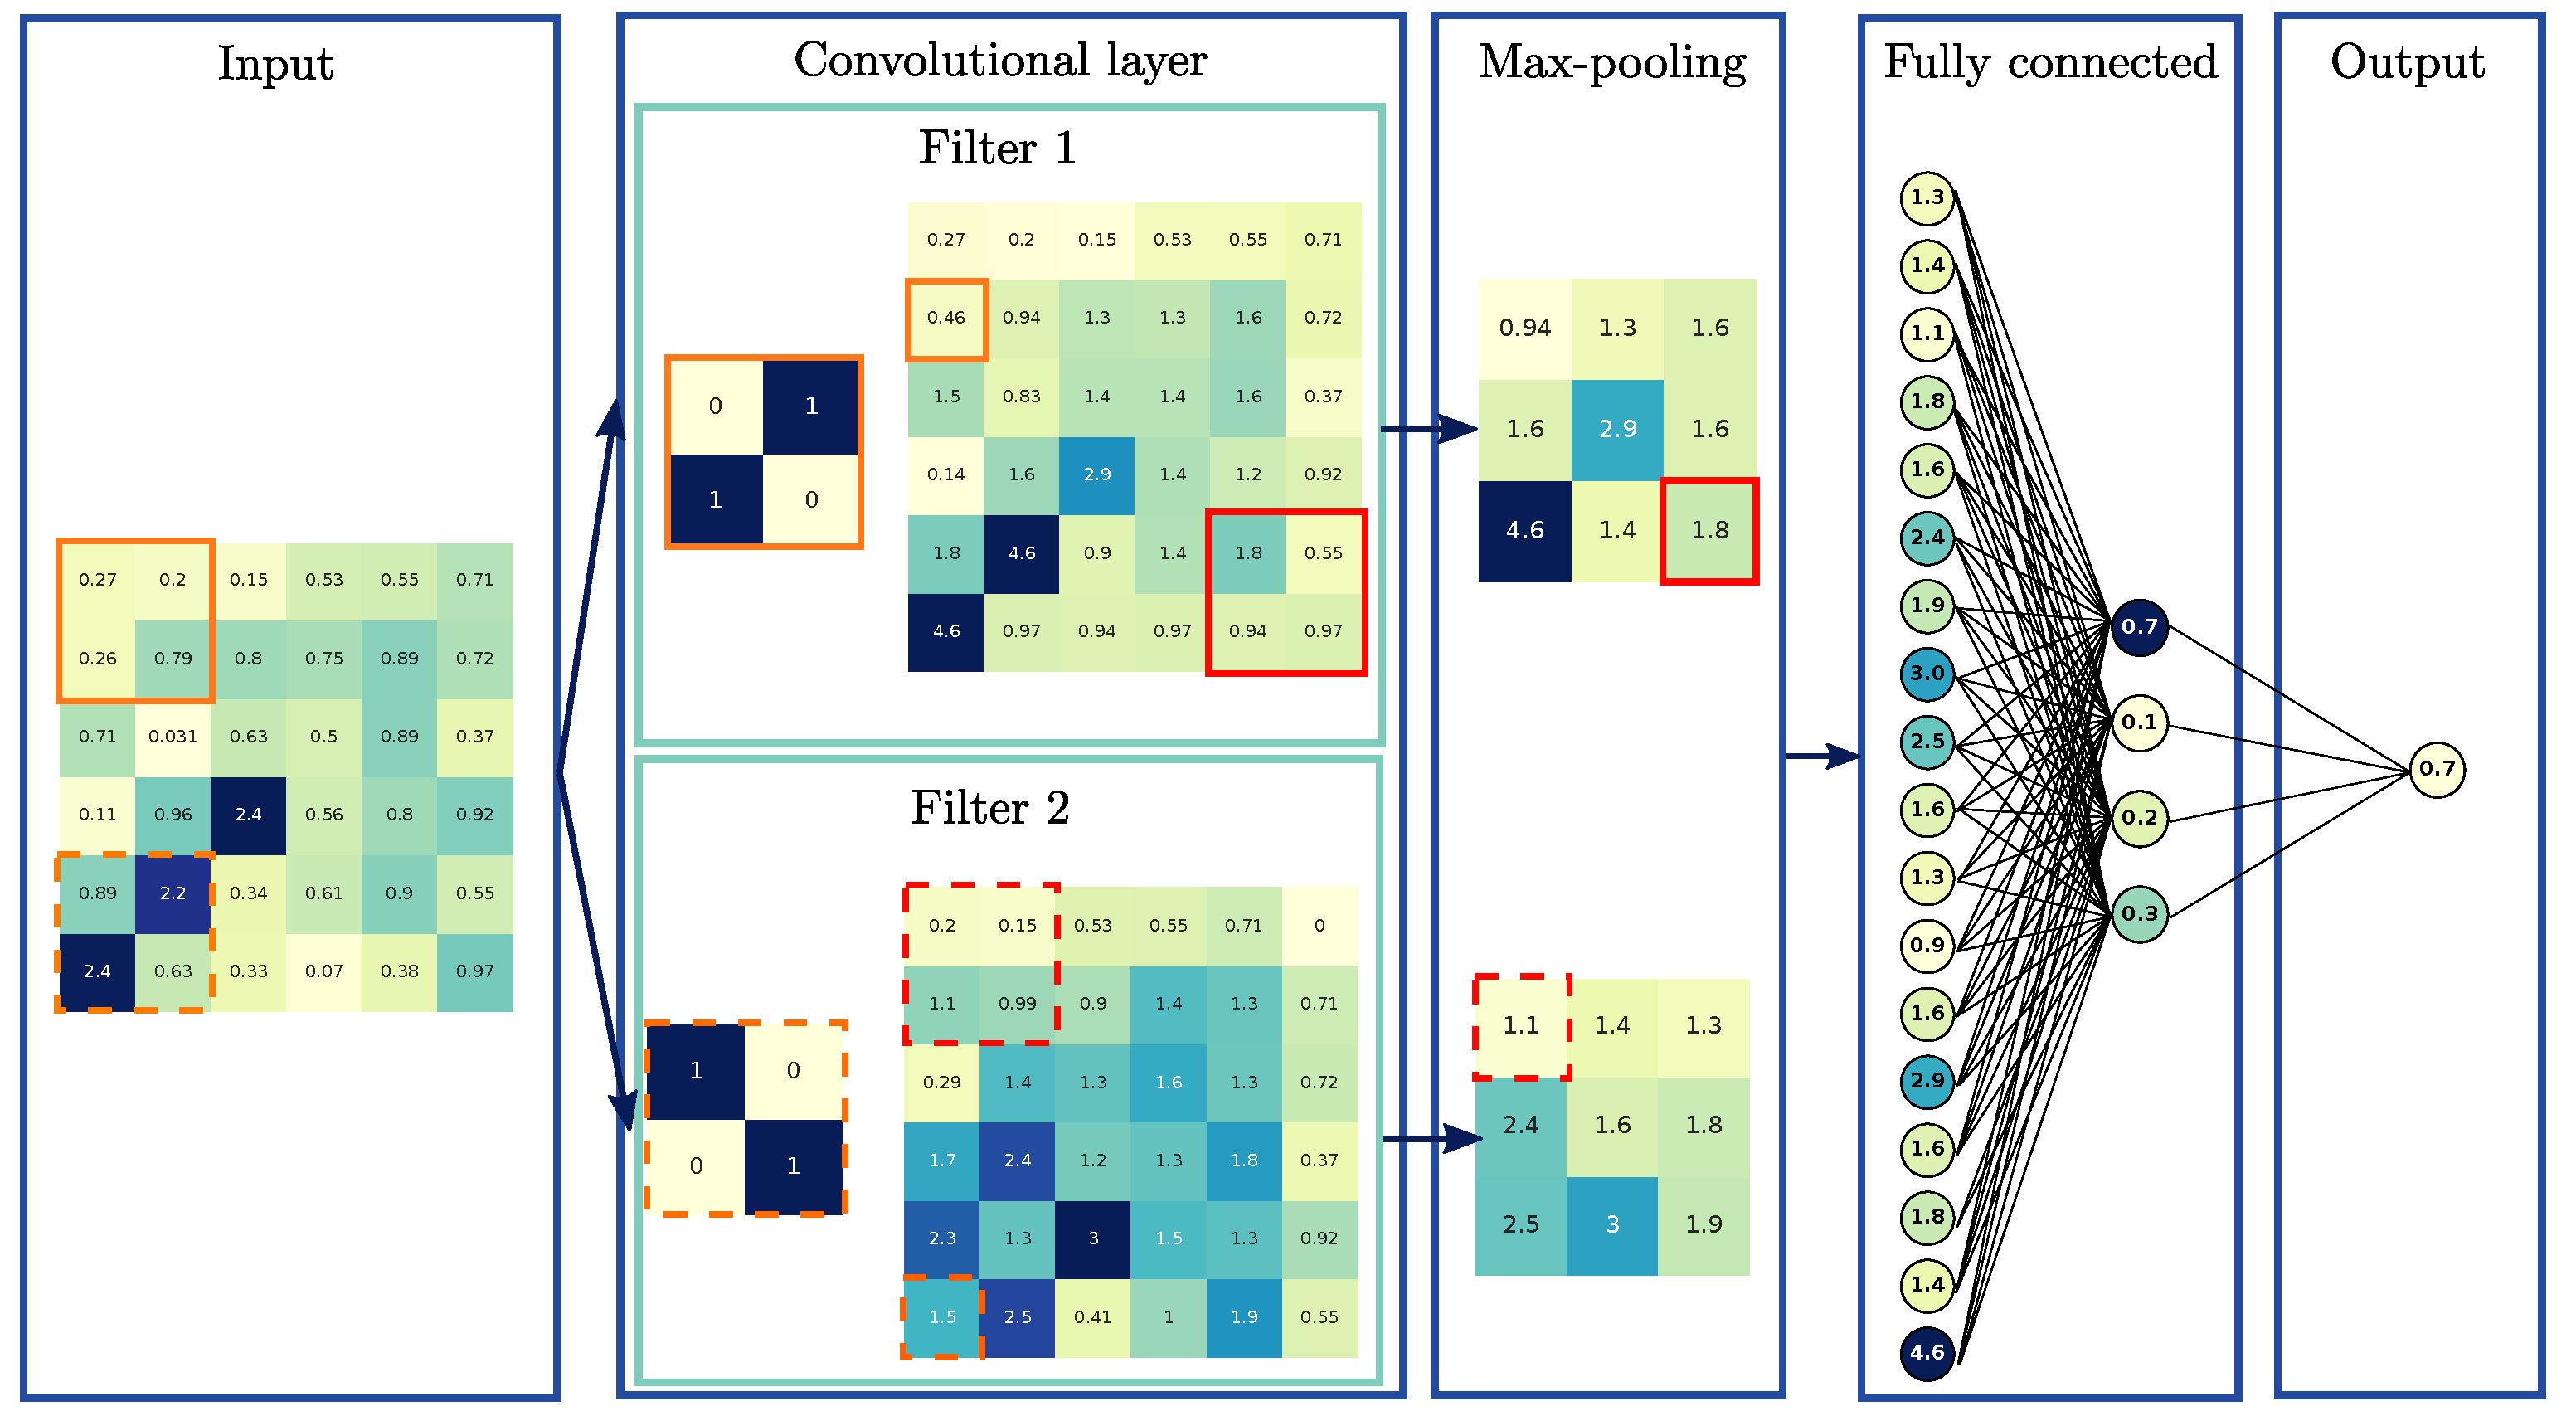
\includegraphics[width=\textwidth]{C4_cnn/cnn_structure_ex.pdf}
	\caption[Structure of \glspl{CNN}.]{Convolutional neural networks consist of two broad sections, the `feature extraction' part which is the convolutional and max-pooling layers, and the classification part which is the fully connected part of the network. This diagram shows a simple example of an image passing through a single convolutional layer with two filters, a single max-pooling layer and a simple fully connected network with a single hidden layer consisting of 4 neurons. The values in this diagram omit the use of any activation function such that the values are easier to follow. In a real network the activation functions are important.}
	\label{machine:cnn:structure:example}
\end{sidewaysfigure}


%%%%%%%%%%%%%%%%%
\section{\label{machine:training}Training}
%%%%%%%%%%%%%%%%%

% introduce training concept
%
Once the structure of the network is decided, the network needs to be trained.
This means that the weights and bias' for every neuron and filter need to be updated such
that the neural network gives a useful output. For this
work we will classify input time-frequency spectrograms into a signal or noise class using a single output neuron.
This neuron outputs a value in the range [0,1] by using a sigmoid activation function.
In our case the \gls{CNN} is trained using a process called supervised learning. 
In supervised learning, the class of each input example is know. For example, we assign a label of 1 when the
input is a time-frequency spectrogram which includes a simulated \gls{CW}
signal. Similarly a time-frequency spectrogram with no simulated signal is assigned a label of 0. 
In general when training neural networks this way, the performance of the network can be improved by increasing the number of input examples which are shown to the network.
This stops the network from over-fitting to specific examples. Instead it should generalise to the full input and learn the underlying features within the data.

\subsection{Loss function}

%Training procedure
%
Initially each of the training examples is propagated though the network to its single output value which lies between 0 and 1. Using a loss function, this output is then be compared to
the label of the input data which is either 0 or 1. There are many types of loss function which can be used, this depends on the type of problem which one wants to solve. As we are classifying
between two classes in out networks, the loss function, $L$, is the binary
crossentropy defined as
%
\begin{equation}\label{cnn:loss} 
L = -\frac{1}{N} \sum_{i}^{N} y_i\log{(p_i)} + (1-y_i)\log{(1-p_i)},
\end{equation}
%
where $p$ is the networks predicted output which has any value in the range $[0,1]$ and $y$ is the true output which has binary labels 0 or 1. This is calculated as the sum over all training examples. 
The loss function is minimised when the output matches the `truth'. This
tells the neural network how close to the truth this output is. The weights and bias' of
the neural network can be updated based on the value of this loss function. The
process of updating the weights and other parameters is called back-propagation,
and typically uses a form of gradient descent
\cite{kingma2015AdamMethod}.
Back-propagation uses the derivative of the loss function with respect to a weight to update that weight.
If changing that weight in a particular direction decreases the loss function, then the weight will be updated in that direction.
The size of the change of the weight value is related to the change in the size loss function.
This means that the weights can be updated to minimise the loss function and therefore improve the performance of the network.

%%%
%%%
\subsection{Training procedure}
%%%
%%%

The training procedure entails passing a set of training examples through the network a number of times. 
Once the entire training data set has been passed through the network (forward pass) and the weights have been updated accordingly (back propagation), the training has completed one epoch.
If the data was passed and the weights were updated a single time, the loss may decrease by is likely not at a minimum.
Passing the data through again may move the weights to a lower loss.
This process is repeated a number of times to try and find the minimum loss.
When training there the value of the loss at each epoch is monitored, the trend of the loss of the training set should always decrease. 
In general  subset of the training data is set aside and not used in the training procedure, this is known as validation data. 
After each epoch the value of the loss for this validation set can be measured, i.e. all the validation data is passed though the network. 
This can be used to monitor the training of the network. If the validation loss begins to increase then this is a sign that the network is over-fitting to the training data-set.


%%%%%%%%%%%%%%%%%%%%%%%%%%%%%%%%%%%%%%%%%%%%%%
%%%%%%%%%%%%%%%%%%%%%%%%%%%%%%%%%%%%%%%%%%%%%%%%
\section{\label{machine:cw}Application to CW search}
%%%%%%%%%%%%%%%%%%%%%%%%%%%%%%%%%%%%%%%%%%%%%%%%%
%%%%%%%%%%%%%%%%%%%%%%%%%%%%%%%%%%%%%%%%%%%%%%%

The aim for this work is to use a \gls{CNN} to classify \gls{LIGO} data into one of two classes: signal or noise.
Here the signal class refers to a \gls{CW} signal from an isolated neutron star as described in Sec.~\ref{searchcw:model}.
Noise then refers to anything else which appear in the data, from Gaussian noise to instrumental artefacts. 
In Sec.~\ref{soap:results} to reduce the effect of instrumental artefacts, each of the search sub-bands was analysed by eye to determine if a sub-band was contaminated. 
Sub-bands which contained an artefact were then removed from the search.
This is a time consuming process. The main goal of the \gls{CNN} approach is to automate this part of the search.
This section will describe how we design the network to extract features and distinguish signals from instrumental artefacts.
We will then present results form searches in a range of \gls{LIGO} observing runs which include: S6, O1 and O2.


%%%%%%%%%%%%%%%
%%%%%%%%%%%%5%%
\subsection{\label{machine:cw:structure}Network structure}
%%%%%%%%%%%%%%%
%%%%%%%%%%%%%%%

In this section the structure of the networks which are used in this analysis
are described. There are three main inputs of data for each \gls{CNN}: spectrograms, Viterbi maps and the Viterbi statistic. Each of these are different representations of the raw detector data. In this analysis we train a separate \gls{CNN} for each of
these inputs and then a further three which use these combinations of inputs:
Viterbi map + spectrogram, Viterbi map + Viterbi statistic and Viterbi map +
Viterbi statistic + spectrogram. In all of the layers excluding the output layer of each \gls{CNN}, the activation functions in Eq.~\ref{machine:cnn:conv:equation} and \ref{machine:nn:neuron:equation} are defined by a function titled `leakyRELU' \cite{maas2013RectifierNonlinearities}. 
For our output neuron a sigmoid function is
used as an activation function such that the output is limited between 0 or 1.
For a given input a \gls{CNN} can then output a value between 0 and 1. When the output value is closer to 1, the input is more likely to contain a signal. 
The output value can then be treated as a detection statistic. 
The structure of the network is shown in Fig.~\ref{machine:results:cnnlayout} and is explained below. 

\begin{description}
	\item [Viterbi statistic] This is the simplest of the networks and will
	give the exact same result as the Viterbi statistic on its own. This is a
	single neuron which takes in the Viterbi statistic applies a weight and bias
	and then passes through a sigmoid function.
	
	\item [Viterbi map] The Viterbi map \gls{CNN} takes in a down-sampled Viterbi map of size (156,89), this is described more in Sec.~\ref{machine:data:downsample}.
	This \gls{CNN} consists of two convolutional layers and 3 fully connected layers. The first layer has
	8 filters which have a size of $5\times5$ pixels, the second layer has 8
	filters with a size of $3\times3$ pixels. After each of these layers we use a
	max-pooling layer with a size of $8\times8$ pixels. This then passed into three
	fully connected layers which all have 8 neurons and used leakyRELU activation
	functions. Finally these lead to an output neuron which uses a sigmoid
	function.
	
	\item [Spectrogram] The spectrogram \gls{CNN} takes in a down-sampled spectrograms of size (156,89), this is described more in Sec.~\ref{machine:data:downsample}.
	This \gls{CNN} has an identical structure as the Viterbi map \gls{CNN}, however, takes two channels as input. The two channels are the spectrograms of two different detectors.
	
\end{description}

The next three networks are constructed from combinations of the previous described \glspl{CNN}.

\begin{description}
	\item [Viterbi map and spectrogram] To combine the spectrogram and Viterbi map network, we remove the final output neuron and its 8 weights from each of the networks. 
	The outputs from each network is then 8 neurons. These can be combined to a single sigmoid neuron which has 16 new weights.
	
	\item [Viterbi map and Viterbi statistic] In this network we combine the
	Viterbi statistic with the Viterbi map. As before, this uses the pre-trained
	Viterbi map and Viterbi statistic \glspl{CNN}. The output sigmoid neuron and corresponding weights are removed from each network. 
	The 8 neurons from the Viterbi map network and the single neuron from the Viterbi statistic network are then combined to a single neuron with 9 new weights.
	
	\item [Viterbi map, Viterbi statistic and spectrogram] This combination takes all component \glspl{CNN} from above. As before the final sigmoid output and the corresponding weights from each network are removed.
	The 8 neurons from the Viterbi map and spectrograms \glspl{CNN} and the single neuron from the Viterbi statistic are then joined into a single output neuron with 17 new weights. 
	
\end{description}

When combining \glspl{CNN} we use a process called transfer
learning~\cite{prattDiscriminabilityBasedTransfer}. This uses the pre-trained weights of the networks as a starting point to continue training. 
In our examples we found that we could fix the weights inside the pre-trained networks and just train the final 16 output weights from the neurons as in Fig.~\ref{machine:results:cnnlayout}.
These combinations of networks were chosen as the different representations of the data should contain slightly different information on the input.
For example, the Viterbi statistic contains no information on the structure of the track in the data and the Viterbi maps lost some information about lines in the band.
The addition of the spectrograms aimed to include even more information about this piece of data. 
Where when each of these are combined, the \gls{CNN} should be able to pick to important information from each of these representations.

% plot of vitmap and spectrogram structure 
%
\begin{figure}[p]
	\centering
	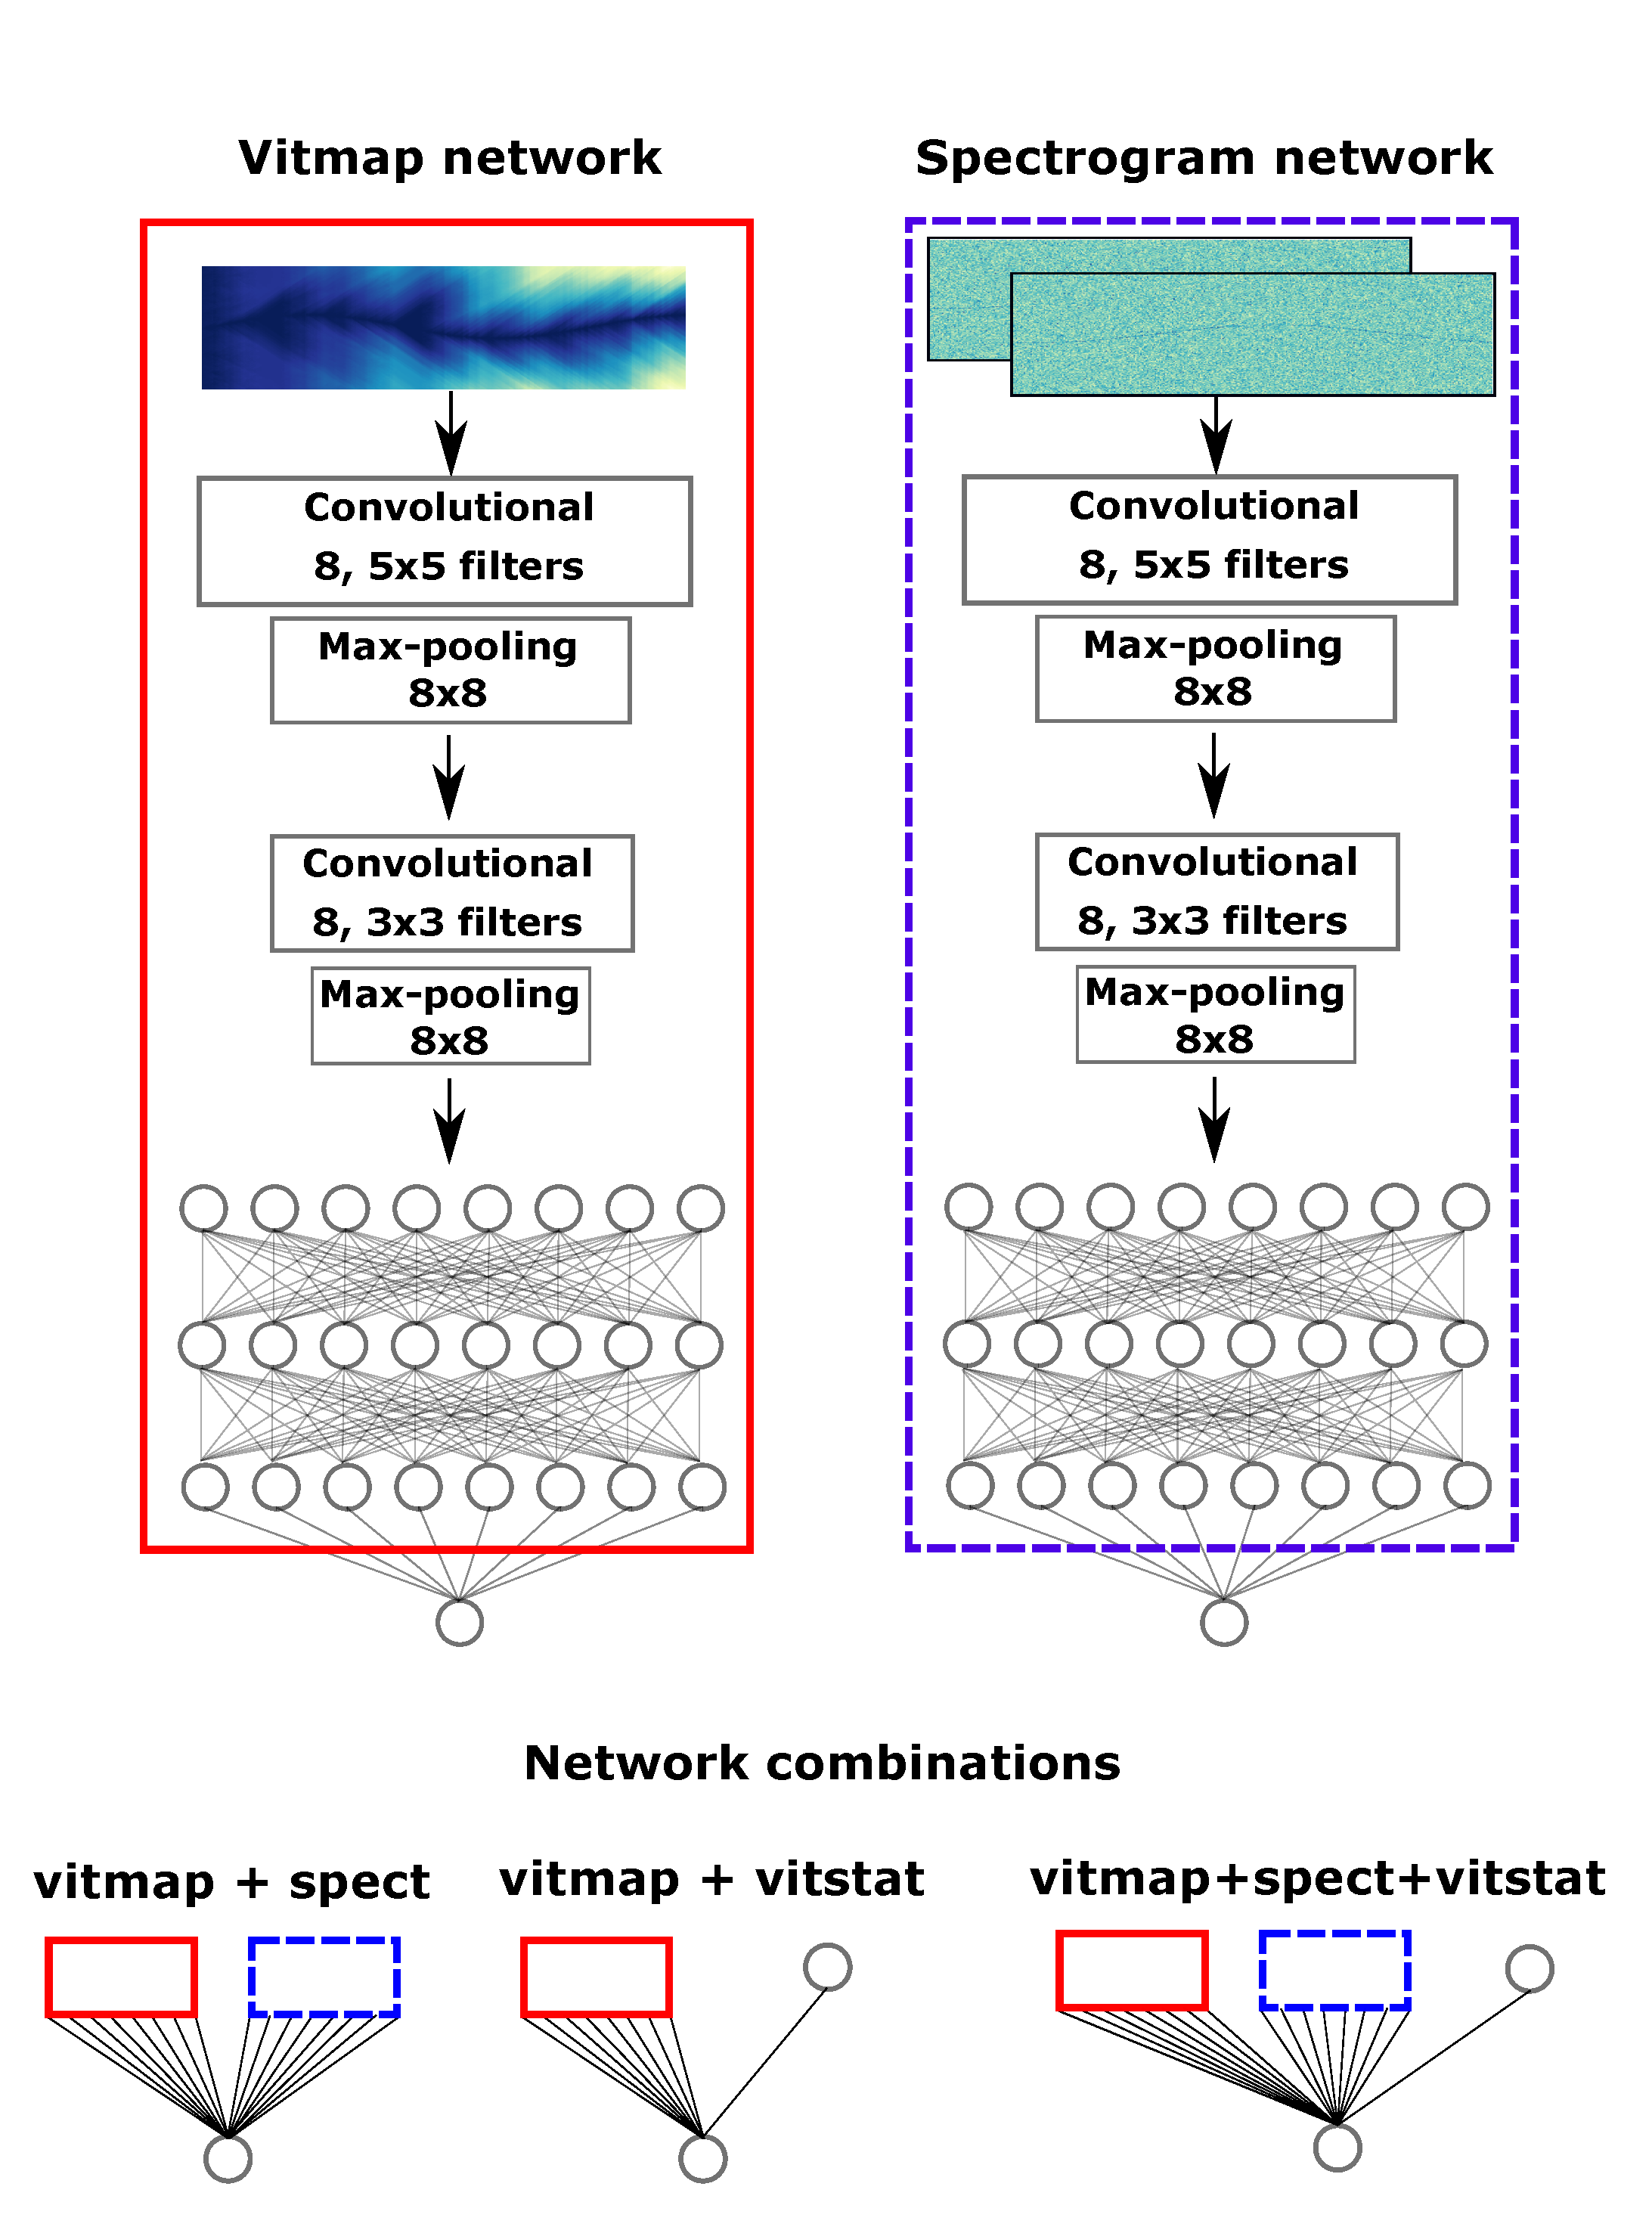
\includegraphics[width=0.9\columnwidth]{C4_cnn/networks.pdf}
	%
	\caption[Structure of \glspl{CNN} used in the search got \glspl{CW}.]{\label{machine:results:cnnlayout} The structure of the Viterbi map and
		spectrogram \glspl{CNN} used in this analysis are the same, with the difference
		that the spectrogram takes two images as input. They each use two convolutional
		layers and 3 fully connected layers before they're output to a single neuron which represents the probability of belonging to the signal class. The
		Viterbi statistic network is a single neuron that transforms the statistic into
		a number between 0 and 1 representing the probability of belonging to
		the signal class. For the combinations of networks, we remove the final
		output neuron and its 8 weights, i.e. we take the part inside the red or blue box. The 8 outputs from each network are then combined to a single neuron with 16 new weights. }
	%
\end{figure}


%%%%%%%%%%%%%%%%%%%%%%%%%%%%%%%%%%%%%%
%%%%%%%%%%%%%%%%%%%%%%%%%%%%%%%%%%%%%%
\section{\label{machine:data} Data generation}
%%%%%%%%%%%%%%%%%%%%%%%%%%%%%%%%%%%%%%
%%%%%%%%%%%%%%%%%%%%%%%%%%%%%%%%%%%%%%

% define the 3 data types that we consider
%

To train the \glspl{CNN} we need to generate many examples of data, this include the three data products above: Time-frequency spectrograms, Viterbi maps and the Viterbi statistic. 
When a \gls{CNN} is trained it needs to see examples of all possible features which could appear in the data. This include, Gaussian noise, non-Gaussian artefacts and \gls{CW} signals. 
As non-Gaussian artefacts are difficult to simulate, it is possible to use the non-Gaussian artefacts in real data as part of the training set.
Therefore, for the majority of the analysis that follows, the time-frequency spectrograms which are used to generate the Viterbi data are from real detector data. The exact observing runs used will be explained in Sec.~\ref{results}. 

For the analysis that follows there are three main sets of data: training data,
test data and search data. 
Training data uses a set of augmented (see Sec.~\ref{data:augmentation}) time-frequency spectrograms containing simulated signals and is used to train each of
the networks. 
Test data is a separate set of simulations in time-frequency spectrograms which are not augmented. These are used to generate
efficiency curves and test the network.
Search data does not contain any simulated signal injections and is used to search for real signals within the data.

% describe the idea of odd and even bands
%
When training and testing a network it is important that the networks are not
trained and tested on the same data. Otherwise the \glspl{CNN} can learn specific
features of the training data and not the underlying
distribution of features. To avoid this, the spectrograms are split into $0.1$
Hz wide sub-bands where alternating bands are designated as `odd' or `even'.
This means that bands starting with 100.1,100.3 are odd and 100.2,100.4 are
even etc. The networks can then be trained on the odd bands and tested on the
even bands and vice versa.
This then means that each time we want to search over data, we will have two final networks. One which will be run on odd bands and a separately trained network which is run on even bands. 



%%%%%%%%%%%%%%%%%%%%%%%%%%%%%%%%%%%%%%%%%%%%%%%%%%%%%%%
\subsection{\label{machine:data:injections} Signal simulations}
%%%%%%%%%%%%%%%%%%%%%%%%%%%%%%%%%%%%%%%%%%%%%%%%%%%%%%%

% describe signal injection
%
To inject the simulated signals into real data we generate a random set of signal
parameters which are drawn from prior distributions defined in
Table~\ref{data:injections:table}. The \gls{SNR} of each simulation is then uniformly distributed between 50 and 150. Where the \gls{SNR} is the integrated `recovered' \gls{SNR}. This is calculated for each time segment using the definition of optimal \gls{SNR} in \cite{prix2007SearchContinuous}, the total \gls{SNR} is then the sum of the squares of these.
The \gls{GW} amplitude $h_{0}$ is scaled based on the noise \gls{PSD} to achieve this \gls{SNR}. 
The power spectrum of the signal can then be simulated in each time segment of a time-frequency spectrogram. This is done by assuming that the spectrogram is $\chi^2$ distributed.
The the antenna pattern functions are taken into account for the given source parameters and detector such that the \gls{SNR} for each time segment is calculated.
This \gls{SNR} is spread over neighbouring frequency bins dependent on its location in frequency.
The power spectrum values can then be drawn from a non-central $\chi^2$ distribution with the non centrality parameter equal to the square of the \gls{SNR}.
Each signal is simulated in two detectors: \glspl{LIGO} H1 and L1.
The \glspl{SNR} reported below are then the sum of the squares of the \glspl{SNR} from each detector.



% Table for simulated signal priors
%
\begin{table*}
	%                                         
	\caption[Parameters used for simulations of \gls{CW} signals.]{\label{machine:data:injections:table} Table shows the upper and lower limits
		over which each signal parameter was randomized. The parameters $\alpha,\sin{\left(\delta \right)},f,\;\log{\left( \dot{f} \right)},\; \cos{\left(\iota
			\right)},\; \phi_0,\; \psi$ were sampled
		uniformly in the ranges specified in the table. The frequencies $f_{\rm l}$ and $f_{\rm u}$
		refer to the lower and upper frequency of the band that each signal is injected
		into. Excluding the distribution of frequencies $f$, all the injections parameters are sampled from the same distributions as the S6
		\gls{MDC}~\cite{walsh2016ComparisonMethods}.}
	%
	\scalebox{0.9}{
	\bgroup
	\def\arraystretch{1.5}
	\centering
	\begin{tabular}{c c c c c c c c r|}
		\hline
		\hline
		& $\alpha$ [rad]& $\sin\left(\delta \right)$ [rad] & $f$ [Hz]&
		$\log_{10}\left(\dot{f} [\rm{Hz/s}]\right)$ & $\cos{\iota}$ [rad]& $\phi$ [rad]& $\psi$ [rad]\\
		\hline
		lower bound & $0$ & $-1$ & $f_{\rm l} + 0.25$ & $-9$ & $-1$ & $0$ & $0$ \\
		\hline
		upper bound & $2\pi$ & $1$ & $f_{\rm u} - 0.25$ & $-16$ & $1$ & $2\pi$ & $\pi/2$ \\
		\hline
	\end{tabular}
	\egroup
}	
\end{table*}

%%%%%%%%%%%%%%%%%%%%%%%%%%%%%%%%%%%%%%%%%%%%%%%%%%%
\subsection{\label{machine:data:augmentation} Augmentation}
%%%%%%%%%%%%%%%%%%%%%%%%%%%%%%%%%%%%%%%%%%%%%%%%%%%

% introduce augmentation
%
To train a neural network, many examples of data from each class are needed to avoid over-fitting.
In our case when we use data between 40-500 Hz, splitting the data into 0.1 Hz wide sub-bands does not give enough data for the
networks to be trained effectively. Therefore, using a technique called data
augmentation~\cite{patrice1991TangentProp,baird1992DocumentImage} we can
artificially increase the number of training examples.
Augmentation is when data is transformed such that, to the network, it appears to be `new'
data. 
For example, by shifting a time-frequency band up and down in frequency, this appears to be a new realisation of noise which we can then inject a simulated signal into.
This would double the size of the training data-set and reduce the likelihood of over-fitting to the training data. 

% exactly what we do for augmentation
%
The augmentations are applied to the spectrograms from each of the detectors.
The augmentations that are used on each sub-band are: reversing the data in
time, flipping the data in frequency, rolling the data in time by a small
number of segments and shifting the data in frequency by a small number of
bins. As we use real data, there are gaps in time where the detectors were not
operating. We preserve the location of these gaps when augmenting the data.
When shifting the data in frequency, we shift each band up and down by 30 frequency bins (0.016 Hz) and up and down by 60 frequency bins (0.032 Hz).
When rolling the data in time, we roll each sub-band by 100 time segments (100 days). 
Fig.~\ref{machine:data:augmentation:examples} shows examples of the original data, a flip in frequency, a roll in time and a flip in time.
For each frequency shift, we flip the sub-band in time and frequency and roll the sub-band in time.
This then gives us 3 transformations for each of the 4 frequency shifts, which including the original data gives 20 times the number of training examples.

\begin{figure}
	\centering
	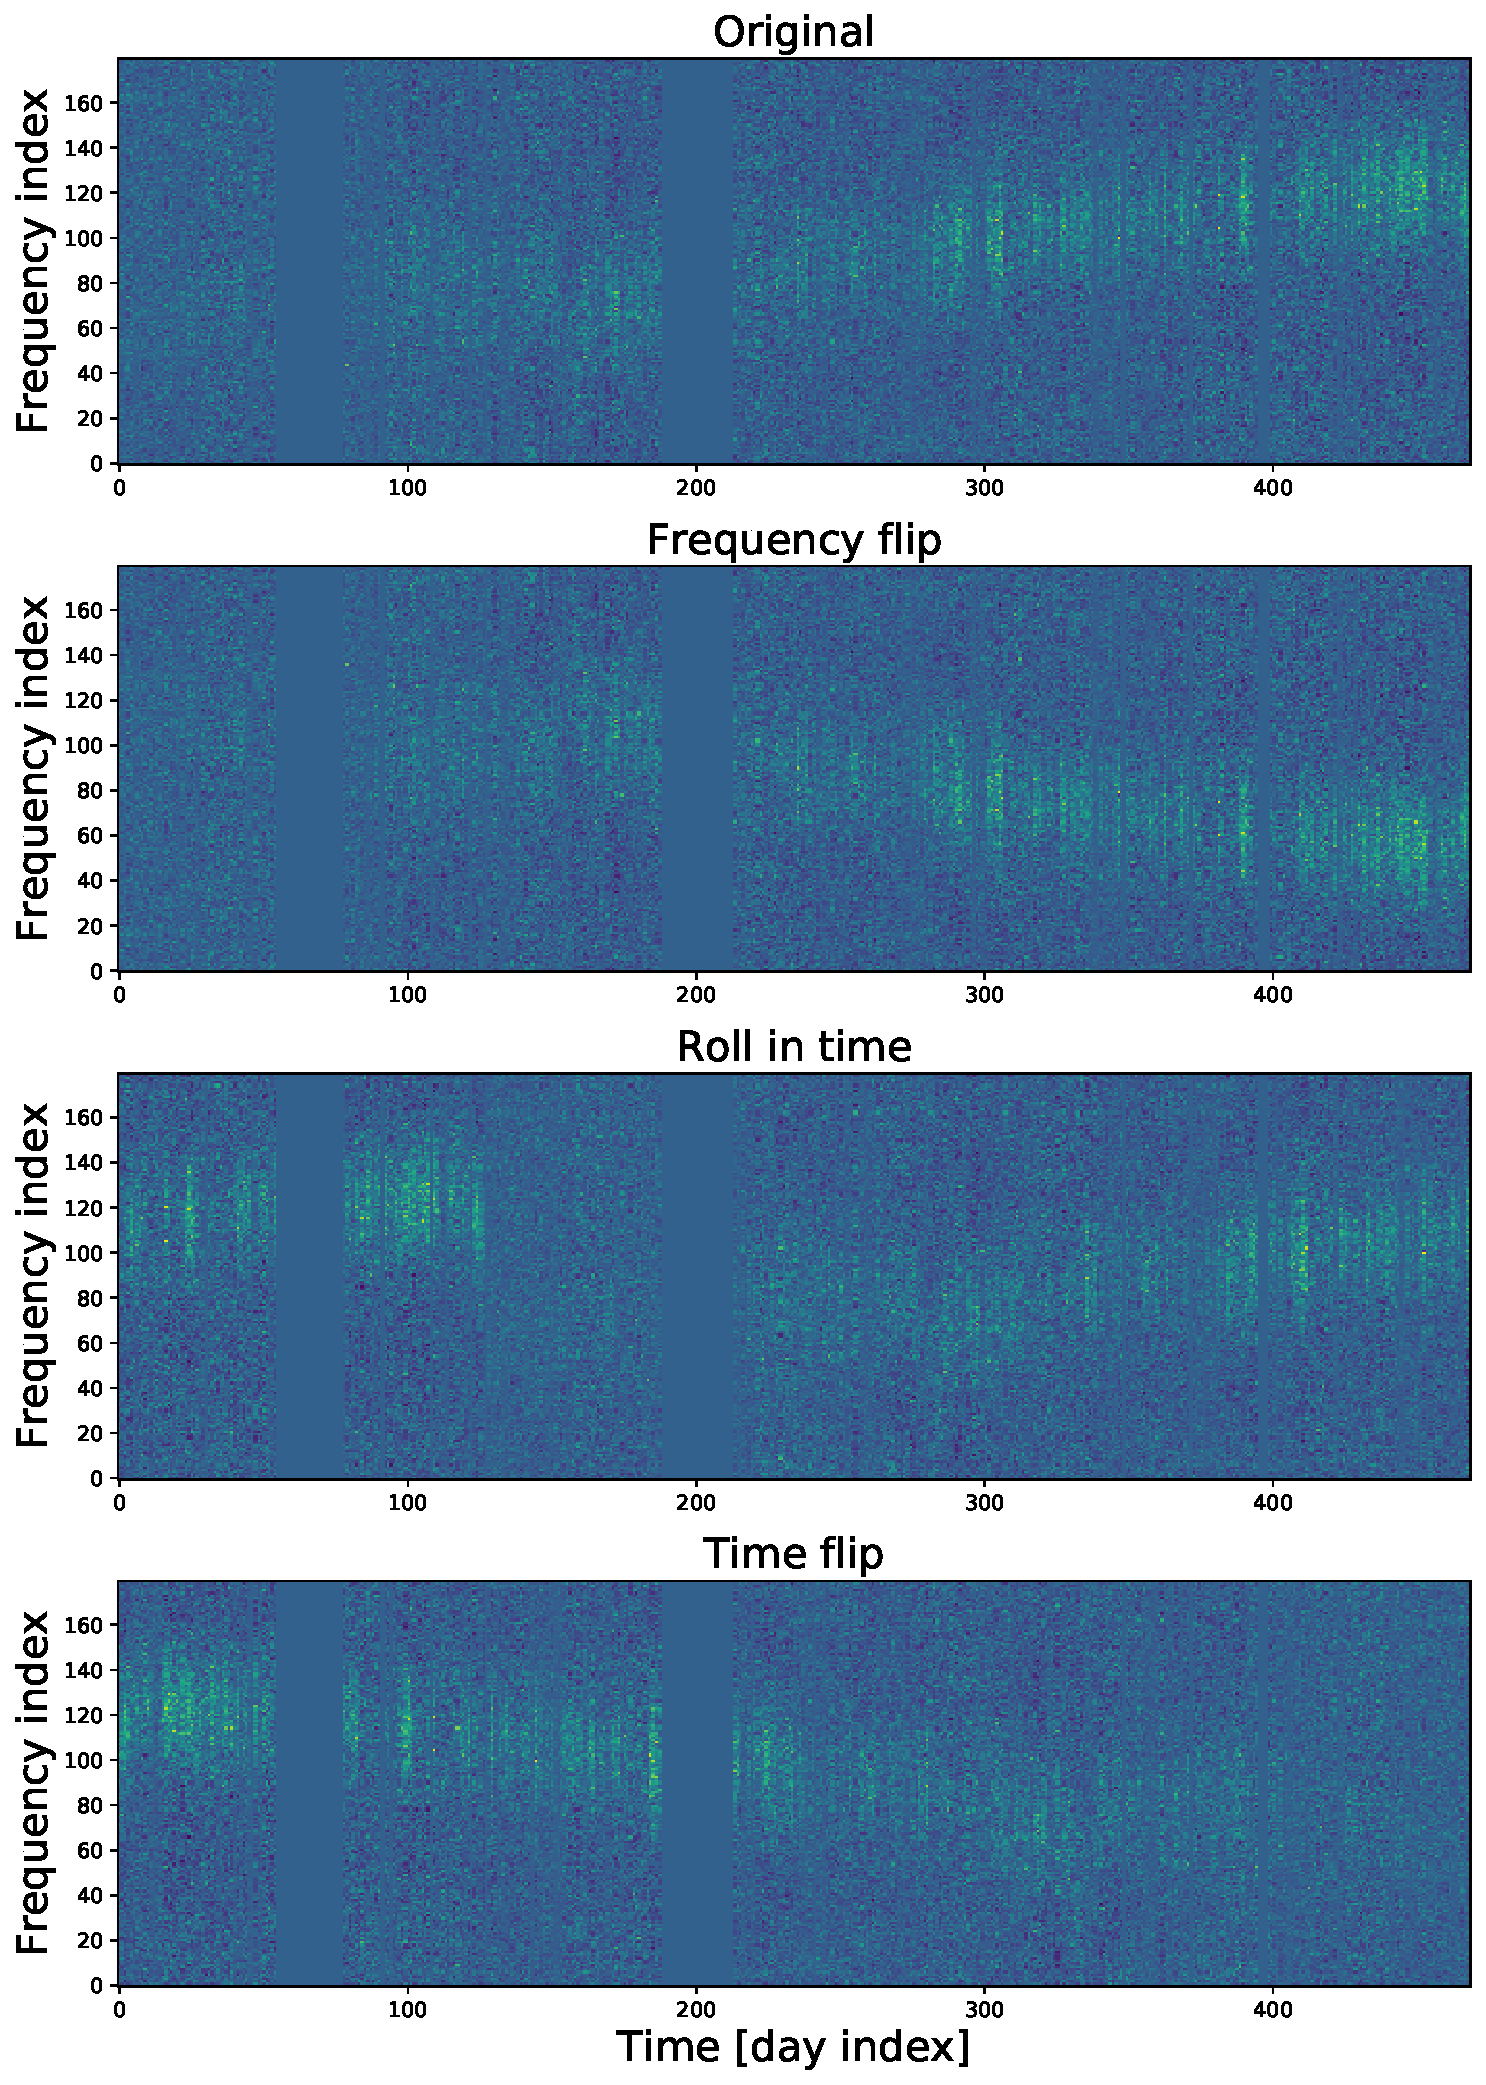
\includegraphics[width=0.8\columnwidth]{C4_cnn/augmentation.pdf}
	\caption[How data is augmented, i.e. flipping in time and frequency.]{The data is transformed by flipping the data in frequency (panel 2),
		rolling the data in time by 100 bins (panel 3) and flipping the data in time
		(panel 4). The original summed spectrogram is show in panel 1. Simulated
		signals can then be injected using this data as noise. The plots above show a
		broad wandering line to demonstrate the changes to the data when it is
		augmented, however, the majority of sub-bands contain almost Gaussian
		noise. }
	\label{machine:data:augmentation:examples}
	
\end{figure}

%%%%%%%%%%%%%%%%%%%%%%%%%%%%%%%%%%%%%%%%%%%%%%%%%
\subsection{\label{machine:data:downsample} Downsampling}
%%%%%%%%%%%%%%%%%%%%%%%%%%%%%%%%%%%%%%%%%%%%%%%%%

% introduce downsampling
%
One further issue for our data sets are their size. The spectrograms we use have a large number of pixels within them.
This means that as the spectrograms are passed through the network, there are a large number of computations.
Both this number of computations and the memory requirements of the GPU mean that training a network with a large number of data points takes longer.
We implement a few methods to reduce the size of the data: summing time segments of
spectrograms and down-sampling these summed spectrograms.  

% describe the downsampling in time and frequency
%
The spectrograms are summed over one day, i.e., every 48 time segments, as
in~\cite{bayley2019SOAPGeneralised}. This should increase the \gls{SNR} for a
given signal within a given time-frequency bin assuming that the
signal remains within the frequency bin for the majority of the time segment.
To reduce the size of the data further, the package `resize' from scikit-image
\cite{vanderwalt2014ScikitimageImage} is used, this uses interpolation to
resize the summed spectrograms to a size of (156,89) [time segments,frequency
bins]. This size was defined based on the summed spectrograms of the S6 data-set. This is 1/3 the number of summed segments in time, 1/2 the number of segments in frequency. The down-sampling is applied to the
spectrograms and vitmap. 
In \cite{bayley2019SOAPGeneralised} we demonstrated that summing spectrograms can increase the speed and sensitivity of our search.
When down-sampling the image, we found that reducing the amount of data had a small affect on the sensitivity of the \glspl{CNN} used.

%%%%%%%%%%%%%%%%%%%%%%%%%%%%%
%%%%%%%%%%%%%%%%%%%%%%%%%%%%%
\section{\label{machine:pipeline}Search pipeline}
%%%%%%%%%%%%%%%%%%%%%%%%%%%%%%%%%%%%
%%%%%%%%%%%%%%%%%%%%%%%%%%%%%%%%%

% Introduce the plan for this section
%
In previous sections each component of the search pipeline has been described,
however, described below is how each component fits together.
Figure~\ref{machine:pipeline:flow} shows a flow diagram of the pipeline. The pipeline is
run in three different ways: training the \gls{CNN}, testing the search and
running a search on real data. 

% The flow diagram showing all the parts of the process
%
\begin{figure}[htp]
	\centering
	\scalebox{0.7}{
			\centering
		

\tikzstyle{block} = [rectangle, draw, fill=blue!20, 
    text width=17em, text centered, rounded corners, minimum height=4em]
\tikzstyle{line} = [draw,line width=0.35mm, -latex']
\tikzstyle{fillnode} = [rectangle, fill=white, text centered]

\tikzstyle{blocktrain} = [rectangle, draw, fill=red!20, 
    text width=5em, text centered, rounded corners, minimum height=4em]
\tikzstyle{blocktest} = [rectangle, draw, fill=green!20, 
    text width=5em, text centered, rounded corners, minimum height=4em]
\tikzstyle{blocksearch} = [rectangle, draw, fill=black!5, 
    text width=5em, text centered, rounded corners, minimum height=4em]
\tikzstyle{blocktestbig} = [rectangle, draw, fill=green!20, 
    text width=17em, text centered, rounded corners, minimum height=4em]
\tikzstyle{blocksearchbig} = [rectangle, draw, fill=black!5, 
    text width=17em, text centered, rounded corners, minimum height=4em]
\tikzstyle{back group} = [fill=blue!20,rounded corners, draw=black!70, dashed, inner xsep=15pt, inner ysep=7pt, text centered]
\tikzstyle{back group1} = [fill=blue!20,rounded corners, draw=black!70, dashed, inner xsep=15pt, inner ysep=15pt, text centered]


\begin{tikzpicture}[node distance = 6em, auto]

    % Place node
    
  \node [block] (sft) {1.\\ SFTs from Time series};
  
  \node [block, below of=sft] (norm) {2. \\ Divide \ac{SFT} to running median and get power spectrum.};
  \node [block, below of=norm] (narrow) {3. \\ Narrowband \ac{SFT} };
  
  \node [block, below right =1.5cm and -0.9cm of narrow] (odd) {4. \\ Odd.};
  \node [block, below left =1.5cm and -0.9cm of narrow] (even) {4. \\ Even.};
  
  % odd blocks
    
  \node [blocktest,below of= odd] (testodd) {5b.\\ Test data};
  \node [blocktest, below of= testodd] (testsumodd) {6b. \\Test data};
  \node [blocktest, below of=testsumodd] (testlookupodd) {7b. \\ Test data};
  \node [blocktest, below of=testlookupodd] (testdownsampodd) {8b. \\  Test data};
  \node [below of= testdownsampodd](testblankodd) {};
    
  \node [blocktrain, left of= testodd] (trainodd) {5a.\\ Training data};
  \node [blocktrain, below of= trainodd] (trainsumodd) {6a. \\Training data};
  \node [blocktrain, below of=trainsumodd] (trainlookupodd) {7a. \\ Training data};
  \node [blocktrain, below of=trainlookupodd] (traindownsampodd) {8a. \\  Training data};
  \node [blocktrain, below of=traindownsampodd] (trainnetworkodd) {9. \\ Train `odd' \ \ac{CNN}};

  \node [blocksearch,right of=testodd] (searchodd) {5c.\\ Search data};
  \node [blocksearch, below of= searchodd] (searchsumodd) {6c. \\Search data};
  \node [blocksearch, below of=searchsumodd] (searchlookupodd) {7c. \\ Search data};
  \node [blocksearch, below of=searchlookupodd] (searchdownsampodd) {8c. \\  Search data};
  \node [below of= searchdownsampodd](searchblankodd) {};
  
  \node [blocktest, below = 1.4cm of testblankodd] (testclassifyodd) {10b.\\ Test data};
  \node [blocksearch, below = 1.4cm of searchblankodd] (searchclassifyodd) {10c.\\ Search data};

   
  % even blocks]
  
    \node [blocksearch,below of=even] (searcheven) {5c.\\ Search data};
  \node [blocksearch, below of= searcheven] (searchsumeven) {6c. \\Search data};
  \node [blocksearch, below of=searchsumeven] (searchlookupeven) {7c. \\ Search data};
  \node [blocksearch, below of=searchlookupeven] (searchdownsampeven) {8c. \\ Search data};
  \node [below of= searchdownsampeven](searchblankeven) {};
  
  \node [blocktest,left of= searcheven] (testeven) {5b.\\Test data};
  \node [blocktest, below of= testeven] (testsumeven) {6b. \\Test data};
  \node [blocktest, below of= testsumeven] (testlookupeven) {7b. \\Test data};
  \node [blocktest, below of=testlookupeven] (testdownsampeven) {8b. \\ Test data};
  \node [below of= testdownsampeven](testblankeven) {};
  
  \node [blocktrain, right of= searcheven] (traineven) {5a.\\ Training data};
  \node [blocktrain, below of= traineven] (trainsumeven) {6a. Training data};
  \node [blocktrain, below of=trainsumeven] (trainlookupeven) {7a. \\Training data};
  \node [blocktrain, below of=trainlookupeven] (traindownsampeven) {8a. \\ Training data};
  \node [blocktrain, below of=traindownsampeven] (trainnetworkeven) {9. \\ Train `even'  \ \ac{CNN}};

  
  \node [blocktest, below = 1.4cm of testblankeven] (testclassifyeven) {10b.\\ Test data};
  \node [blocksearch, below = 1.4cm of searchblankeven] (searchclassifyeven) {10c.\\ Search data};
  
% background blocks  
  
\begin{scope}[on background layer]
   
    \node (bkgen) [back group] [fit=(trainodd) (testodd) (searchodd) (traineven) (testeven) (searcheven) ] {5.\\Injections};
    
    \node (bksum) [back group] [fit=(trainsumodd) (testsumodd) (searchsumodd) (trainsumeven) (testsumeven) (searchsumeven)] {6.\\Sum spectrograms over \\1 day};
    
    \node (bksoap) [back group] [fit=(trainlookupodd) (testlookupodd) (searchlookupodd) (trainlookupeven) (testlookupeven) (searchlookupeven)] {7.\\Generate lookup tables \\and\\ run SOAP search.};
    
    \node (bkdown) [back group] [fit=(traindownsampodd) (testdownsampodd) (searchdownsampodd) (traindownsampeven) (testdownsampeven) (searchdownsampeven)] {8.\\Downsample spectrograms\\ and vitmaps.};
    
    \node (bkclassodd) [back group1] [fit=(testclassifyodd) (searchclassifyodd)] {};
     
    \node (bkclasseven) [back group1] [fit=(testclassifyeven) (searchclassifyeven)] {};

    
 \end{scope}
 
   % search and testing
  
  \node [blocktestbig, below right =1.1cm and -3.5cm of bkclasseven] (output) {11c.\\ Generate efficiency curves from test data.};
  \node [blocksearchbig, below left= 1.1cm and -3.5cm of bkclassodd] (outputsearch) {11a.\\ Take top 1\% of search bands for followup.};
  
  % Draw edges
  \path [line] (sft) -- (norm);
  \path [line] (norm) -- (narrow);
  
  % even lines
  
   \path [line] (narrow) -- (even);
  
  \path [line] (even) -- (testeven);
  \path [line] (even) -- (traineven);
  \path [line] (even) -- (searcheven);
  
  \path [line,red!60] (traineven) -- (trainsumeven.north);
  \path [line,green!60] (testeven.south) -- (testeven.south|-testsumeven.north);
  \path [line,black!60] (searcheven.south) -- (searcheven.south|-searchsumeven.north);
  
  \path [line,green!60] (testeven.south|-testsumeven.south) -- (testeven.south|-testlookupeven.north);
  \path [line,red!60] (traineven.south|-trainsumeven.south) -- (traineven.south|-trainlookupeven.north);
  \path [line,black!60] (searcheven.south|-searchsumeven.south) -- (searcheven.south|-searchlookupeven.north);
  
  \path [line,green!60] (testeven.south|-testlookupeven.south) -- (testeven.south|-testdownsampeven.north);
  \path [line,red!60] (traineven.south|-trainlookupeven.south) -- (traineven.south|-traindownsampeven.north);
  \path [line,black!60] (searcheven.south|-searchlookupeven.south) -- (searcheven.south|-searchdownsampeven.north);
  
  \path [line,red!60] (traindownsampeven) -- (trainnetworkeven);
  \path [line,green!60] (testdownsampeven) -- (testclassifyeven);
  \path [line,black!60] (searchdownsampeven) -- (searchclassifyeven);
  
  %\path [line,black!60] (searcheven.south|-searchdownsampeven.south) -- (searcheven.south|-classifyeven.north);
  %\path [line,green!60] (testeven.south|-testdownsampeven.south) -- (testeven.south|-classifyeven.north);
  
  \path [line,red!60] (trainnetworkeven) -- (bkclassodd);
  
  %% odd lines
  
   \path [line] (narrow) -- (odd);
  
  \path [line] (odd) -- (testodd);
  \path [line] (odd) -- (trainodd);
  \path [line] (odd) -- (searchodd);
  
  \path [line,red!60] (trainodd) -- (trainsumodd.north);
  \path [line,green!60] (testodd.south) -- (testodd.south|-testsumodd.north);
  \path [line,black!60] (searchodd.south) -- (searchodd.south|-searchsumodd.north);
  
  \path [line,green!60] (testodd.south|-testsumodd.south) -- (testodd.south|-testlookupodd.north);
  \path [line,red!60] (trainodd.south|-trainsumodd.south) -- (trainodd.south|-trainlookupodd.north);
  \path [line,black!60] (searchodd.south|-searchsumodd.south) -- (searchodd.south|-searchlookupodd.north);
  
  \path [line,green!60] (testodd.south|-testlookupodd.south) -- (testodd.south|-testdownsampodd.north);
  \path [line,red!60] (trainodd.south|-trainlookupodd.south) -- (trainodd.south|-traindownsampodd.north);
  \path [line,black!60] (searchodd.south|-searchlookupodd.south) -- (searchodd.south|-searchdownsampodd.north);
  
  \path [line,red!60] (traindownsampodd) -- (trainnetworkodd);
  \path [line,green!60] (testdownsampodd) -- (testclassifyodd);
  \path [line,black!60] (searchdownsampodd) -- (searchclassifyodd);
  
  %\path [line,black!60] (searchodd.south|-searchdownsampodd.south) -- (searchodd.south|-classifyodd.north);
  \%path [line,green!60] (testodd.south|-downsampodd.south) -- (testodd.south|-classifyodd.north);
  
  \path [line,red!60] (trainnetworkodd) -- (bkclasseven);
  
  % search and test
  
  \path [line,green!60] (testclassifyeven) -- (output);
  \path [line,black!60] (searchclassifyeven) -- (outputsearch);
  
  \path [line,green!60] (testclassifyodd) -- (output);
  \path [line,black!60] (searchclassifyodd) -- (outputsearch);
  
  % final labels over lines
  
   \node[fillnode,below] at (bkclasseven.south) {Classify sub-bands with \ `odd' \ac{CNN}};
   
   \node[fillnode,below] at (bkclassodd.south) {Classify sub-bands with \ `even' \ac{CNN}};
 
    
\end{tikzpicture}}
	\caption[Flow diagram for entire SOAP and \gls{CNN} search.]{\label{machine:pipeline:flow} This diagram shows the SOAP pipeline from start to finish. There are three main sections: Training (red), Testing (green) and Searching (grey) for both the odd and even bands. The blue sections mean that the same operations is done in all cases.}
	
\end{figure}

% describe the elements of the flow diagram
%
\begin{description}
	%    
	\item[1. SFTs] Generate 1800s long \glspl{SFT} from detector time-series
	data. \glspl{SFT} of this length are a standard set for \gls{CW} searches which are continuously generated during observing runs by members of the \gls{LIGO} collaboration. 
	%   
	\item[2. Normalising] The \glspl{SFT} are then divided by their running median with a window width of 100 frequency bins.
	If we assume the resulting \glspl{SFT} to be $\chi^2$ distributed, we can apply a correction factor using LALSuite code {\tt XLALSFTtoRngmed} \cite{ligoscientificcollaboration2018LIGOAlgorithm} such that their power spectrum has a mean of $\sim 1$. 
	By then multiplying this by 2, the noise like parts of the spectrum are $\chi^2$ distribution with two degrees of freedom.
	
	%
	\item[3. Narrowbanding] The computational efficiency can be improved if the data is split into narrow bands.
	This is because the analysis can be completed on each band in parallel on separate CPU nodes. 
	In this search the spectrograms are split into $2.1$ Hz wide bands every $2$ Hz, i.e.
	100.0-102.1, 102.0-104.1 etc. The bands are $2.1$ Hz wide as the analysis on each node will further split the data into 0.1 Hz wide sub-bands. 
	The overlap then allows the sub-band from 1.95-2.05 to be calculated on a node.
	This band size was chosen based on the available
	computational memory at the time. 
	%    
	\item[4. Band splitting] A \gls{CNN} should not be trained on the same
	data that it will be tested on.
	For this reason, each of the $0.1$ Hz wide sub-bands are split
	into `odd' or `even' bands. A \gls{CNN} can then be trained on even bands and tested on odd bands and vice versa.
	%
	\item[5a. Training data generation] To generate training data the process is
	the same as described in Sec.~\ref{machine:data}. Each of the $0.1$ Hz sub-bands is
	`augmented' as in Sec.~\ref{machine:data:augmentation}. For each of the augmented
	bands, the data is duplicated such that there is a second copy of every augmented band. 
	In the copied set of bands, signals are injected into them with
	\glspl{SNR} in the range 50-150. This gives us and example for a noise class and
	a signal class. There are two of these sets, one for `even' bands and
	one for `odd'.
	%
	\item[5b. Test data generation] For test data, signals following the parameters in
	Tab.~\ref{machine:data:injections:table} are injected in to 50\% of the $0.1$ Hz
	sub-bands. These signal have and \gls{SNR} in the range 20-200. The \gls{SNR} range here is wider than the training set as a method to test how the trained networks perform s on a wider range od \glspl{SNR}. Here we again have a
	set for `odd' and a set for `even'.
	%    
	\item[5c. Search data] This data is generated such that we can search for a
	real signal. The sub-bands described in part 4 are now overlapping by 0.05 Hz.
	This means that if there is an astrophysical signal it should be fully contained within at
	least one sub-band. We do assume that a signals frequency does not drift by more than 0.1 Hz, which is assumed to be true for isolated neutrons stars $< 500$ Hz.  There are both `odd' and `even' versions of this search data.
	%
	\item[6. Summing spectrogram] As in~\cite{bayley2019SOAPGeneralised} the
	spectrograms are summed over one day, i.e., every 48 time segments (1 day) of
	the spectrogram are summed. This is done separately for each of the 6 data-sets
	(3 for `odd', 3 for `even'). 
	%     
	\item[7. Generate lookup tables and run SOAP search] Before the SOAP search is
	run, the line-aware statistic lookup tables need to be generated as
	in~\cite{bayley2019SOAPGeneralised}. Then for each of the 6 data-sets (3 for
	`odd', 3 for `even') the SOAP search is run separately. 
	%     
	\item[8. Down-sample data] At this stage there are four elements which are
	saved for each of the 6 data-sets. The two spectrograms, the Viterbi maps and
	the Viterbi statistic. The spectrograms and the Viterbi maps are down-sampled
	to a size of ($156\times 89$) using interpolation from scikit-image's
	resize~\cite{vanderwalt2014ScikitimageImage}. This size was chosen based on the
	S6 \gls{MDC} data-set, where this is 1/3 the length in time and 1/2 the width in
	frequency of the summed spectrograms. 
	This was chosen such that the \glspl{CNN} trained efficiently and still achieved a reasonable sensitivity. 
	%
	\item[9. Train Networks] The down-sampled training data is then used to train a
	\glspl{CNN}. One \gls{CNN} is trained on `odd' bands and a different \gls{CNN} with
	the same structure is trained on `even' bands. 
	%
	\item[10b. Run search on test data] The trained \glspl{CNN} from part 9 are then
	used to classify each sub-band in the test data with injections, this returns a
	statistic on the range $[0,1]$. The close the value is to 1 the more likely it is from an astrophysical signal, therefore,  the statistic can be interpreted as an estimate of the probability of a signal being present. Here the \gls{CNN}
	trained on the `odd' bands is tested using the `even' bands and vice
	versa. The algorithms are run on this test data to asses the sensitivity of the analysis.
	%
	\item[10c. Run search on real data] The trained \glspl{CNN} from part 9 are then
	used to classify each sub-band in the search data, this returns a statistic in
	$[0,1]$. This statistic is the same as in part 10b. 
	Once again the \gls{CNN} trained on the `odd' bands is tested using
	the `even' bands and vice versa.
	%        
	\item[11a. Signal candidates] The signals which have a statistic in the top
	1\% can be taken as potential candidates. 
	This can then potentially be followed up with other \gls{CW} search methods. 
	%    
	\item[11c. Efficiency curves] The output statistics from the test data-set (11b.) can
	be plotted against \gls{SNR} to see how the network classified signals with the
	\gls{SNR} of the injection. This can potentially be extended to other signal parameters also. 
	Then the efficiency curves can be generated, this is described in further detail in Sec.~\ref{machine:results:sensitivity}.
	
	
\end{description}





%%%%%%%%%%%%%%%%%%%%%%%%%%%%
%%%%%%%%%%%%%%%%%%%%%%%%%%%%
\section{\label{machine:results}Results}
%%%%%%%%%%%%%%%%%%%%%%%%%%%%
%%%%%%%%%%%%%%%%%%%%%%%%%%%%

% a general introduction statement about the results
%
The networks described in Sec.~\ref{machine:cw:structure} were trained and tested on
four different data-sets: the S6 \gls{MDC} as
in~\citep{bayley2019SOAPGeneralised,walsh2016ComparisonMethods}, our own
injections into O2 data, Gaussian noise which had the same gaps and noise
floor as the S6 data-set, and our own injections into real S6 data. Each of
the searches use training and testing data in the frequency range of 100-400 Hz,
except the S6 \gls{MDC} which uses data in the range 40-500 Hz for testing and
training. 

%%%%%%%%%%%%%%%%%%%%%%%%%%%%%%%%%%%%%%%%%%%%%%%%%%%%%%%%
\subsection{\label{machine:results:sensitivity} Sensitivity}

% define the figures of merit - the depth and SNR
%
To investigate the sensitivity of the pipeline we use two measures: the
sensitivity depth $\mathcal{D}$ \cite{prix2007SearchContinuous} and optimal
\gls{SNR} $\rho$ \citep{behnke2015PostprocessingMethods} which are both defined
in \citep{bayley2019SOAPGeneralised}.
The sensitivity depth is defined as
%
\begin{equation}
\label{machine:results:depth}
\mathcal{D}(f) = \frac{\sqrt{S_h(f)}}{h_0},
\end{equation}
%
where $S_h(f)$ is the single-sided noise \gls{PSD} and $h_0$ is the \gls{GW}
amplitude. The optimal \gls{SNR} is defined as,
%
\begin{equation}
\label{machine:results:snr}
\rho^2 = \sum_X 4
\Re\int^{\infty}_{0}\frac{\tilde{h}^X(f)\tilde{h}^{X*}(f)}{S^X(f)}df,
\end{equation}
%
where $X$ indexes the detectors and $\tilde{h}(f)$ is the Fourier transform of
the time series of the signal $h(t)$. This expression is defined
in~\citep{prix2007SearchContinuous} for a double-sided \gls{PSD} and we have
defined it for the more common single-sided case.

% describe setting a false alarm threshold
%
The sensitivity curves shown in Fig.~\ref{machine:results:o2},\ref{machine:results:s6gauss} and
\ref{machine:results:s6mdc} were generated using a $1\%$ false alarm rate, where the
false alarm threshold is the value of our statistic where $1\%$ of sub-bands
which do not contain an injection exceed that value. This is then used as a
detection threshold. The efficiency is defined as the fraction of events which
exceed the false alarm rate for any given \gls{SNR}.  The \gls{SNR} is sampled
uniformly between the range 20-200 as described in Sec.~\ref{machine:pipeline}.
Therefore, we do not have multiple simulations for a discrete \gls{SNR} but adopt a different approach.
Instead, one can define some window around a point in \gls{SNR} and count the fraction of statistics which
exceed the false alarm threshold within that window.  We define the window as a
Gaussian with a standard deviation of 2, this is wide enough to contain enough
injections at a given \gls{SNR} to achieve a reliable value.
The efficiency curves $y$ are then be calculated using,
%
\begin{equation}
\label{machine:results:gauss_smooth}
y(\rho) = \frac{\sum_i H(O_i - O^{1\%}) \mathcal{G}(\rho_i;\mu=\rho,\sigma=2)}{\sum_i
\mathcal{G}(\rho_i;\mu=\rho,\sigma=2)},
\end{equation}
%
where $O_i$ is the output statistic from the \gls{CNN}, $O^{1\%}$ is the
statistic value corresponding to a 1\% false alarm rate, $H$ is the Heaviside
st ep function which has a value of 1 for positive input arguments and 0 for negative arguments. 
The \gls{SNR} if a simulation with output $O_i$ is defined in Eq.~\ref{machine:results:gauss_smooth} using $\rho_i$. The current location in \gls{SNR} is then $\rho$.
The window is a Gaussian with a mean of the current \gls{SNR} and a standard deviation of 2, $\mathcal{G}(\rho_i, \mu = \rho,\sigma=2)$. 
 The sensitivity curves for each of the described data-sets are shown in
Figs.~\ref{machine:results:o2},\ref{machine:results:s6gauss} and \ref{machine:results:s6mdc}.

%%%%%%%%
\subsubsection{O1}
%%%%%%%%%%

For the first test, injections were made into the O1 data-set as in Sec.~\ref{machine:data} between 100 Hz and 400 Hz. Then each of the 6 networks described in Sec.~\ref{machine:cw:structure} were trained and tested on this data. 
Figure \ref{machine:results:o1} shows the sensitivity curves for this test for both \gls{SNR} and sensitivity depth for each of the 6 networks. Focusing on Fig.~\ref{machine:results:snr_o1}, the least sensitive, i.e. furthest to the right, of the \glspl{CNN} is the Viterbi statistic (vitstat), this is expected as we know that the Viterbi statistic is sensitive to instrumental lines. 
The spectrogram \gls{CNN} has an improved sensitivity over the Viterbi statistic, this importantly does not involve the SOAP search but is run entirely on down-sampled and summed spectrograms. 
Whilst this network is approaching the most sensitive of the examples in Fig.~\ref{machine:results:o1}, and with further efforts may reach it, this network takes $\sim10$ times the amount of training time. This will be explained in more detail in Sec.~\ref{machine:results:timing}.
The remaining networks achieved almost the same sensitivity. 
The vitmap network however, is the fastest of these to train and is used as an input for all of these remaining networks.
For the O1 data-set we show that with a false alarm of 1\% the Viterbi map \gls{CNN} achieves a sensitivity of SNR $~73$ and sensitivity depth of $~12\; {\rm Hz}^{-1/2}$ with 95\% efficiency.
The \gls{SNR} here should not be compared between different runs as this is the integrated `Recovered' \gls{SNR}. Therefore, observing runs, such as O1, which were shorted will appear to have a greater sensitivity when they in fact do not. 

\begin{figure}
	%\centering
	\begin{subfigure}[h]{0.5\textwidth}
		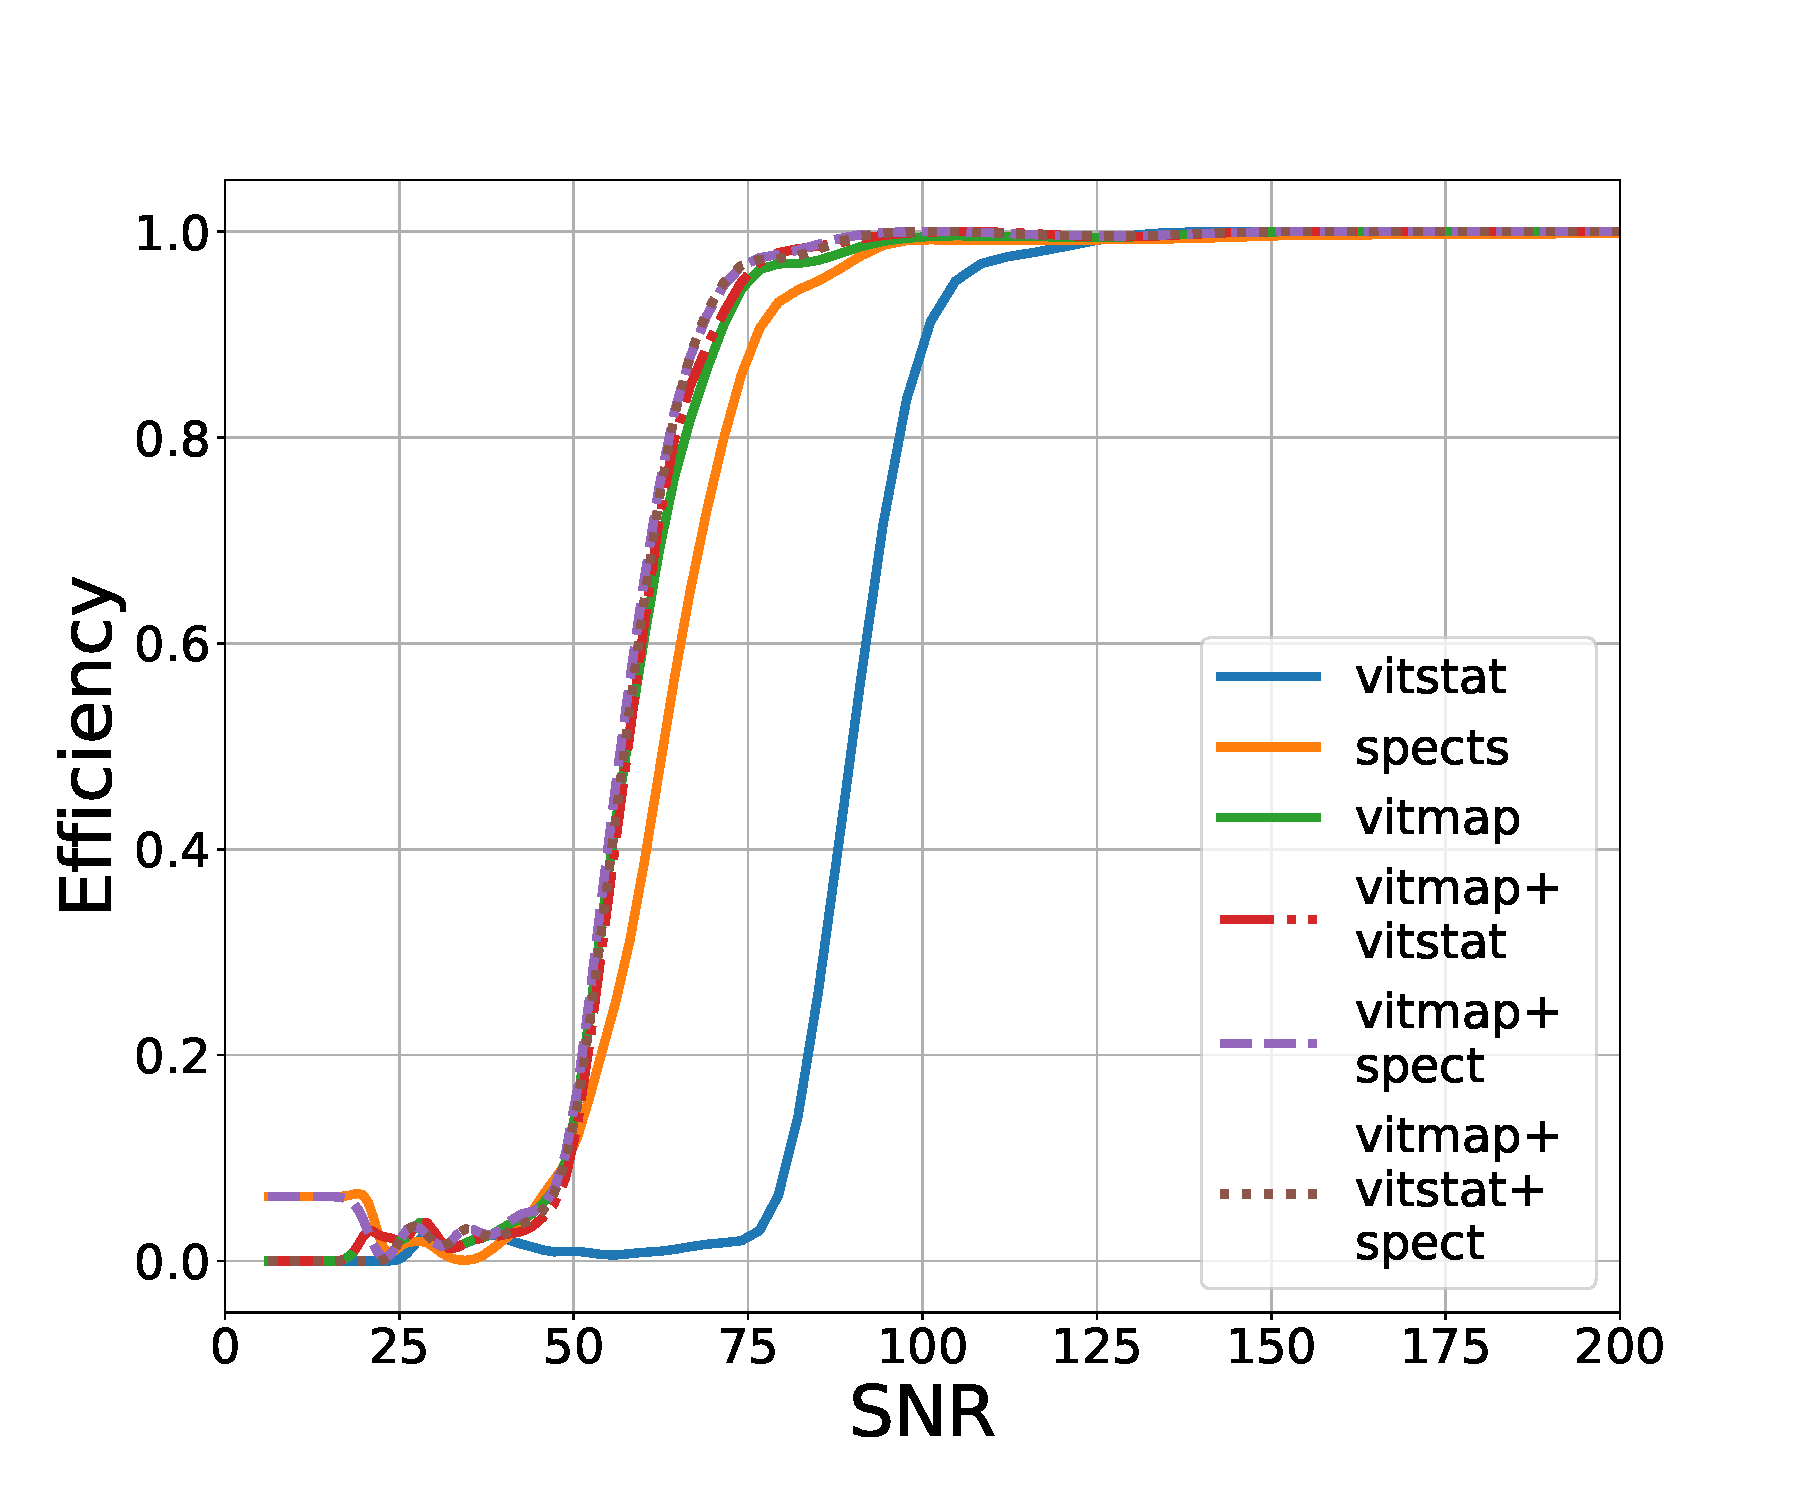
\includegraphics[width=\columnwidth]{C4_cnn/o1_snr_eff.pdf}
		\caption{\label{machine:results:snr_o1}}
	\end{subfigure}
	\begin{subfigure}[h]{0.5\textwidth}
		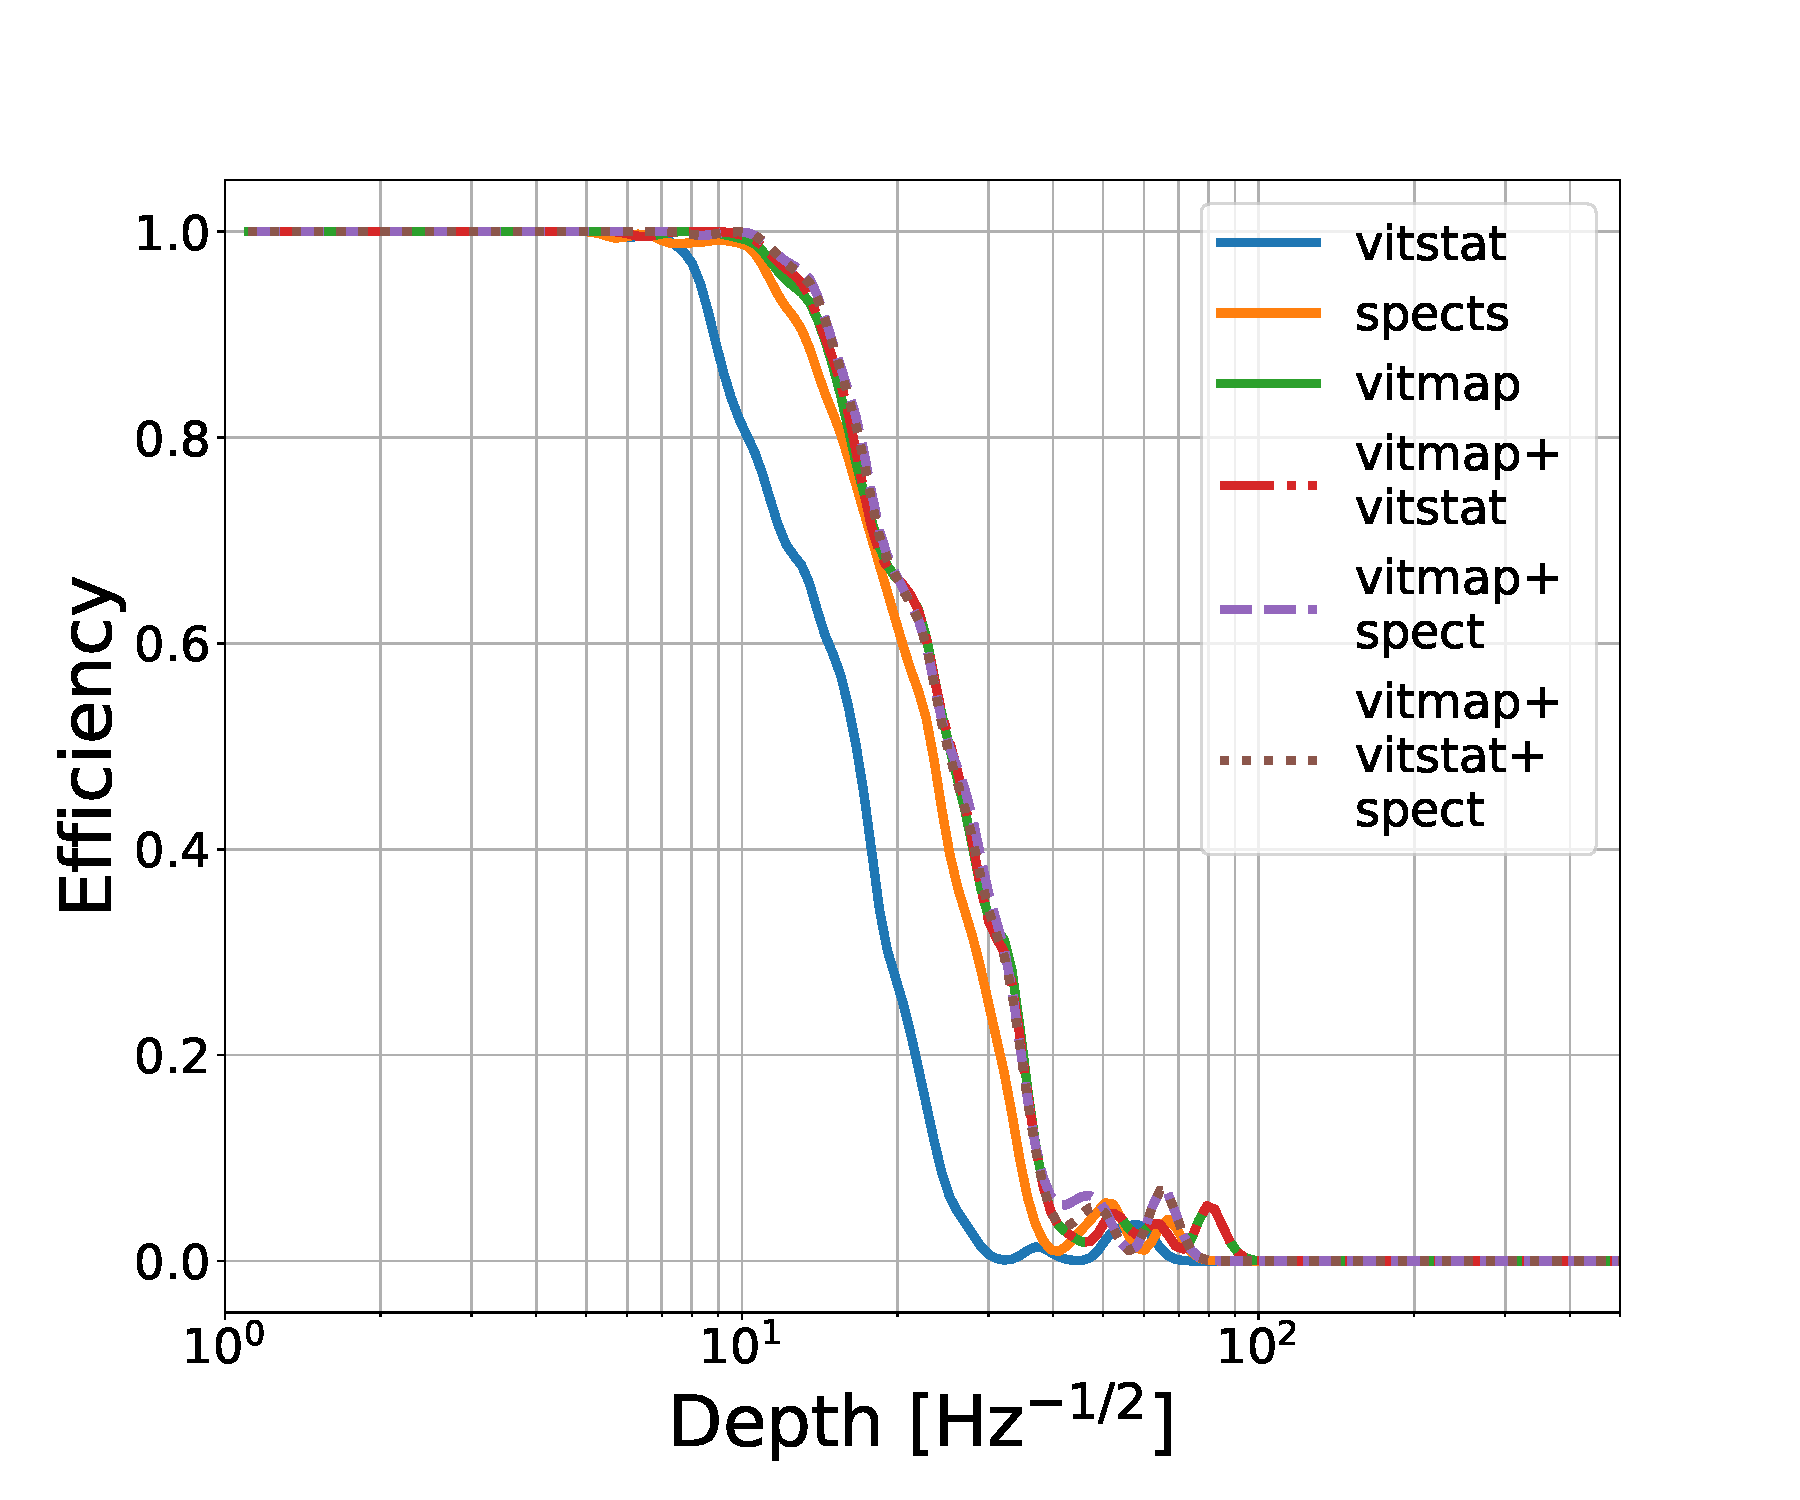
\includegraphics[width=\columnwidth]{C4_cnn/o1_depth_eff.pdf}
		\caption{}
		\label{machine:results:depth_o1}
	\end{subfigure}
	\caption[O1 results from SOAP and \gls{CNN} search.]{ In the O1 data-set, each of the six \glspl{CNN} were tested. The efficiency plots above are for a 1\% false alarm rate. }
	\label{machine:results:o1}
	
\end{figure}

%%%%%%%%%
\subsubsection{O2}
%%%%%%%%%%

% describe the first test - O2 injections
%
For the first test, injections were made into the O2 data-set as described in
Sec.~\ref{machine:data} between 100 Hz and 400 Hz. Each of the 6 networks described in
Sec.~\ref{machine:cw:structure} were then trained and tested on this data.
Figure ~\ref{machine:results:o2} shows the sensitivity curves for
this test for both \gls{SNR} and sensitivity depth for each of the 6 networks.
Focusing on Fig.~\ref{machine:results:snr_o2}, the least sensitive of the \glspl{CNN} is the
Viterbi statistic (vitstat). This is
expected as we know that the despite the line-aware aspect of the Viterbi statistic, it can still confuse some instrumental lines with an astrophysical signal. 
The spectrogram \gls{CNN} has an improved sensitivity over the Viterbi statistic,
this importantly does not involve the SOAP search but is run entirely on
down-sampled and summed spectrograms. This network is approaching the
most sensitive of the examples in Fig.~\ref{machine:results:o2}.
With further investigation involving perhaps different network structures or larger or higher resolution data sets, this could potentially reach the same sensitivity as other networks. However, this network
takes $\sim10$ times the amount of training time compared to the Viterbi map network. This
is explained in more detail in Sec.~\ref{machine:results:timing}. The
remaining four networks all achieve a similar sensitivity, each of these
networks contain the Viterbi map (vitmap) as one of their inputs or their only
input. Therefore, it is assumed that the dominating effect on the sensitivity
originated from the Viterbi maps.  In the following tests the focus
will be on the Viterbi map \gls{CNN} as in all cases this is among the most
sensitive. For the O2 data-set we show that with a false
alarm probability of 1\% the Viterbi map \gls{CNN} achieves a
sensitivity of \gls{SNR} $~95$ and sensitivity depth of $~12\; {\rm Hz}^{-1/2}$
with 95\% efficiency.
In Fig.~\ref{machine:results:snr_o2} the sensitivity of the spectrogram \gls{CNN} drops after an \gls{SNR} of 150. 
This is most likely due to the training set containing simulations between and \gls{SNR} of 50 and 150, therefore, has not seen signal simulations of higher \gls{SNR}.
The dip in sensitivity in Fig.~\ref{machine:results:depth_o2} at lower depths is from the same origin as Fig.~\ref{machine:results:snr_o2}. 


\begin{figure}
	\begin{subfigure}[h]{0.5\textwidth}
		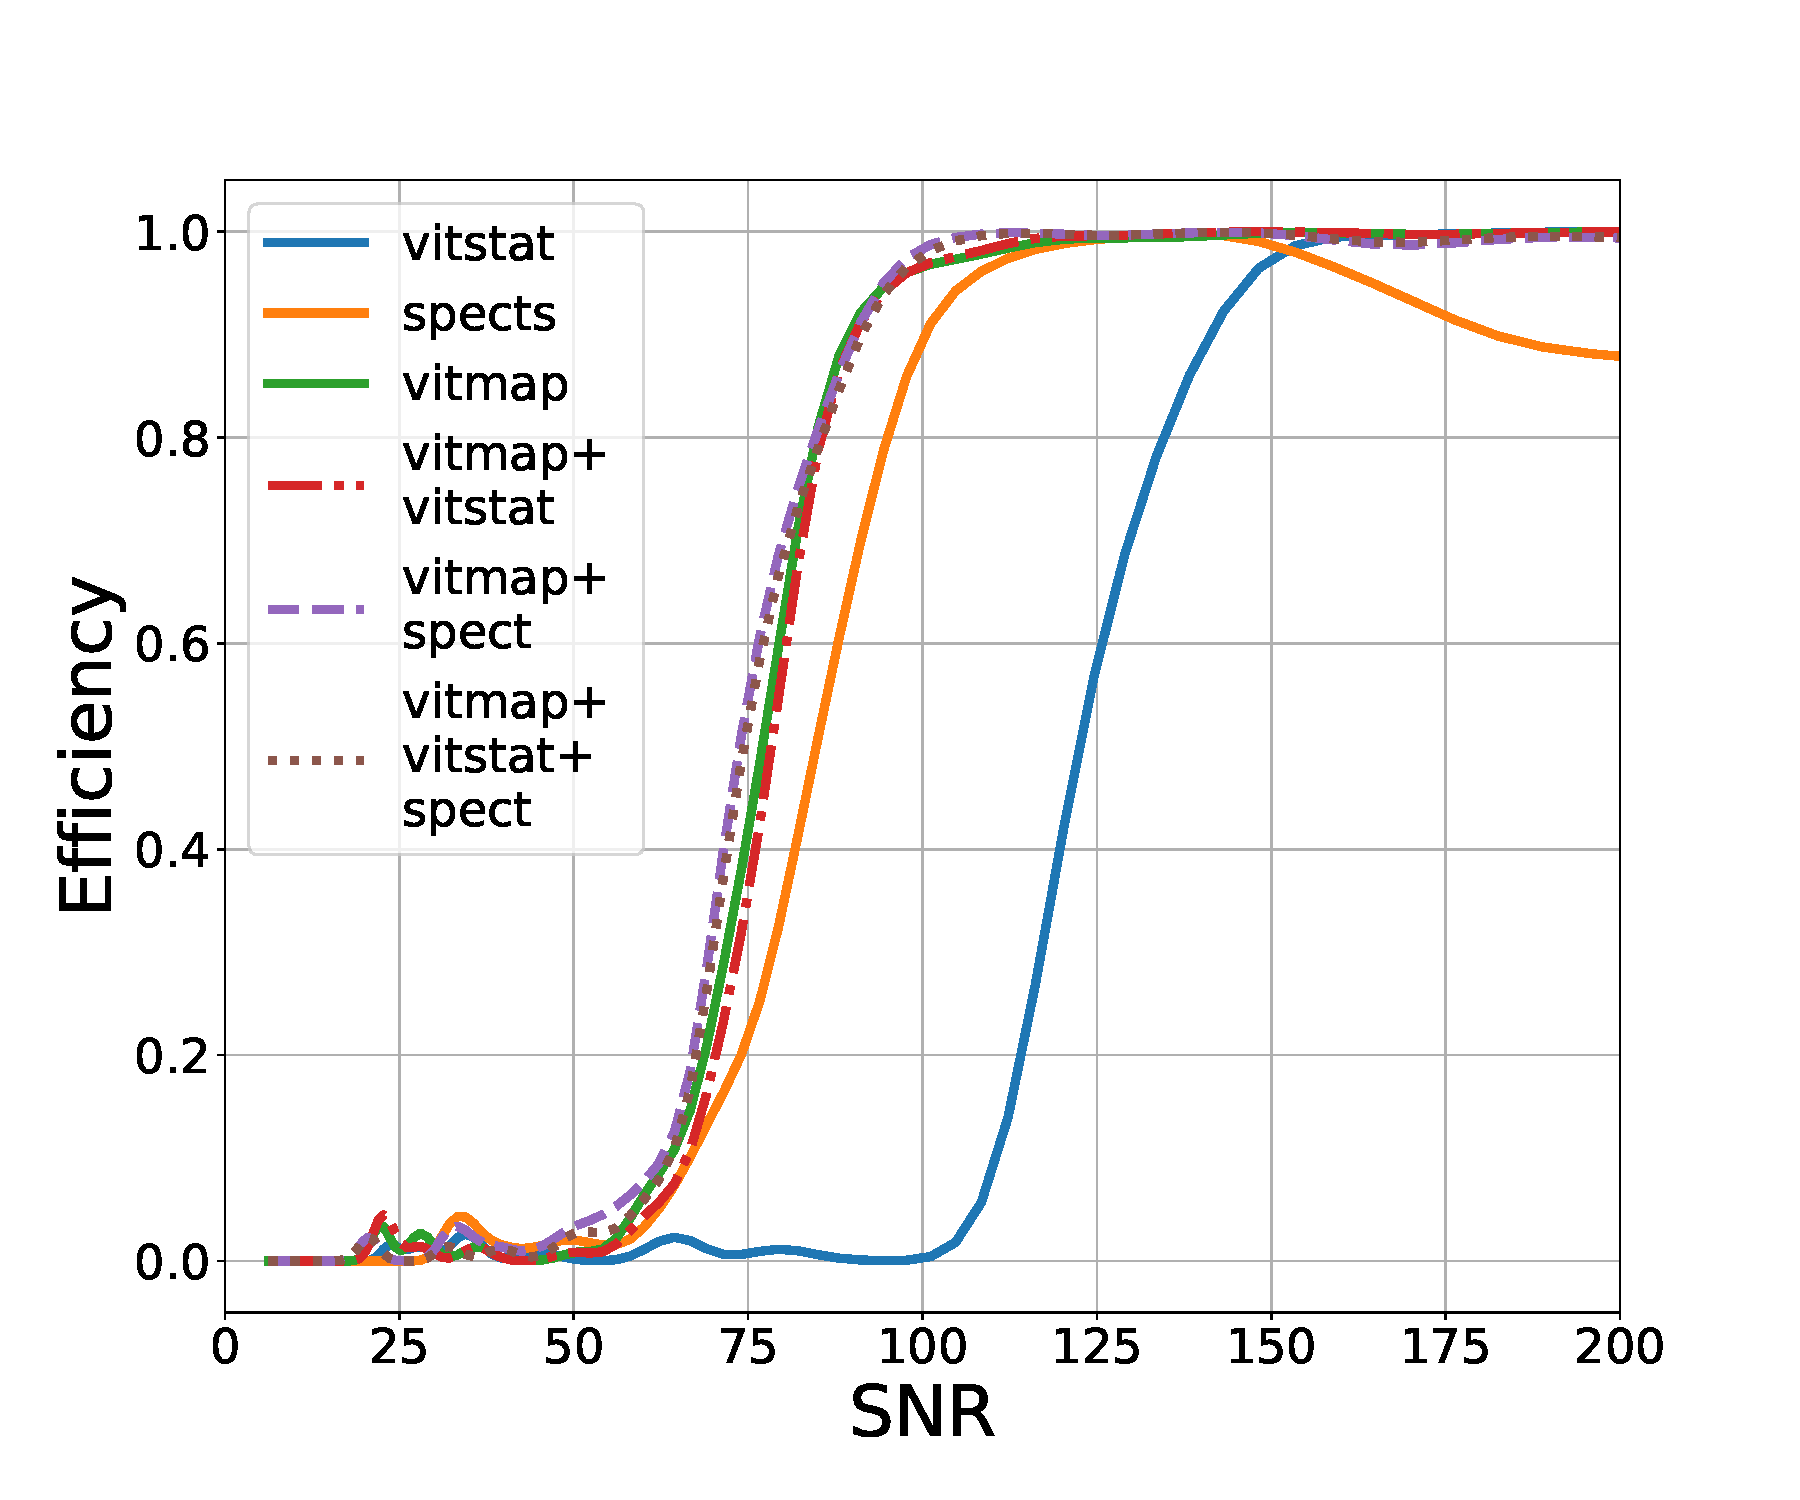
\includegraphics[width=\columnwidth]{C4_cnn/o2_snr_eff.pdf}
		\caption{}
		\label{machine:results:snr_o2}
	\end{subfigure}
	\begin{subfigure}[h]{0.5\textwidth}
		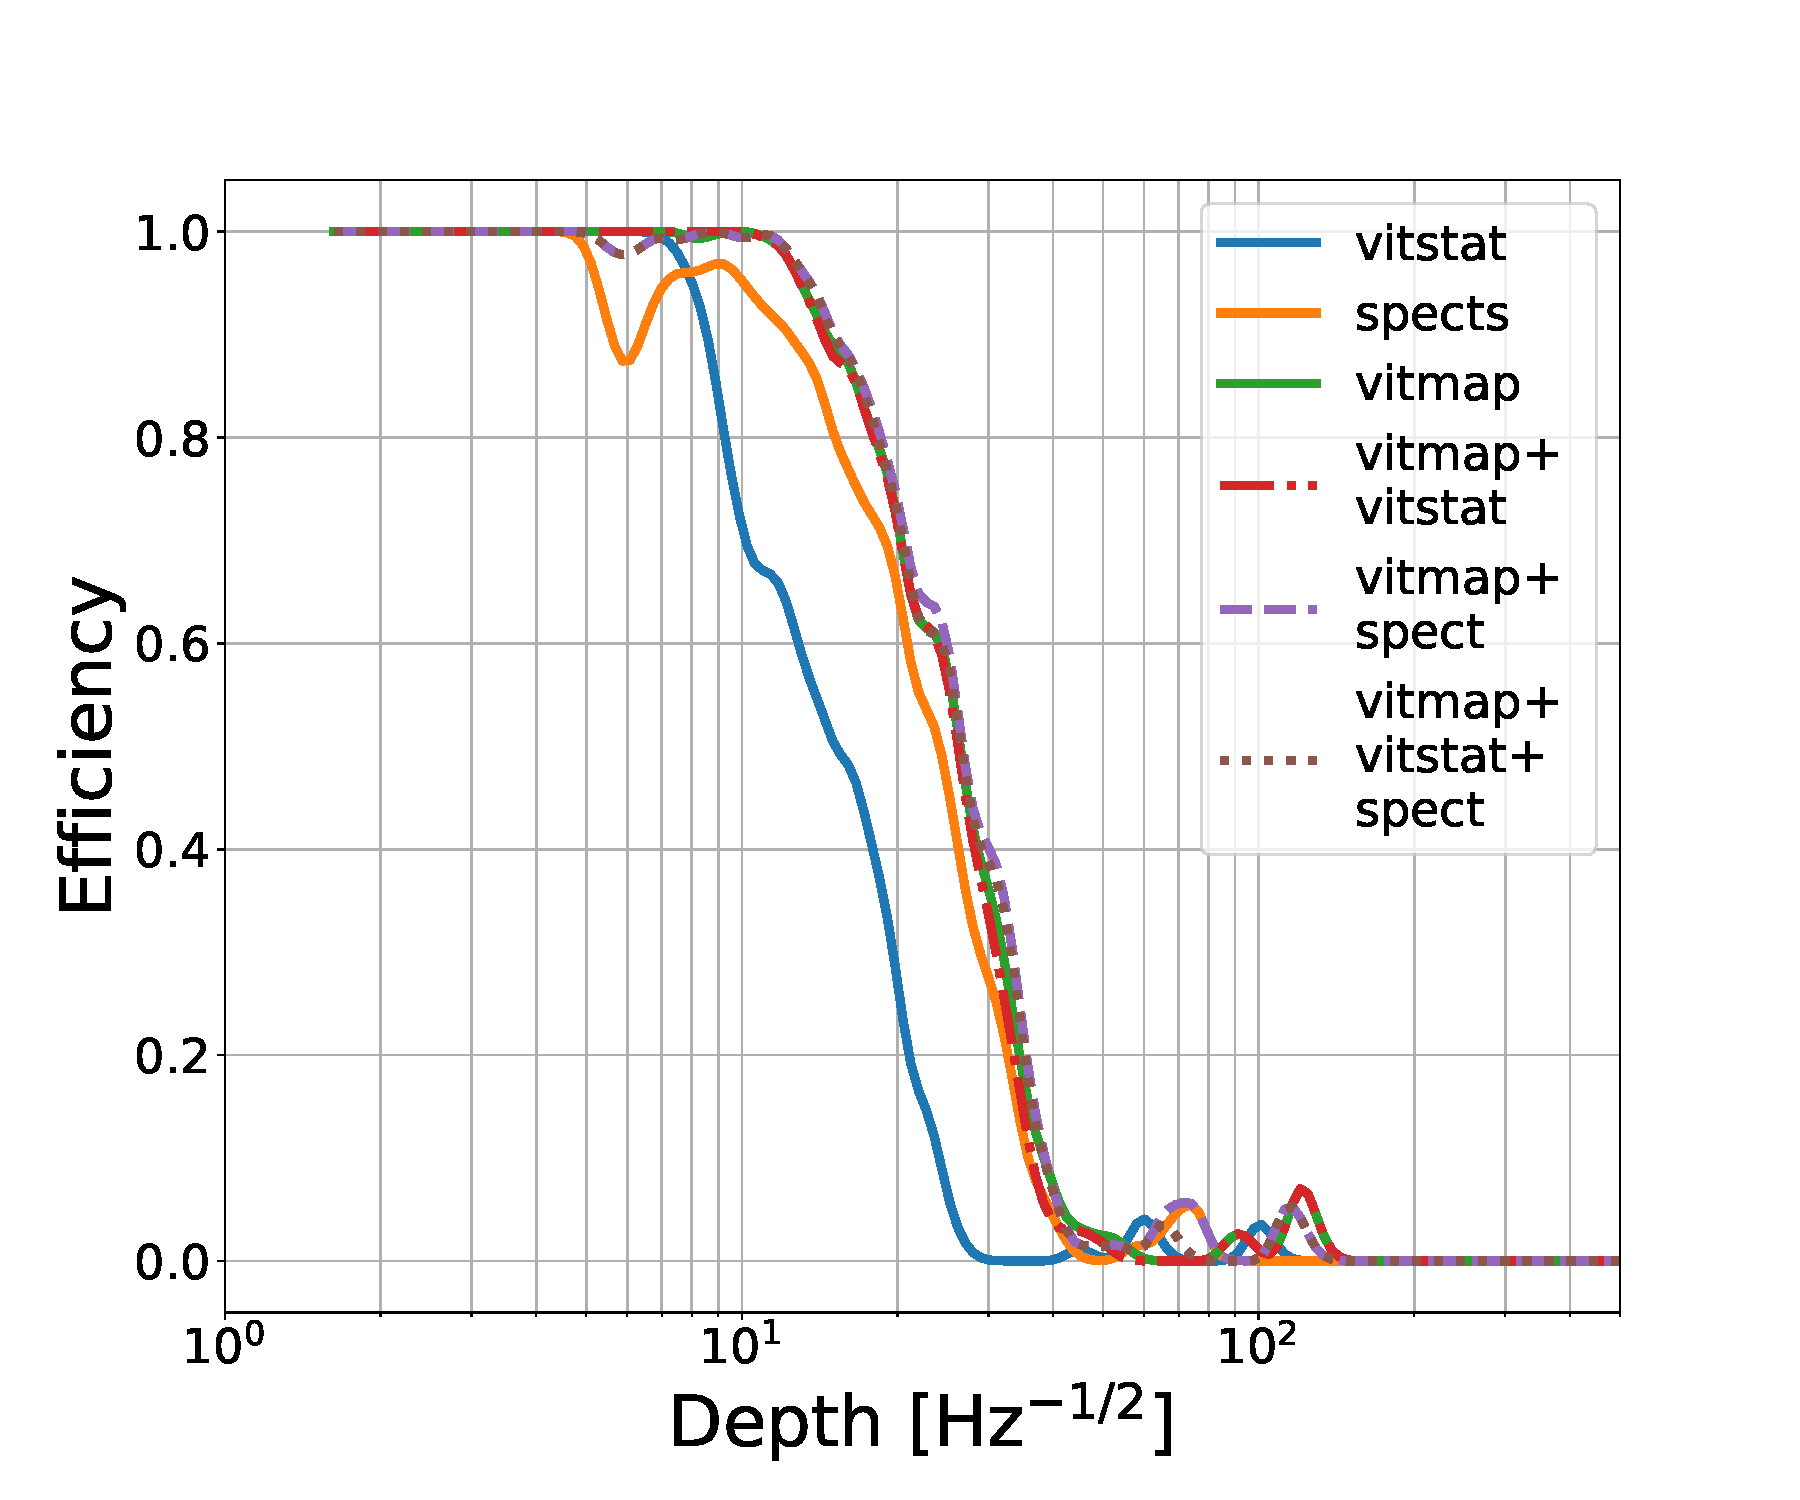
\includegraphics[width=\columnwidth]{C4_cnn/o2_depth_eff.pdf}
		\caption{}
		\label{machine:results:depth_o2}
	\end{subfigure}

	\caption[O2 results from SOAP and \gls{CNN} search.]{\label{machine:results:o2}  In the O2 data-set, each of the six \glspl{CNN} were tested. The efficiency plots above are for a 1\% false alarm rates.
	Fig.~\ref{machine:results:snr_o2} shows the efficiency of the search as a function of \gls{SNR} and Fig.\ref{machine:results:depth_o2} shows the efficiency as a function of sensitivity depth.
	The efficiency here is a measure of the fraction of events which exceed the 1\% false alarm probability for any given \gls{SNR}.
	These plots both show the sensitivity of the Viterbi statistic is far below that of the different \glspl{CNN}. 
	The others are grouped with a similar sensitivity.}
	
\end{figure}



%%%%%%%%%
\subsubsection{Gaussian noise}
%%%%%%%%%%%

% describe the second test - Gaussian noise
%
The second test involves using simulations in Gaussian noise and comparing this to simulations in S6 data.
 For this test we replicate the S6
data-set without including instrumental artefacts such as lines. We included
the same gaps in data as S6 and the noise floor of S6 was replicated by scaling
the \gls{SNR} of an injection in any given \gls{SFT} by an estimate of its \gls{PSD}. 
Figure ~\ref{machine:results:s6gauss}
shows the \gls{SNR} and depth sensitivity curves for the Viterbi statistic and Viterbi map \gls{CNN}
for both the Gaussian noise run with S6 gaps and for injections into the S6
data-set. In the Gaussian noise data-set the curves for both statistics,
Viterbi map \gls{CNN} and the Viterbi statistic, show very similar
results, this is to be expected as the main use of the \gls{CNN} was to reduce
the effect of instrumental lines, for which there are none in this data set.
The advantage of using the Viterbi maps in a \gls{CNN} becomes clear when it is
tested on simulations into real S6 data with many instrumental lines.
The two curves corresponding to simulations real S6 data in Fig.~\ref{machine:results:snr_s6} show the sensitivity as a function of \gls{SNR} in these tests. It becomes clear here that the Viterbi map \gls{CNN} reduces the effect of instrumental
lines and therefore increases the searches sensitivity to \gls{SNR}. 
A similar feature can be seen in Fig.\ref{machine:results:depth_s6} where the use of an \gls{CNN} greatly increases the sensitivity.

These tests on S6 data also show
that the effect of instrumental lines was far greater in this run than in O2.
This is shown in Fig.~\ref{machine:results:snr_o2} where the separation between the Viterbi
statistic curves and the Viterbi map curves is much smaller than the S6 curves
in Fig.~\ref{machine:results:snr_s6}. For simulations into Gaussian noise following S6
gaps we show that with a false alarm of 1\% the Viterbi map \gls{CNN} achieves a
sensitivity of SNR $~85$ and sensitivity depth of $~20\; {\rm Hz}^{-1/2}$ with
95\% efficiency. For injections into real S6 data the search achieves a
sensitivity of SNR $~115$ and sensitivity depth of $~11\; {\rm Hz}^{-1/2}$ with
95\% efficiency and 1\% false alarm. We can also see from
Fig.~\ref{machine:results:snr_s6} that the sensitivity of the vitmap \gls{CNN} in Gaussian noise with S6 gaps
is better than in real S6 data.
There are then still some artefacts in real data which reduce the sensitivity, these could potentially be non Gaussian artefacts such as weak instrumental lines.  

\begin{figure}
	\begin{subfigure}[h]{0.5\textwidth}
		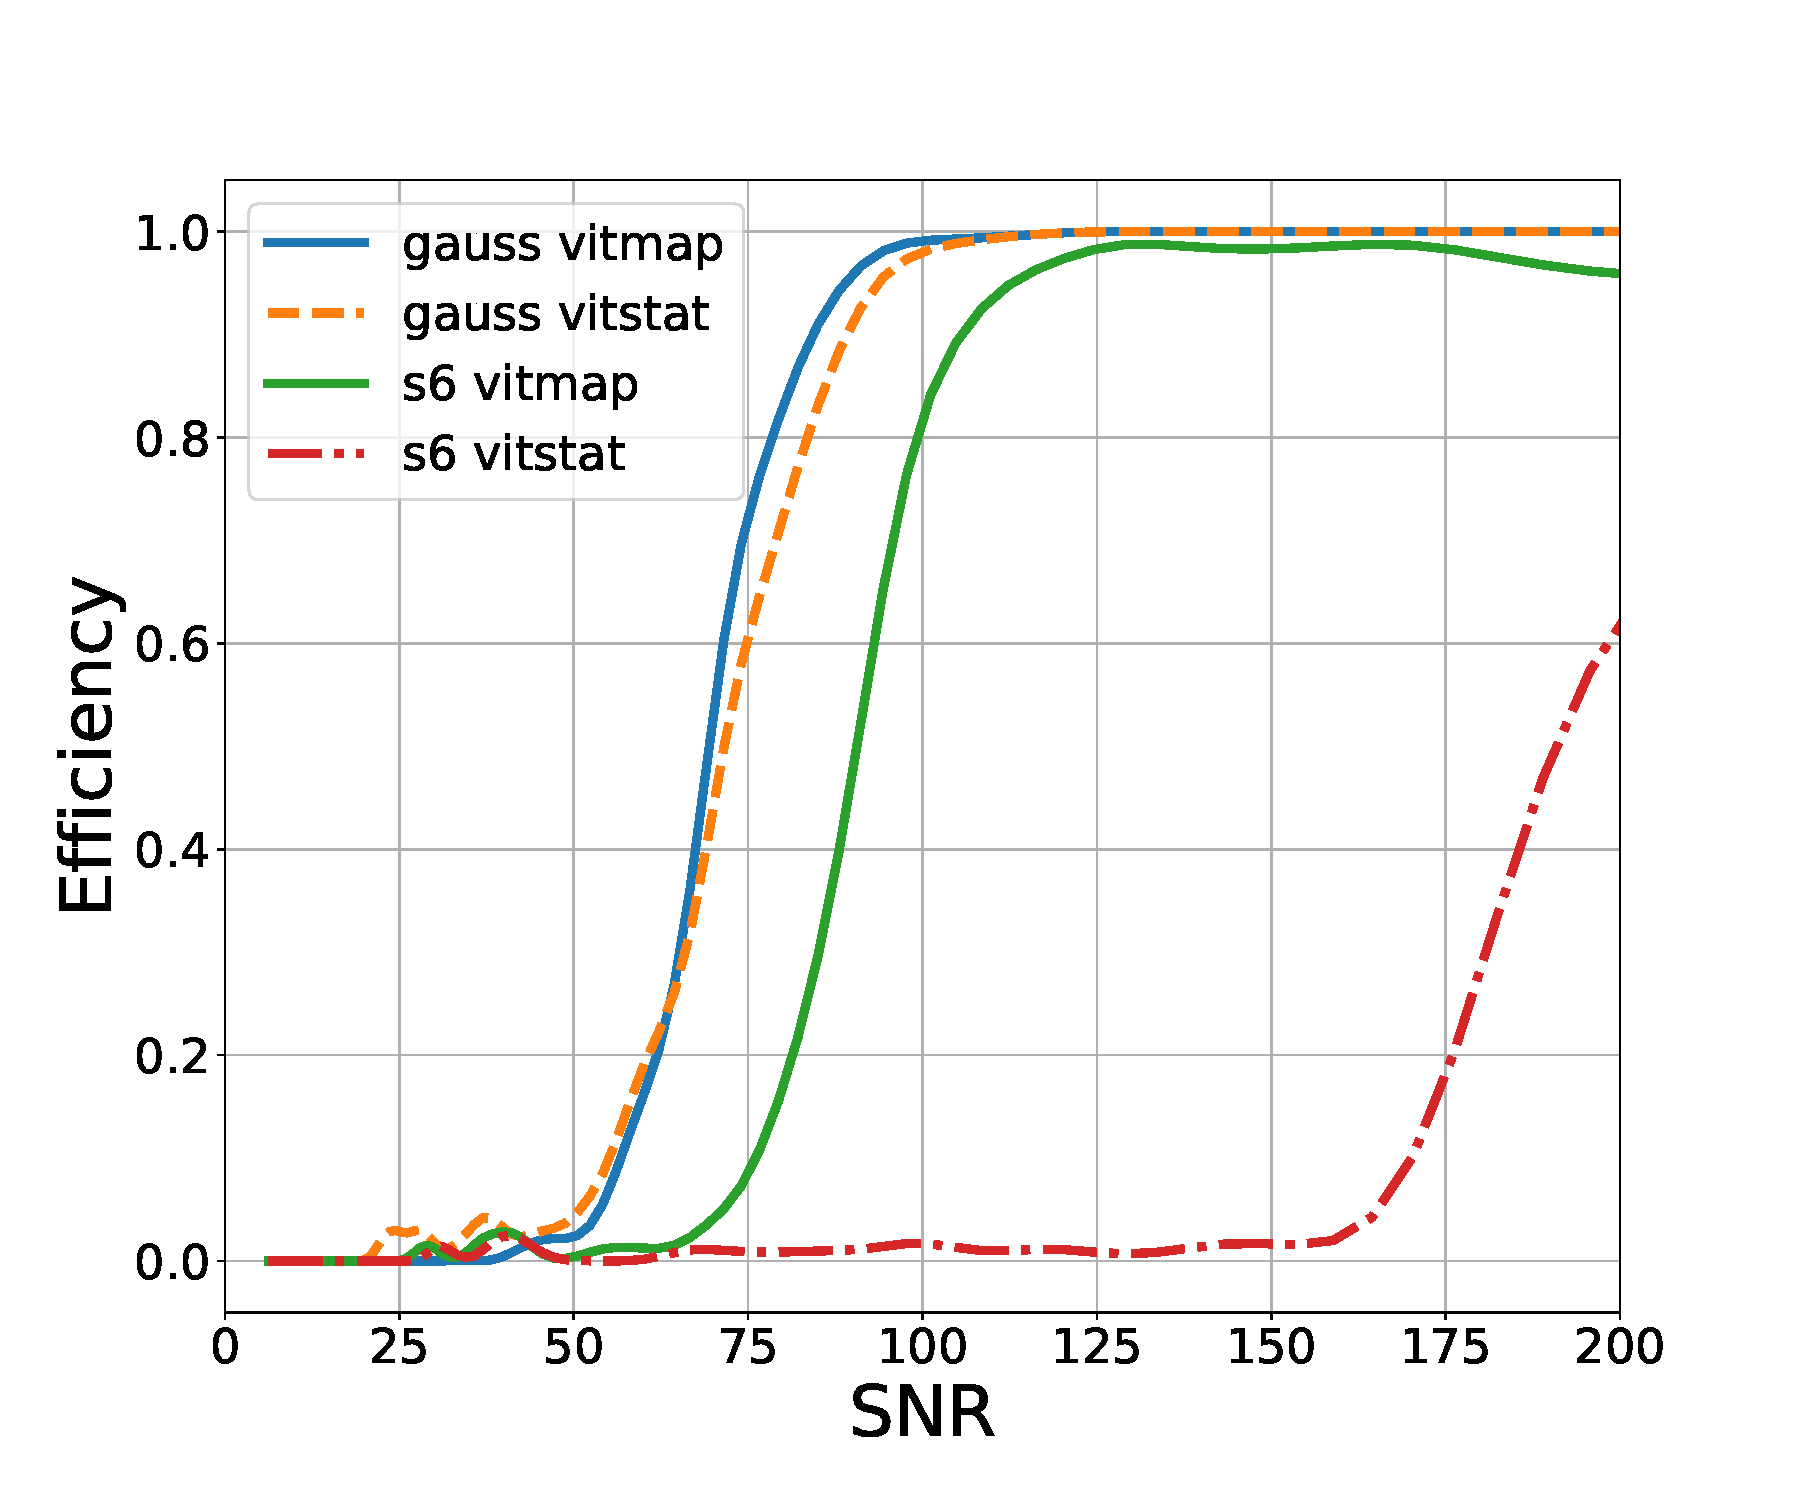
\includegraphics[width=\columnwidth]{C4_cnn/gauss_and_s6_snr_eff.pdf}
		\caption{}
		\label{machine:results:snr_s6}
	\end{subfigure}
	\begin{subfigure}[h]{0.5\textwidth}
		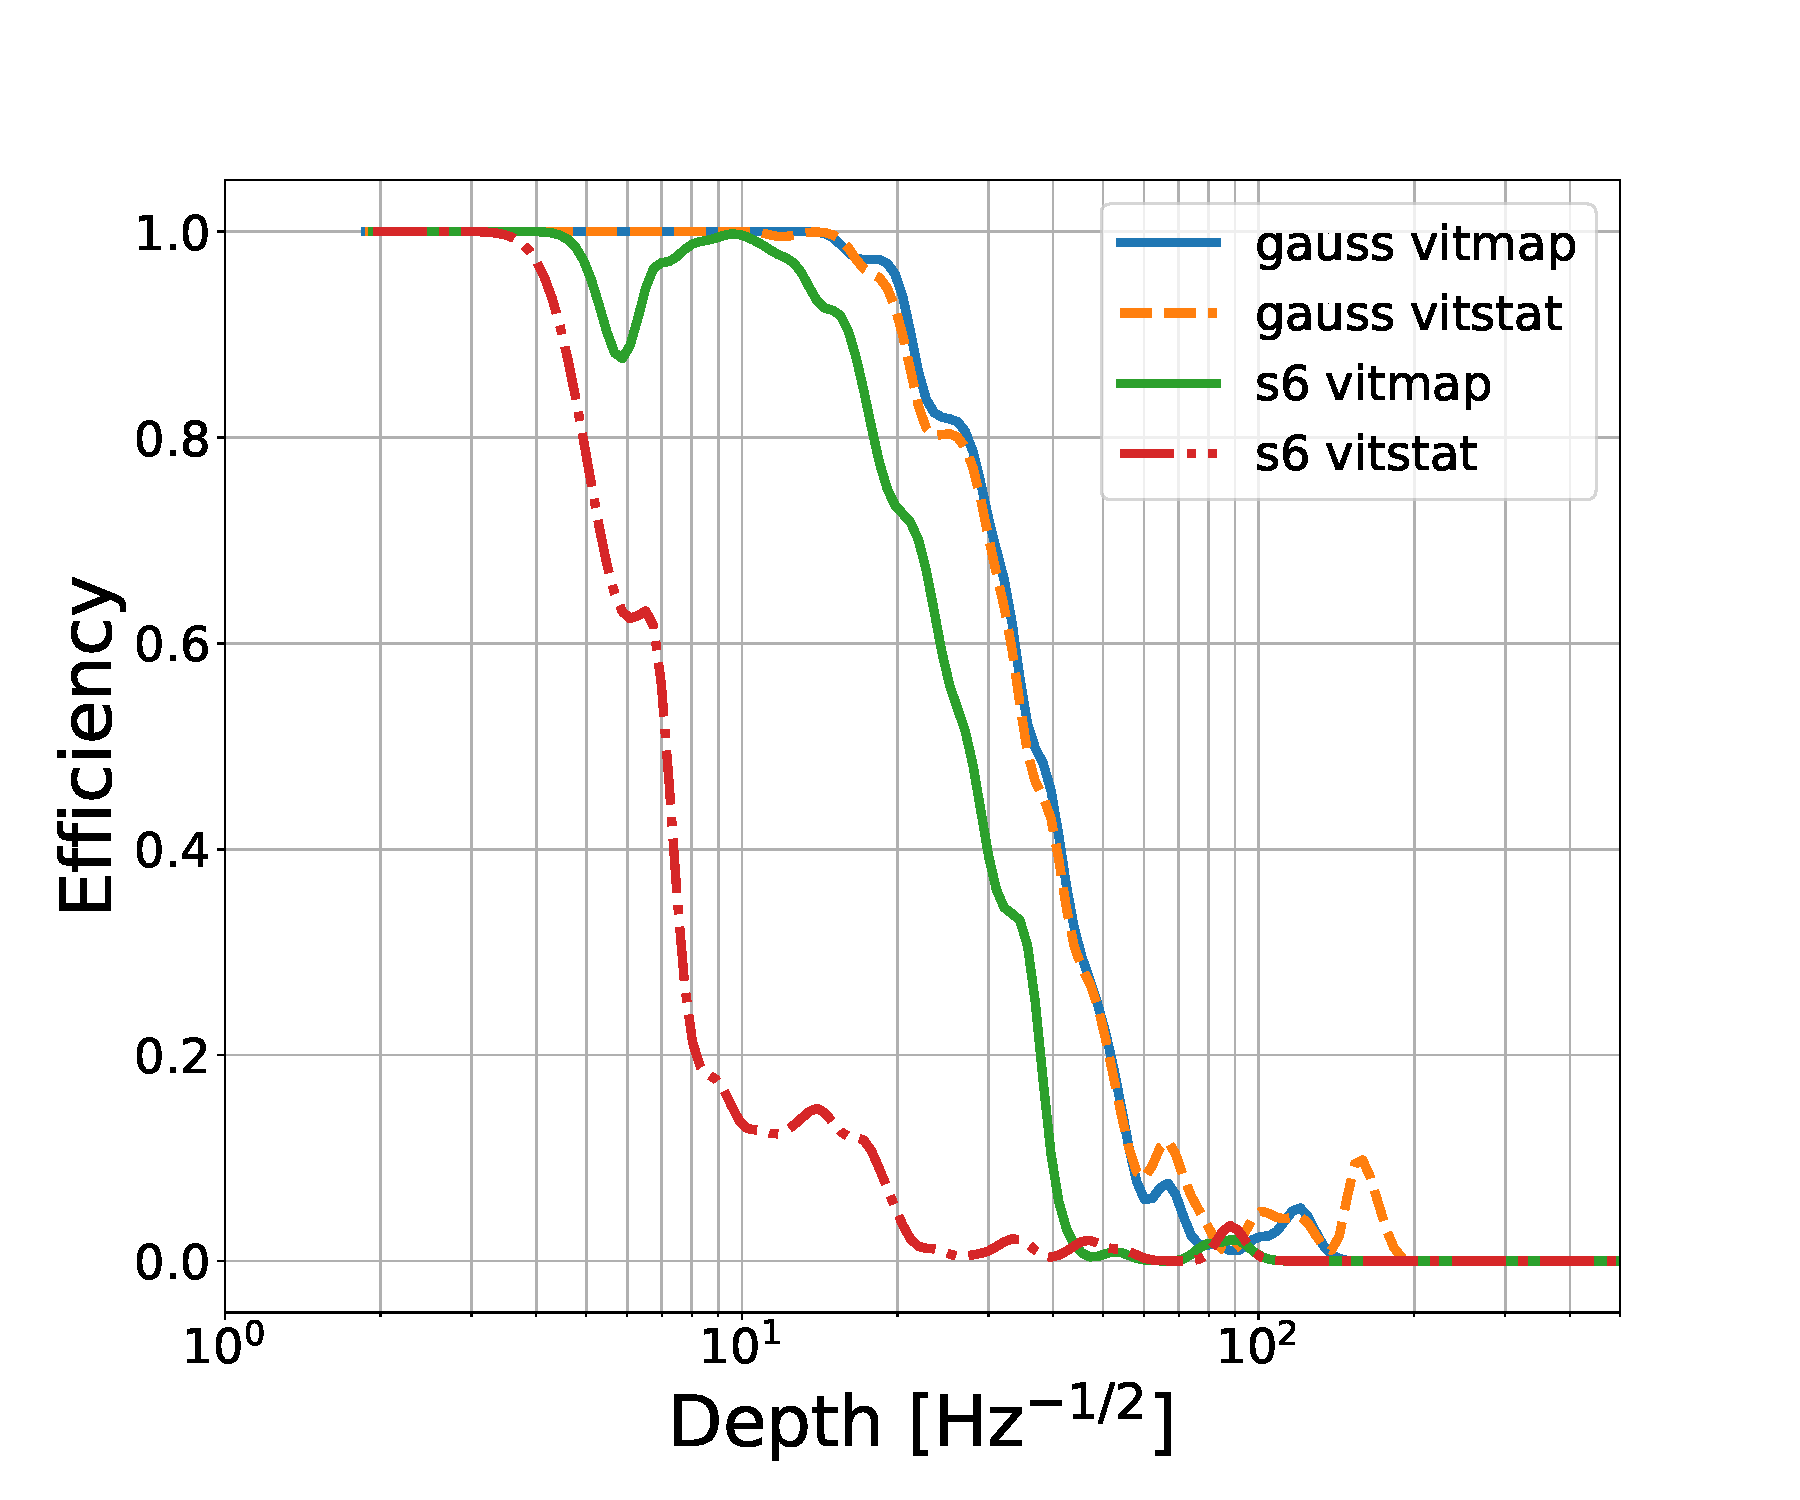
\includegraphics[width=\columnwidth]{C4_cnn/gauss_and_s6_depth_eff.pdf}
		\caption{}
		\label{machine:results:depth_s6}
	\end{subfigure}

	\caption[Gaussian noise results from SOAP and \gls{CNN} search.]{\label{machine:results:s6gauss} We compared the sensitivity of this
	search on simulations on real S6 data (s6) to simulations in Gaussian noise
	(gauss). Figure \ref{machine:results:snr_s6} shows the efficiency of the search as a function of \gls{SNR} and Fig.~\ref{machine:results:depth_s6} shows the efficiency as a function of sensitivity depth.
	The efficiency is the fraction of events which exceed the 1\% false alarm threshold for a given \gls{SNR} or depth.
	The Gaussian noise injections included the same gaps in data as the S6
	data set. The \gls{SNR} of the simulated signal in Gaussian noise was adjusted
	based on the noise floor of S6. 
	In the Gaussian noise simulations the searches achieve an efficiency of $90\%$ with 1\% false alarm at an \gls{SNR} $\sim 85$ and $\sim 90$ for the Viterbi map and Viterbi statistic respectively.
	In the real S6 noise simulations the searches achieve an efficiency of $90\%$ with 1\% false alarm at an \gls{SNR} $\sim 108$ and $ > 200$ for the Viterbi map and Viterbi statistic respectively.}
	
\end{figure}


%%%%%%%
\subsubsection{S6}
%%%%%%%%%%

% the 3rd test - S6 MDC comparison
%
The final test was set up to again use the S6 data-set, however, in this case
we use a standard set of injections in the S6
\gls{MDC}~\citep{walsh2016ComparisonMethods} to compare directly to other \gls{CW}
search pipelines. In Fig.~\ref{machine:results:s6mdc} we show the results of the
sensitivity curves from these injections. 
In both Fig.~\ref{machine:results:snr_s6mdc} and \ref{machine:results:depth_s6mdc} the sensitivity curves are substantially more noisy than in Fig.~\ref{machine:results:o2} or \ref{machine:results:s6gauss}, this is mainly due to the size of the testing set.
The standard set of simulations in Fig.~\ref{machine:results:s6mdc} contained $\sim 900$ signal simulations between 40 and 500 Hz where the majority of these signals are distributed between an \gls{SNR} of 0 and 150. 
Figures \ref{machine:results:o2} and \ref{machine:results:s6gauss} are generated using $2300$ simulations between 40 and 500 Hz and \glspl{SNR} of 20 and 200 as described in Sec.~\ref{machine:pipeline}.
Figure ~\ref{machine:results:depth_s6mdc} shows the direct comparison in depth of the
results in~\citep{walsh2016ComparisonMethods} with the results from the SOAP
search with the Viterbi map \gls{CNN}. This shows that we achieve a sensitivity
consistent with that of other semi-coherent searches with the
exception of the Einstein@home search~\citep{abbott2016ResultsDeepest}. Whilst
we are not at the most sensitive end of these searches, the SOAP and \gls{CNN}
search offers a greatly reduced computational cost. This will be explained in more detail in
Sec.~\ref{machine:results:timing}. This particular test was limited to searching for
isolated neutron stars, however, unlike some other semi-coherent searches such as Einstein@Home \citep{singh2016ResultsAllsky} or the time domain $\mathcal{F}$-statistic \citep{aasi2014ImplementationTextdollar}, SOAP has a lot of flexibility in the type of signal which it can search for.
The inclusion of the \gls{CNN} does introduce some dependency of the search
on the model as the training set for the \gls{CNN} contained simulations of isolated pulsars. 
However, this is not a limitation of the method but of the training set as, for example, a new training set using a different signal model could be generated. 
For tests in the S6 \gls{MDC} we show that with a false alarm of 1\% the Viterbi map
\gls{CNN} achieves a sensitivity in SNR of $\sim 90$ and sensitivity depth of
$\sim 16\;{\rm Hz}^{-1/2}$ with 95\% efficiency.


\begin{figure}
	\begin{subfigure}[h]{0.5\textwidth}
		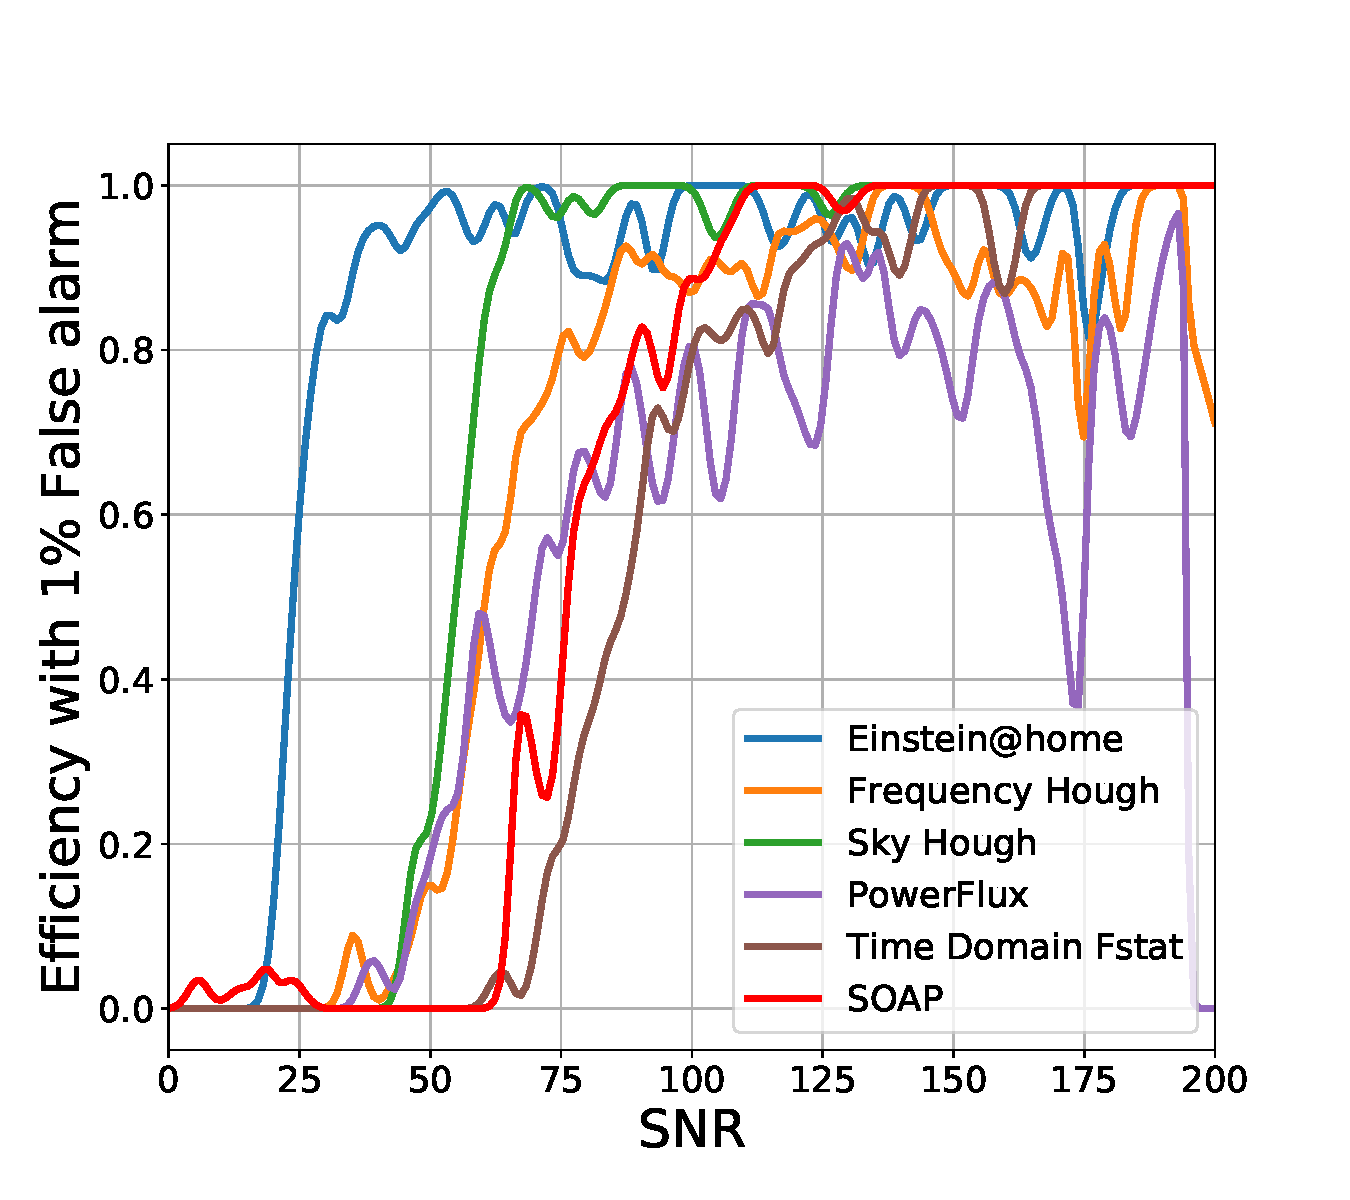
\includegraphics[width=\columnwidth]{C4_cnn/S6MDC_snr.pdf}
		\label{machine:results:snr_s6mdc}
	\end{subfigure}
\begin{subfigure}[h]{0.5\textwidth}
	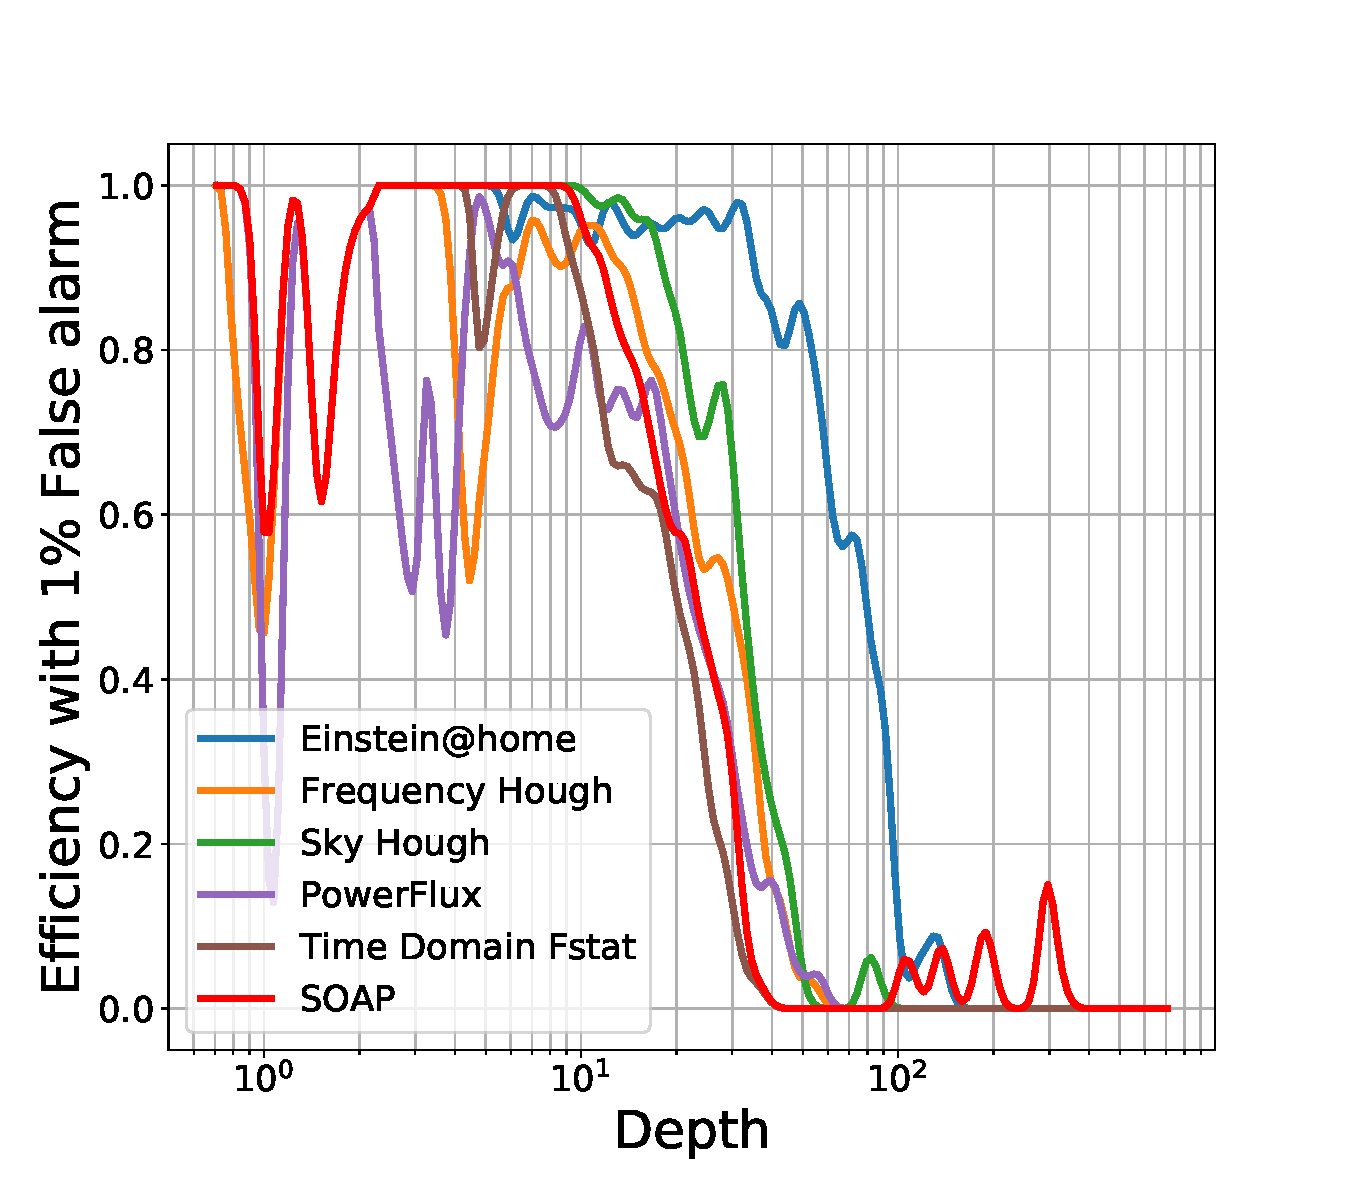
\includegraphics[width=\columnwidth]{C4_cnn/S6MDC_depth.pdf}
	\label{machine:results:mdccomp}
\end{subfigure}

	\caption[S6 \gls{MDC} results from SOAP and \gls{CNN} search.]{\label{machine:results:s6mdc} To compare the SOAP and \gls{CNN} search to other existing \gls{CW} searches, we used a standard set of injections used in the S6 \gls{MDC} \citep{walsh2016ComparisonMethods}.
	We have taken the list of detected pulsars for each search
	from this paper \citep{walsh2016ComparisonMethods} and replotted using the
	method in Sec.~\ref{machine:results:sensitivity} to compare the sensitivities to the SOAP + \gls{CNN} search. 
	This includes results for all pulsar simulations between 40 and 500 Hz. 
	The efficiency curves are generated with a 1\% false alarm probability. }
	
\end{figure}

%%%%%
\subsection{\label{machine:results:timing} Computational time}
%%%%


A key property of any \gls{CW} search is the computational
time taken for the search to run. 
Table \ref{timing:table} shows the timings for different sections of the search when run on the S6 dataset. 
This can be split into three main sections: data generation, \gls{CNN} training and \gls{CNN} testing.
To get from raw \glspl{SFT} to results with this search, the majority of the computational time taken is in the data generation step.
The timings shown Tab.~\ref{timing:table} are for the S6 observing run where each section is run on a single \gls{CPU} or \gls{GPU}, however, in practice the generation of the data is generally run on multiple \glspl{CPU} on a computing cluster.
The training and testing of a \gls{CNN} is done on a single\gls{GPU}, this substantially decreases the training time compared to a \gls{CPU} due to the parallel nature of neural networks. 


\begin{table}
%                                                                                                                 
\caption{\label{timing:table}
The approximate timings were measured for each part of the search. This table shows the timings for training and testing starting from raw \glspl{SFT}. This is the results from S6 which is the longest run we tested. We used S6 data in the frequency range
between 40-500 Hz and it had a length 22538 \glspl{SFT} with time base of 1800 s. In the training,testing and search data sections we averaged the \glspl{SFT} over one day such that we had 469 time segments as input to the \glspl{CNN}. The data generation times here are for a single \gls{CPU} however, in reality this will be split across many separate \glspl{CPU}. The training and testing is completed on a single \gls{GPU}.}

%   
\centering
\bgroup
\def\arraystretch{1.5}
\centering
\begin{tabular}{c c c}
 \multicolumn{3}{c}{{\bf Generating data on single \gls{CPU}}}  \\
\hline
\hline
 & \multicolumn{2}{c}{Time [hrs]} \\
\hline
Narrow-banding & \multicolumn{2}{c}{$\sim 9$}   \\
\hline
Training data& \multicolumn{2}{c}{$\sim 240$} \\
\hline
Testing data& \multicolumn{2}{c}{$\sim 75$}  \\
\hline
Search data& \multicolumn{2}{c}{$\sim 40$}  \\
\hline
\hline
 \multicolumn{3}{c}{{\bf Training \glspl{CNN} on single \gls{GPU}} }  \\
\hline
\hline
 & Training time [hrs] & Loading time [hrs]\\
\hline
Viterbi statistic & $0.03$ & $0.2$ \\
\hline
Viterbi map & $0.8$ & $0.7$ \\
\hline
spectrogram & $9$ & $1$\\
\hline
Viterbi map \\ + Viterbi statistic& $1$ &$0.7$ \\
\hline
Viterbi map \\ + spectrogram& $1.4$ & $1.6$\\
\hline
Viterbi map \\ + Viterbi statistic \\ + spectrogram& $1.5$ & $2$ \\
\hline
\hline
 \multicolumn{3}{c}{{\bf Testing \glspl{CNN} on real data on \gls{GPU}}}  \\
 \hline
 \hline
 & Testing [s] & Loading [s] \\
\hline
 All \glspl{CNN} & $5$ & $60-160$ \\
\hline
\hline
\end{tabular}
\egroup
\end{table}

% conclusions to be drawn from the table of timings
%
One can start from raw \glspl{SFT} from the S6 dataset without any trained networks, where this dataset has 22538, 1800 s long \glspl{SFT} and we search between 40-500 Hz, i.e. 828000 frequency bins. 
This search would have a total computing time of $ \sim 386$ hours on a single \gls{CPU} and \gls{GPU}.
However, the majority of this time is taken generating the appropriate data.
The generation of training, testing and search data can be easily parallelised, where in practice this is split over 200 \glspl{CPU} so that it takes $\sim 2$ hours instead of $\sim 355$ hours. 
Rather than taking $\sim 364$ hours, the generating data section then takes $\sim 11$ hours in real time.
After this parallelisation, if one was given S6 data without any trained networks, the search would then take approximately $13$ hours to get an efficiency curve and a list of candidates. In this case I assume that only the Viterbi map network is trained and tested based on the conclusions from Sec.~\ref{machine:results}. 

The computational cost could be reduced further if a network had been trained on a previous observing run. 
This would mean that the generating of the training data and the training of the network may not be needed.
This would reduce the total run time on S6 to $\sim 9.5$ hours. 
However, this does not drastically reduce the run time as the majority of the time is spent narrow-banding the \glspl{SFT} which is not run in parallel.

To reduce the time taken to generate results at the end of an observing run, one could narrowband the \glspl{SFT} periodically as the data is taken during an observing run. 
This would allow the results to be generated within $\sim 3.5$ hours of the end of the run.
\glspl{SFT} generated on a regular basis would allow results to be generated during an observing run.
This could be done, for example, on a weekly basis by adding 7 days of pixels to a spectrogram, then retraining a \gls{CNN} and generating results.

The computational cost of this search is small when compared to other existing \gls{CW} searches. In \cite{walsh2016ComparisonMethods} the expected computational cost for the first 4 months of O1 for each search is shown, where the fastest search takes $0.9$ million core-hours (Hough searches) and the slowest is $100-170$ million core-hours (Einstein@Home).
The equivalent cost of the SOAP + \gls{CNN} search is $\sim 100-200$ core-hours which is $\sim 5-10$ thousand times faster.

\clearpage

%%%%%
%%%%%
\section{\label{machine:results:sens_size} Sensitivity with the size of dataset}
%%%%%
%%%%%

When training a \gls{CNN}, the general rule is that the more data the better. 
More data can limit effects such as over-training mentioned in Sec.~\ref{machine:training}, and can increase the \glspl{CNN} sensitivity.
To investigate how the sensitivity of the search changes with the number of training examples, the Viterbi map (vitmap) network in Sec.\ref{machine:results} was trained using a range of sizes of the training set. 
These networks are then tested on a separate dataset of a fixed size to see how they perform.
This was repeated for two data-sets: \gls{CW} simulations in Gaussian noise and simulations in \glspl{LIGO} O1 data-set. 
For both of these cases six different networks were trained, these used: 100, 500, 1000, 5000, 10000 and 15000 Viterbi maps as their training datasets.
Each of these different sizes of training data is a randomly selected subset of the training data used in Sec.~\ref{machine:results:sensitivity}.
The test data for each was the same entire tests sets as in Sec.~\ref{machine:results:sensitivity}.

Figure \ref{machine:results:sens_size:gauss_sens:eff} shows that in the Gaussian noise case, the majority of the networks performed with approximately the same sensitivity. 
This is with the exception of the network which was trained with 100 input Viterbi maps. 
Figure \ref{machine:results:sens_size:gauss_sens:train} shows that the sensitivity does appear to decrease, however, this is only by an \gls{SNR} of $\sim 5$.
The implication of this is that the information in the Viterbi maps is relatively easy to extract when simulations are in Gaussian noise. 
In this case the network is trying to distinguish Gaussian noise from a simulated \gls{CW} signal.
Therefore, one would expect this to be an easier problem for the network to solve compared to trying to distinguish an \gls{CW} signal from instrumental lines and Gaussian noise. 

\begin{figure}[h]
	\begin{subfigure}[h]{0.5\textwidth}
		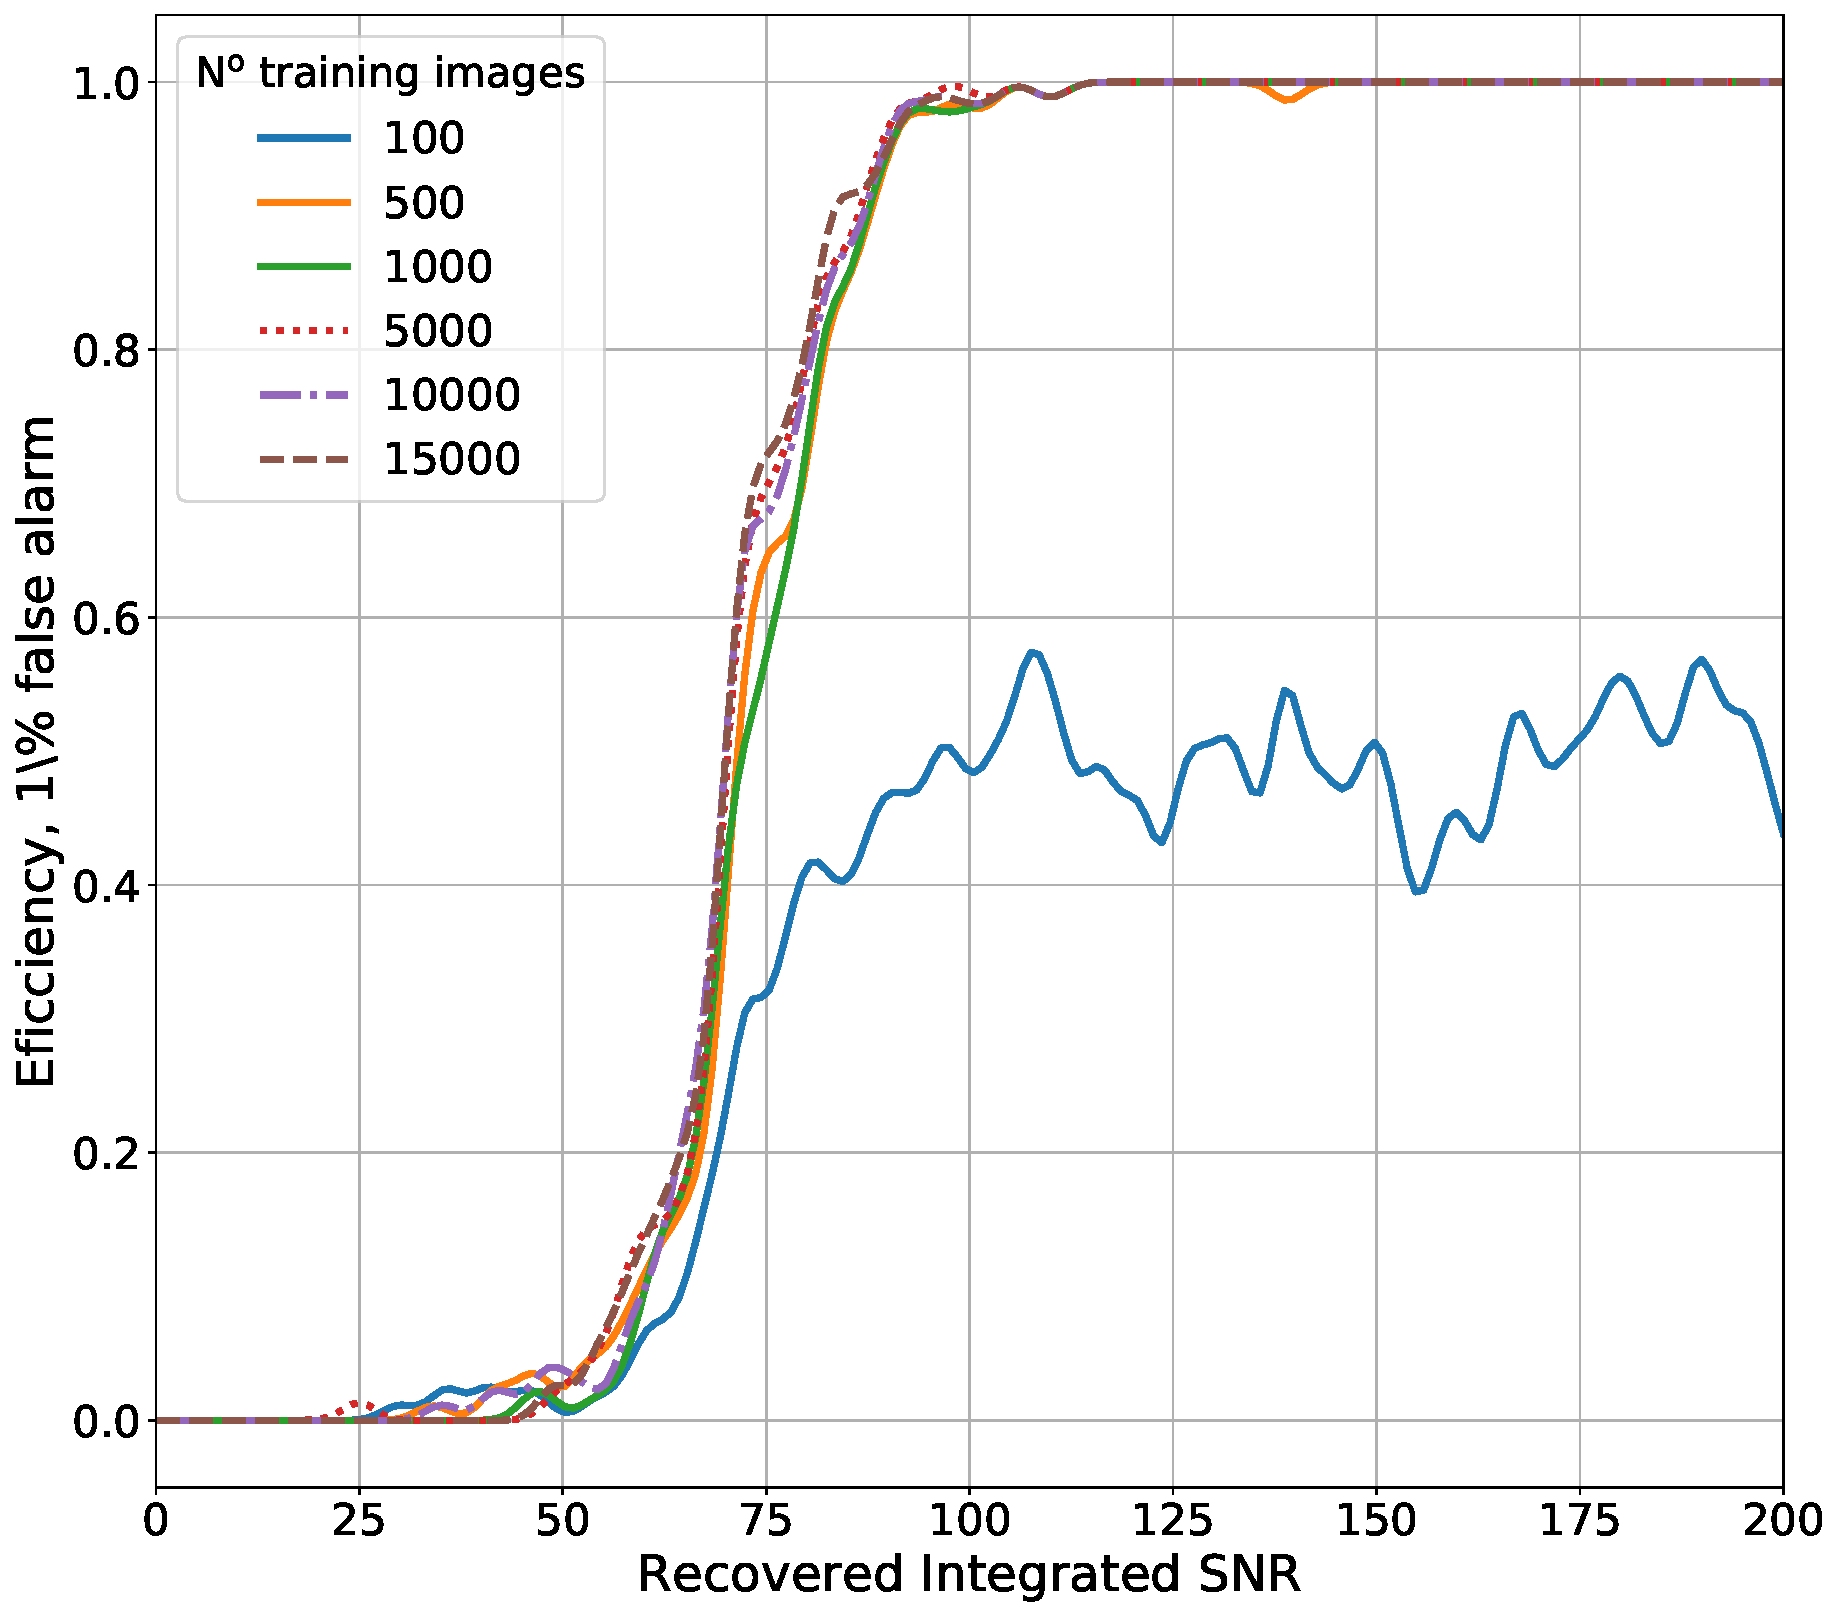
\includegraphics[width=\linewidth]{C4_cnn/gauss_sens_with_trainnum_eff.pdf}
		\caption{}
		\label{machine:results:sens_size:gauss_sens:eff}
	\end{subfigure}
	\begin{subfigure}[h]{0.5\textwidth}
		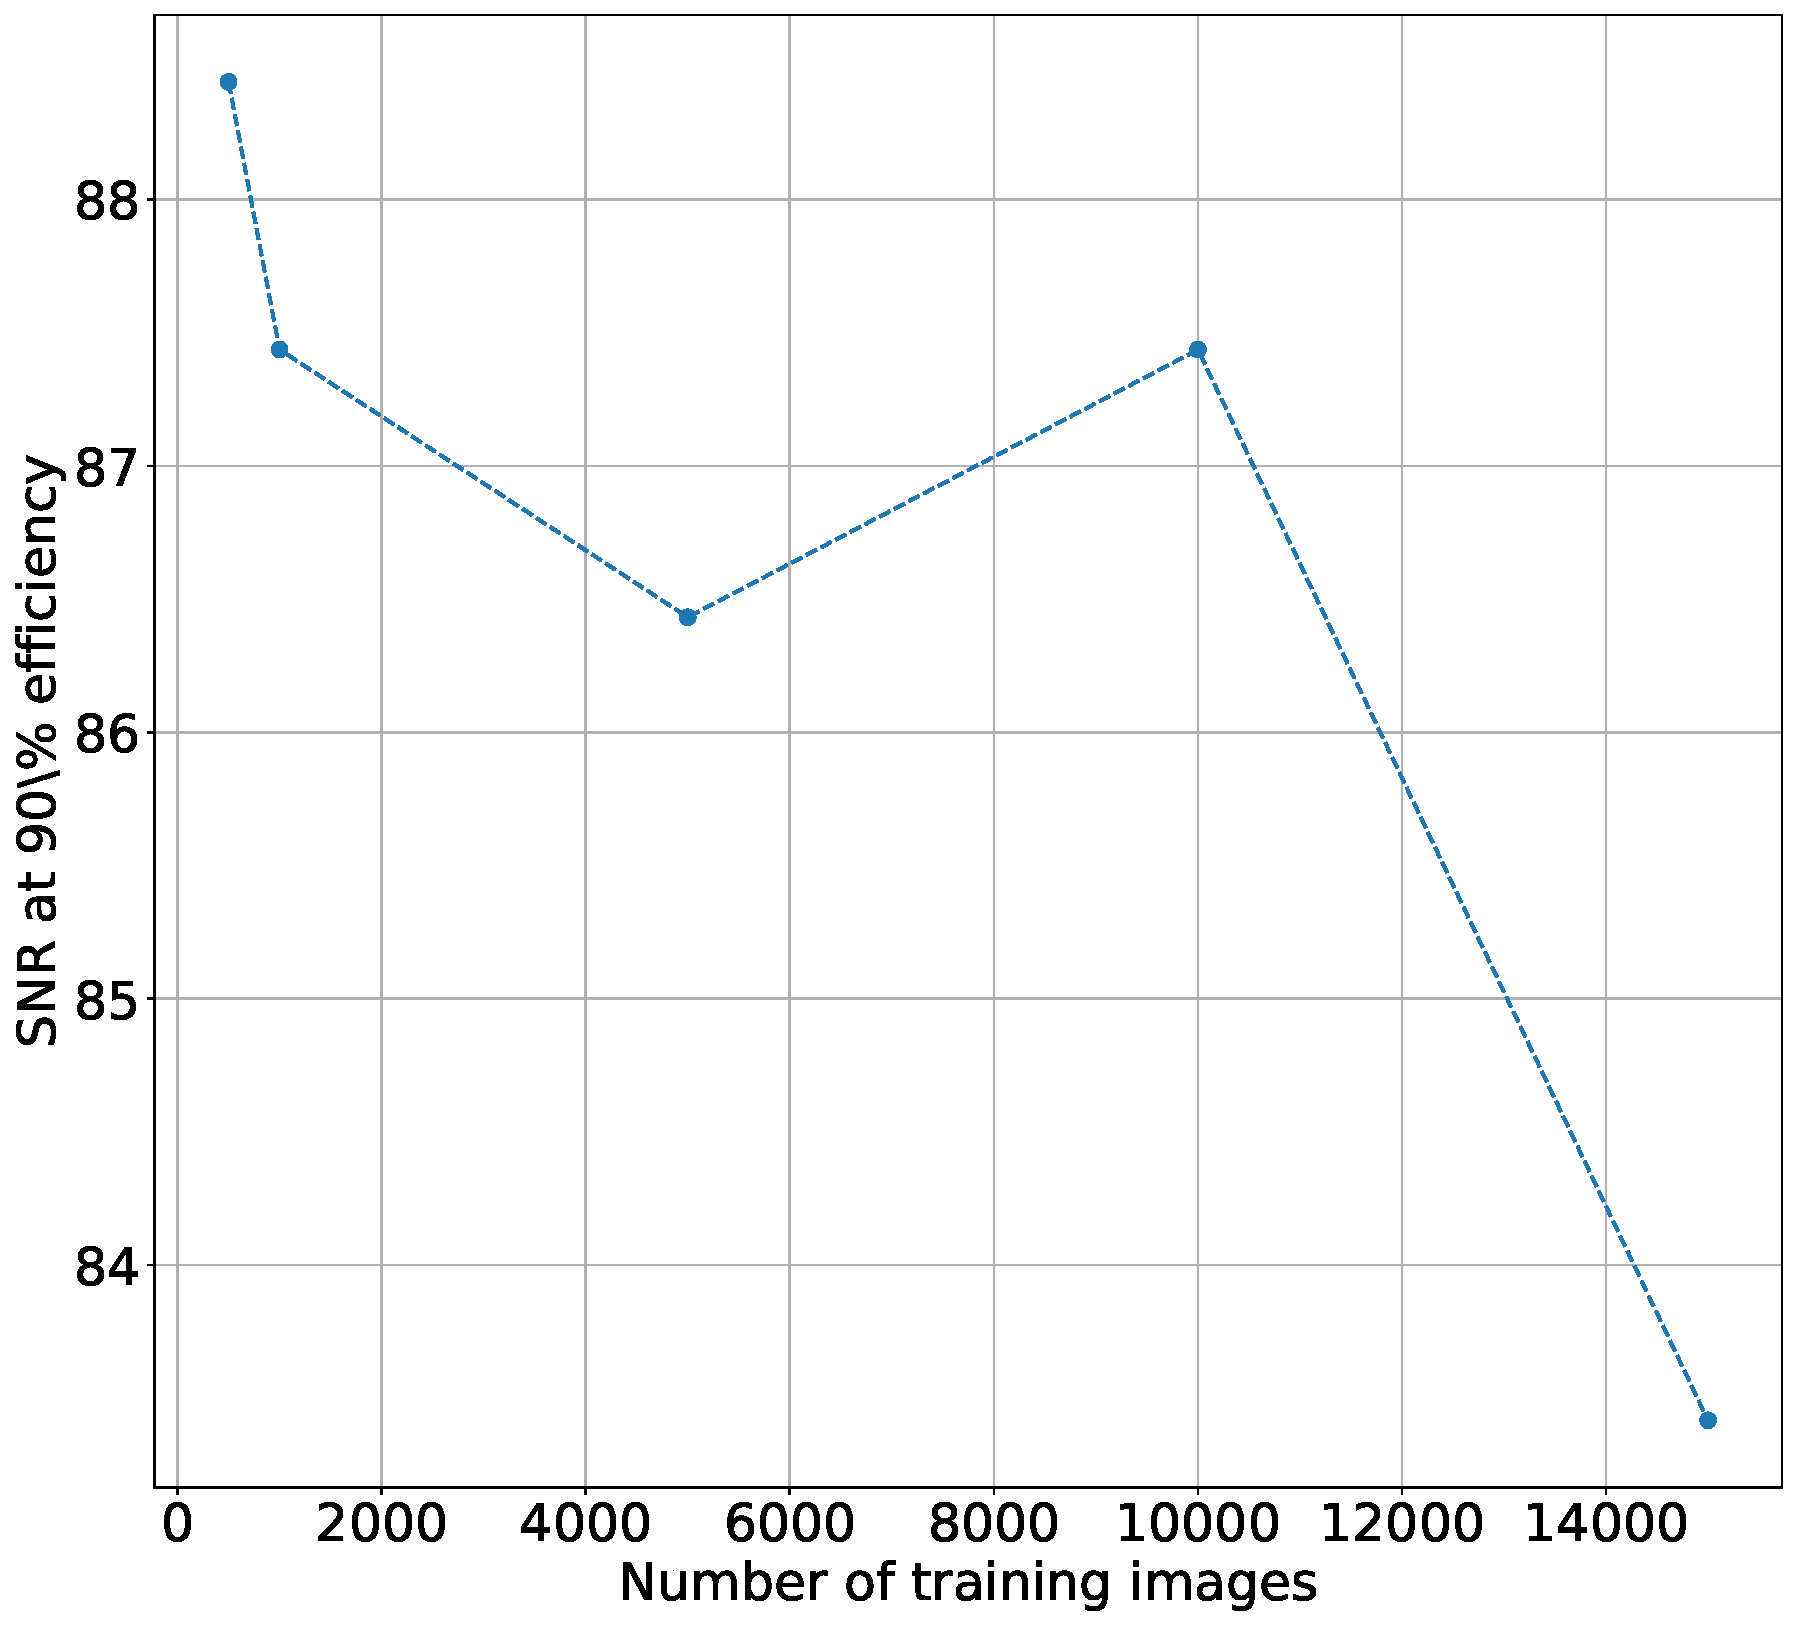
\includegraphics[width=\linewidth]{C4_cnn/gauss_sens_with_trainnum.pdf}
		\caption{}
		\label{machine:results:sens_size:gauss_sens:train}
	\end{subfigure}
	\caption[Sensitivity with size of data set for Gaussian noise simulations.]{The amount of training data needed for an \gls{CNN} to perform well depends on the problem. Here I show how the sensitivity changes as a function of the number of training examples for simulations in Gaussian noise. Figure \ref{machine:results:sens_size:gauss_sens:eff} shows the efficiency curves for each of the different data-set sizes and Fig.~\ref{machine:results:sens_size:gauss_sens:train} shows the values of \gls{SNR} at 90\% efficiency as the data size increases. This shows that the increase in data size causes a slight increase in the sensitivity of the search. The efficiency curve for 100 training examples is not shows in Fig.~\ref{machine:results:sens_size:gauss_sens:train} as it does not reach the 90\% efficiency mark.}
	\label{machine:results:sens_size:gauss_sens}
\end{figure}

When simulating signals in real O1 data, many of the sub-bands will contain instrumental lines. 
The noise class for the \gls{CNN} then contains many variations compared to the Gaussian noise case. 
This is a harder challenge for the \gls{CNN} as it increases the size of the parameter space.
Because of this, one would expect the network to need many more training examples to be able to achieve a similar sensitivity to Gaussian noise.
In Fig.~\ref{machine:results:sens_size:o1_sens:eff}, one can see that using 100 training examples is not enough for the \gls{CNN} to achieve any sensitivity at any \gls{SNR}. This means that the \gls{CNN} cannot classify any injection as detected using this number of training examples.
Figure \ref{machine:results:sens_size:o1_sens:train} seems to agree that real data poses a harder problem as the sensitivity drastically increases as the number of training examples is increased.
Therefore, more training examples are needed for the network to perform well on real data.

\begin{figure}[h]
	\begin{subfigure}[h]{0.5\textwidth}
		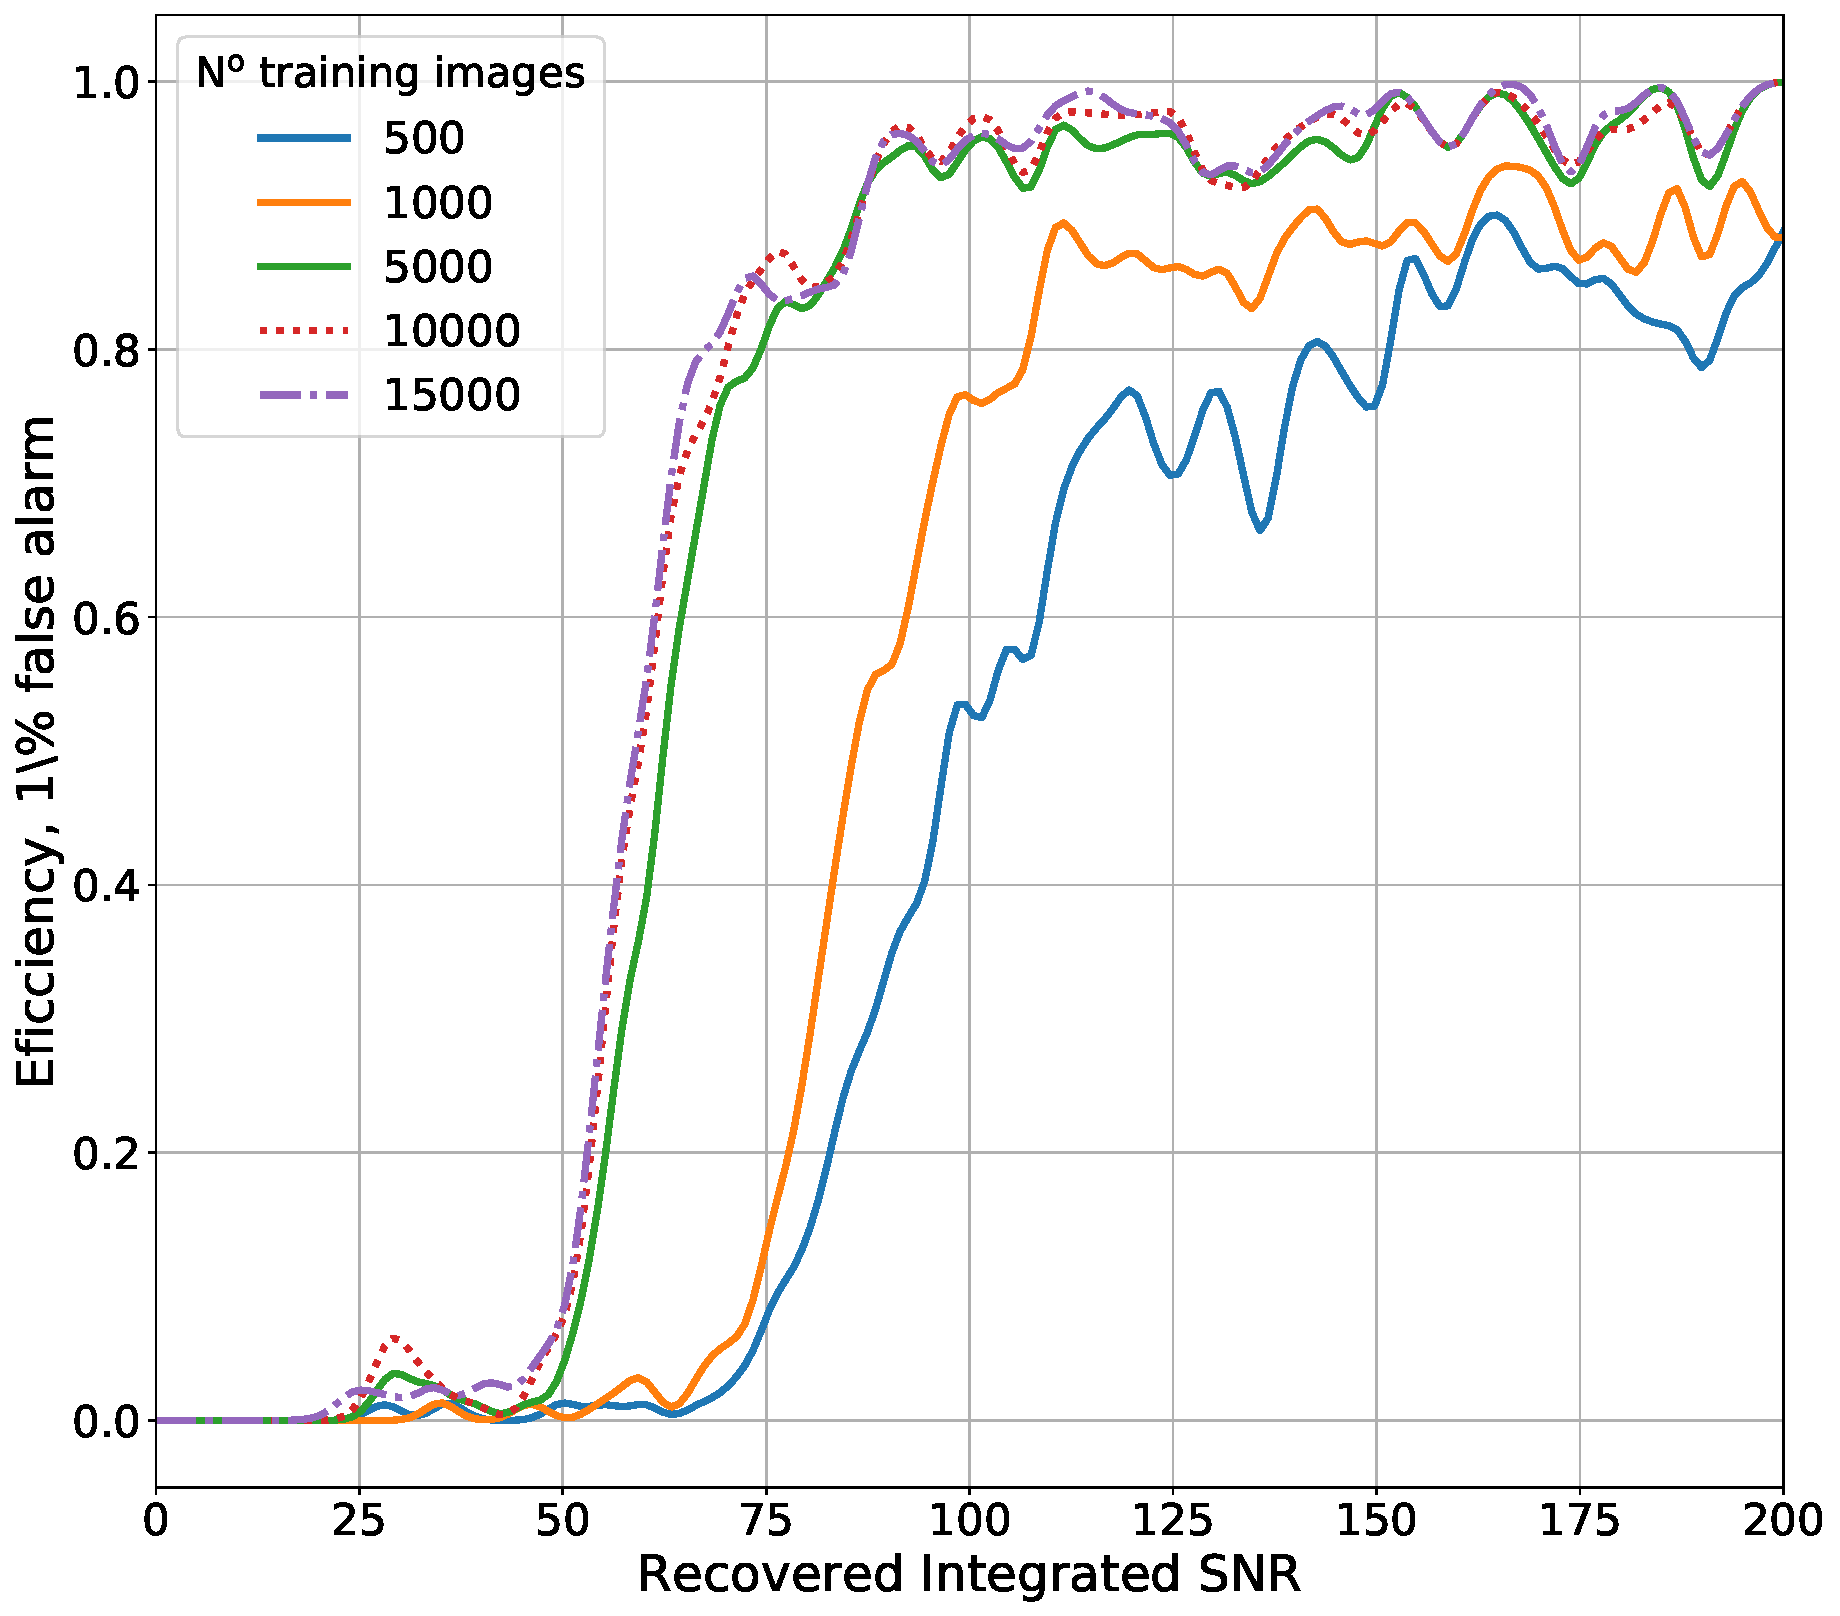
\includegraphics[width=\linewidth]{C4_cnn/o1_sens_with_trainnum_eff.pdf}
		\caption{}
		\label{machine:results:sens_size:o1_sens:eff}
	\end{subfigure}
	\begin{subfigure}[h]{0.5\textwidth}
		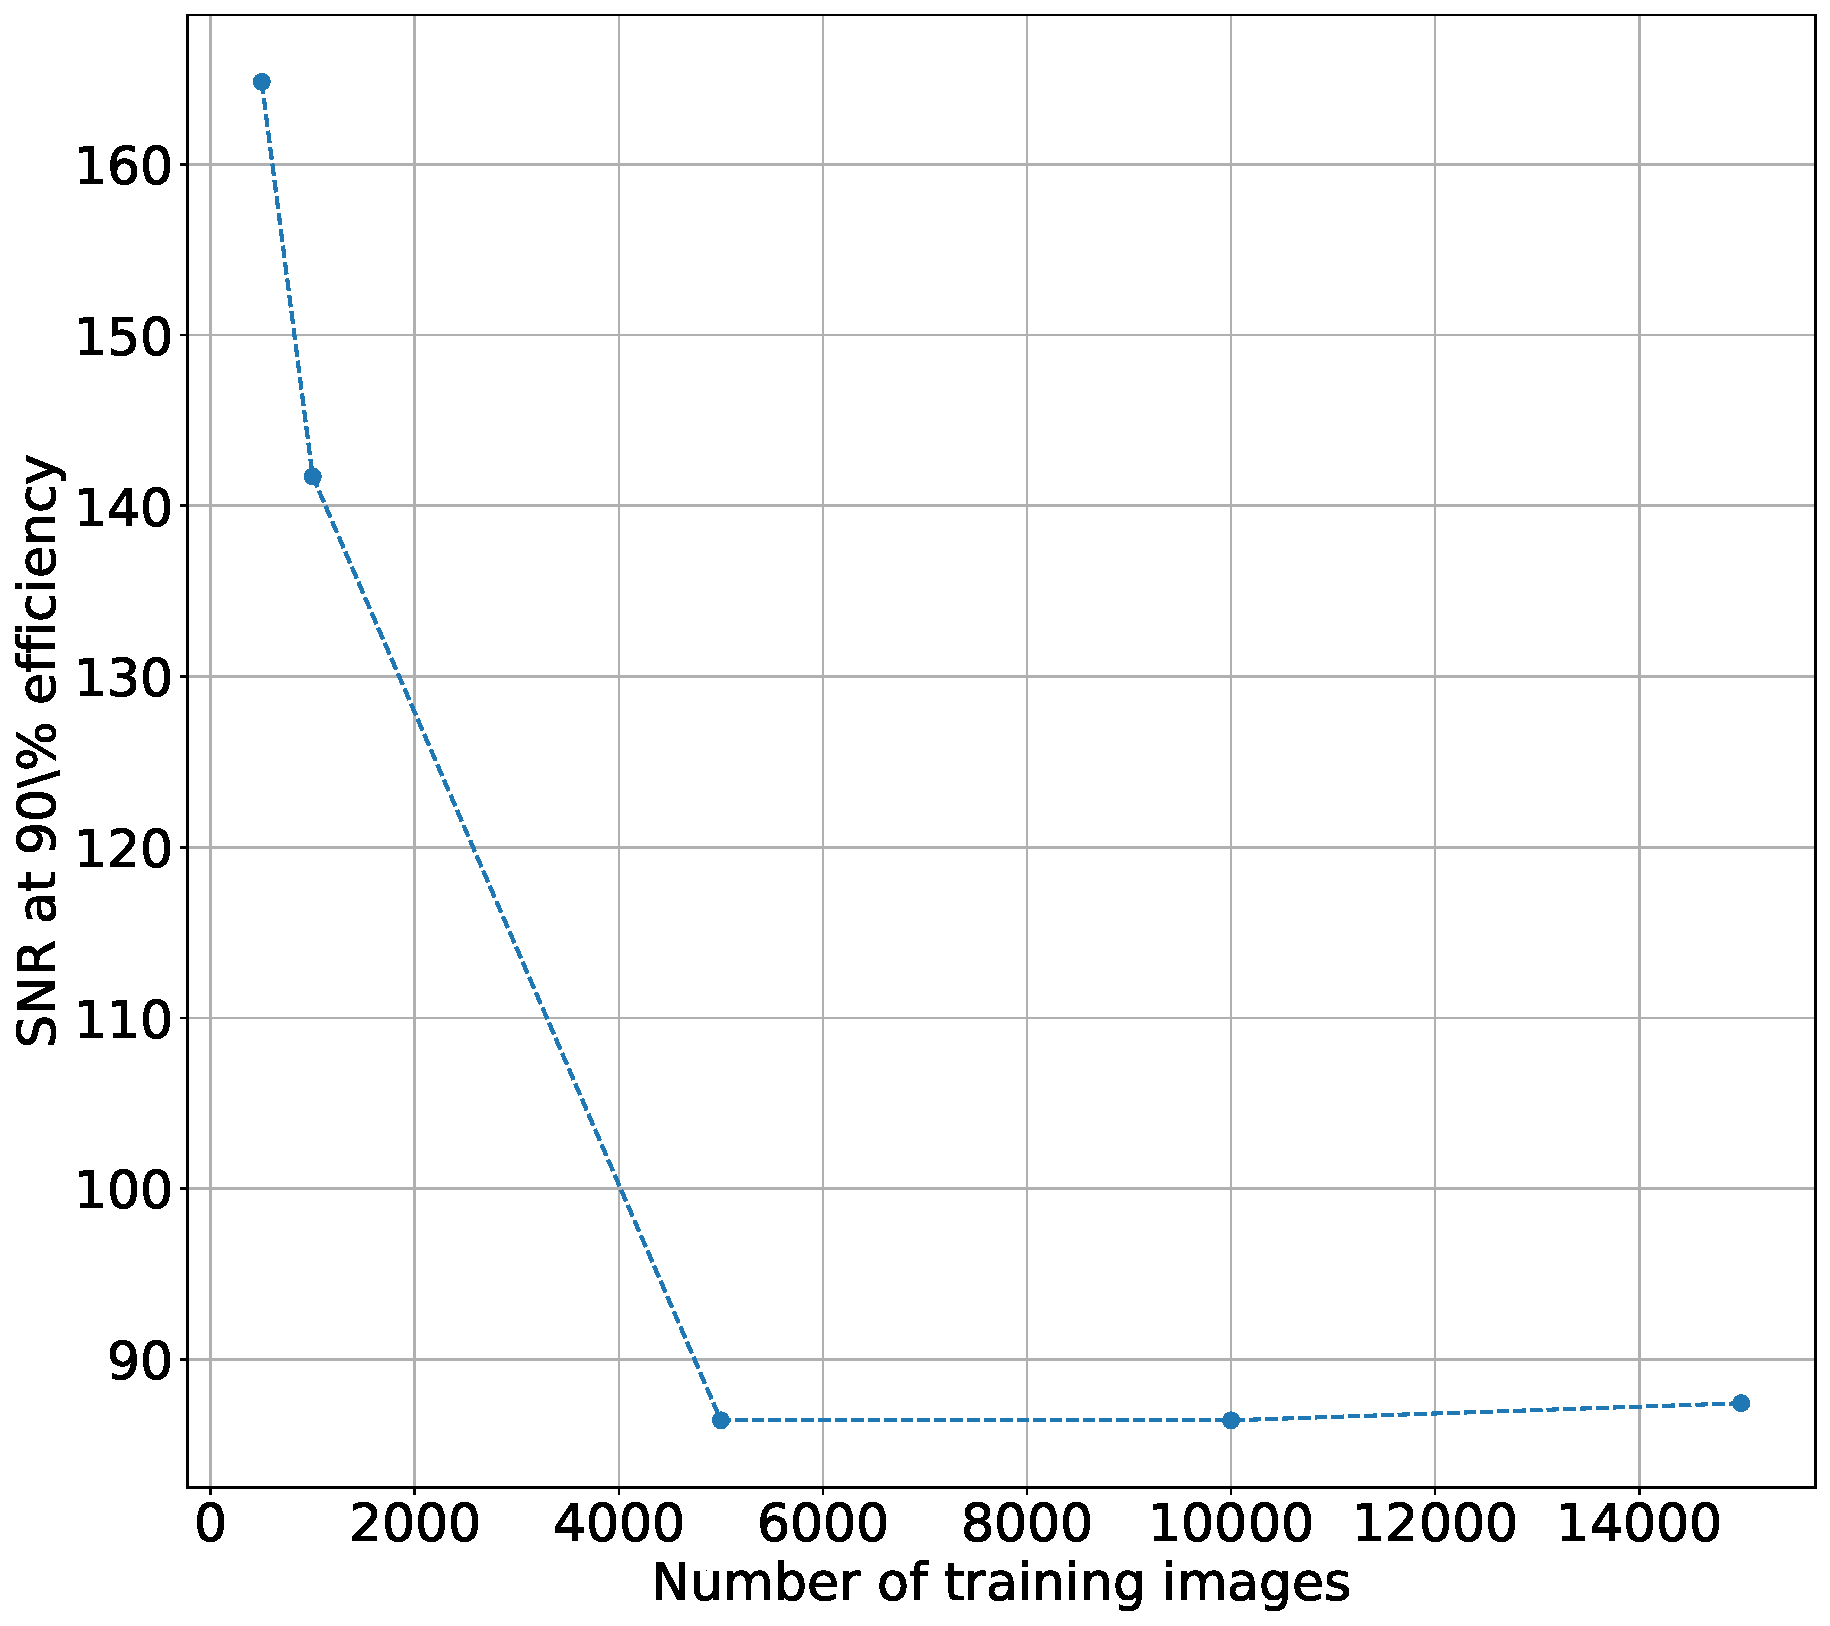
\includegraphics[width=\linewidth]{C4_cnn/o1_sens_with_trainnum.pdf}
		\caption{}
		\label{machine:results:sens_size:o1_sens:train}
	\end{subfigure}
	\caption[Sensitivity with size of data set for O1 simulations.]{Here I show how the sensitivity changes as a function of the number of training examples for simulations in O1 data. Figure \ref{machine:results:sens_size:o1_sens:eff} shows the efficiency curves for each of the different data-set sizes and Fig.~\ref{machine:results:sens_size:o1_sens:train} shows the values of \gls{SNR} at 90\% efficiency as the data size increases. This shows that the increase in data size causes a large increase in the sensitivity of the \gls{CNN}. The efficiency curve for 100 training examples is not shows in Fig.~\ref{machine:results:sens_size:o1_sens:train} as it does not reach the 90\% efficiency mark.}
	\label{machine:results:sens_size:o1_sens}
\end{figure}



%%%%%%%%%%%
%%%%%%%%%%%
\section{\label{cnn:networkvis}Network Visualisation}
%%%%%%%%%%%
%%%%%%%%%%%

Neural network are generally hard to visualise due to the large number or parameters in the network that have to be varied.
However, there are methods which can be used to see how input data is affected by the network.
This can be useful to see how the network performs when given certain types of data and gives some insight into how the networks work.

One way to visualise the network is to pass a piece of data through the network and see how each of the layers transforms the input.
Figs.~\ref{machine:cnn:vis:vitmap:signal}, \ref{machine:cnn:vis:vitmap:line} and \ref{machine:cnn:vis:vitmap:noise} show an example of this.
The layout is equivalent to that in Fig.~\ref{machine:results:cnnlayout}.
In these figures, the outputs from each of the layers in the \gls{CNN} are shown. The first being the convolutional layers, followed by their max-pooling layers. 
The final fully connected layers are illustrated with connecting lines.
The final neuron is then the value of the statistic which we use for the above analysis.
Fig.~\ref{machine:cnn:vis:vitmap:signal} shows an input of a Viterbi where the corresponding time-frequency spectrograms contained a strong \gls{CW} signal.
In this figure the next layer is the first convolutional layer, where 8 filtered Viterbi maps can be seen. 
This is then reduced in size by a max-pooling layer, followed by another convolutional and max-pooling layer.
After this point, the figures can be compared and it becomes obvious that different neurons light up when the input is part of the signal class or when it in the noise class.


\begin{figure}[h]
	\centering
	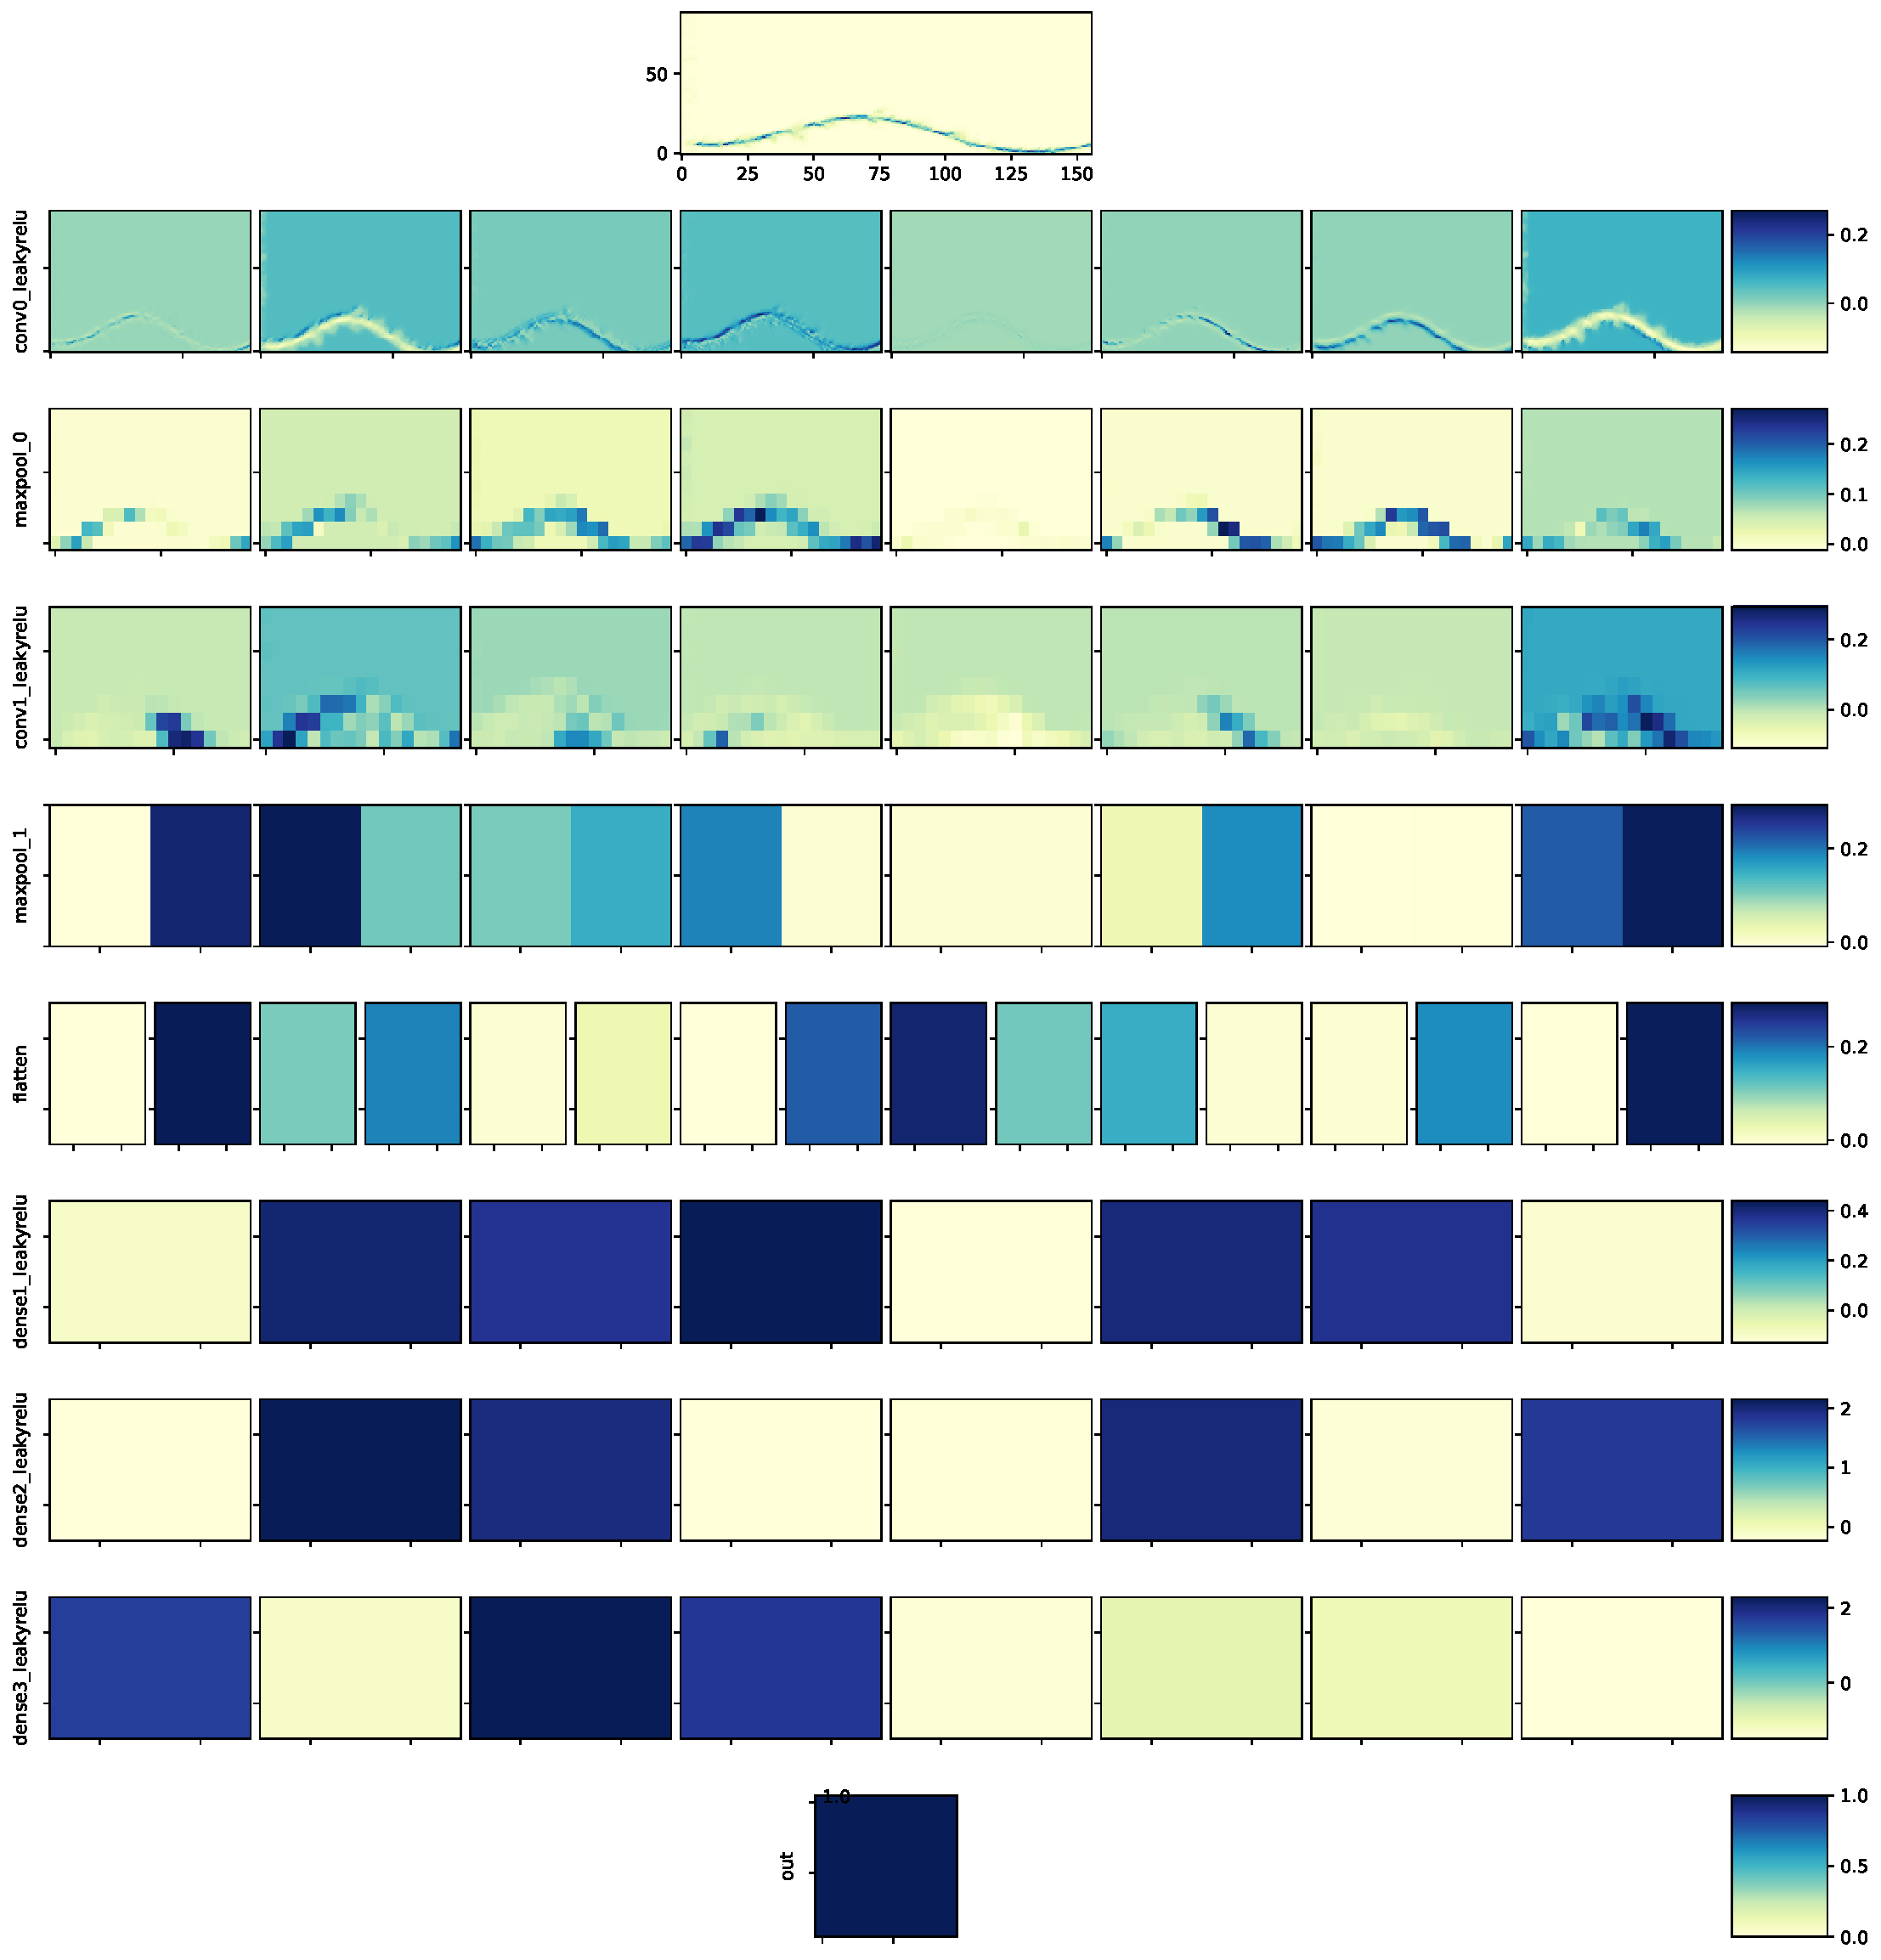
\includegraphics[width=\textwidth]{C4_cnn/vitmap_cnn_visualisation_signal.pdf}
	\caption[Network visualisation for a signal injection]{The \gls{CNN} can be visualised by seeing how a piece of data is passed through the network. This figure shows how the image is processed in each layer of the network. The input here is a Viterbi map which results from the SOAP algorithm. The input to SOAP here is a time-frequency spectrogram which contains a strong \gls{CW} signal. This then passes through 8 convolutional filters, then 8 max-pooling layers, then another set of 8 convolutional and max-pooling layers.the values are then flattened and it passes through 3 layers of 8 fully connected neurons.The final output neuron here is a 1 indicating that this is likely to contain a signal. }
	\label{machine:cnn:vis:vitmap:signal}
\end{figure}

\begin{figure}[h]
	\centering
	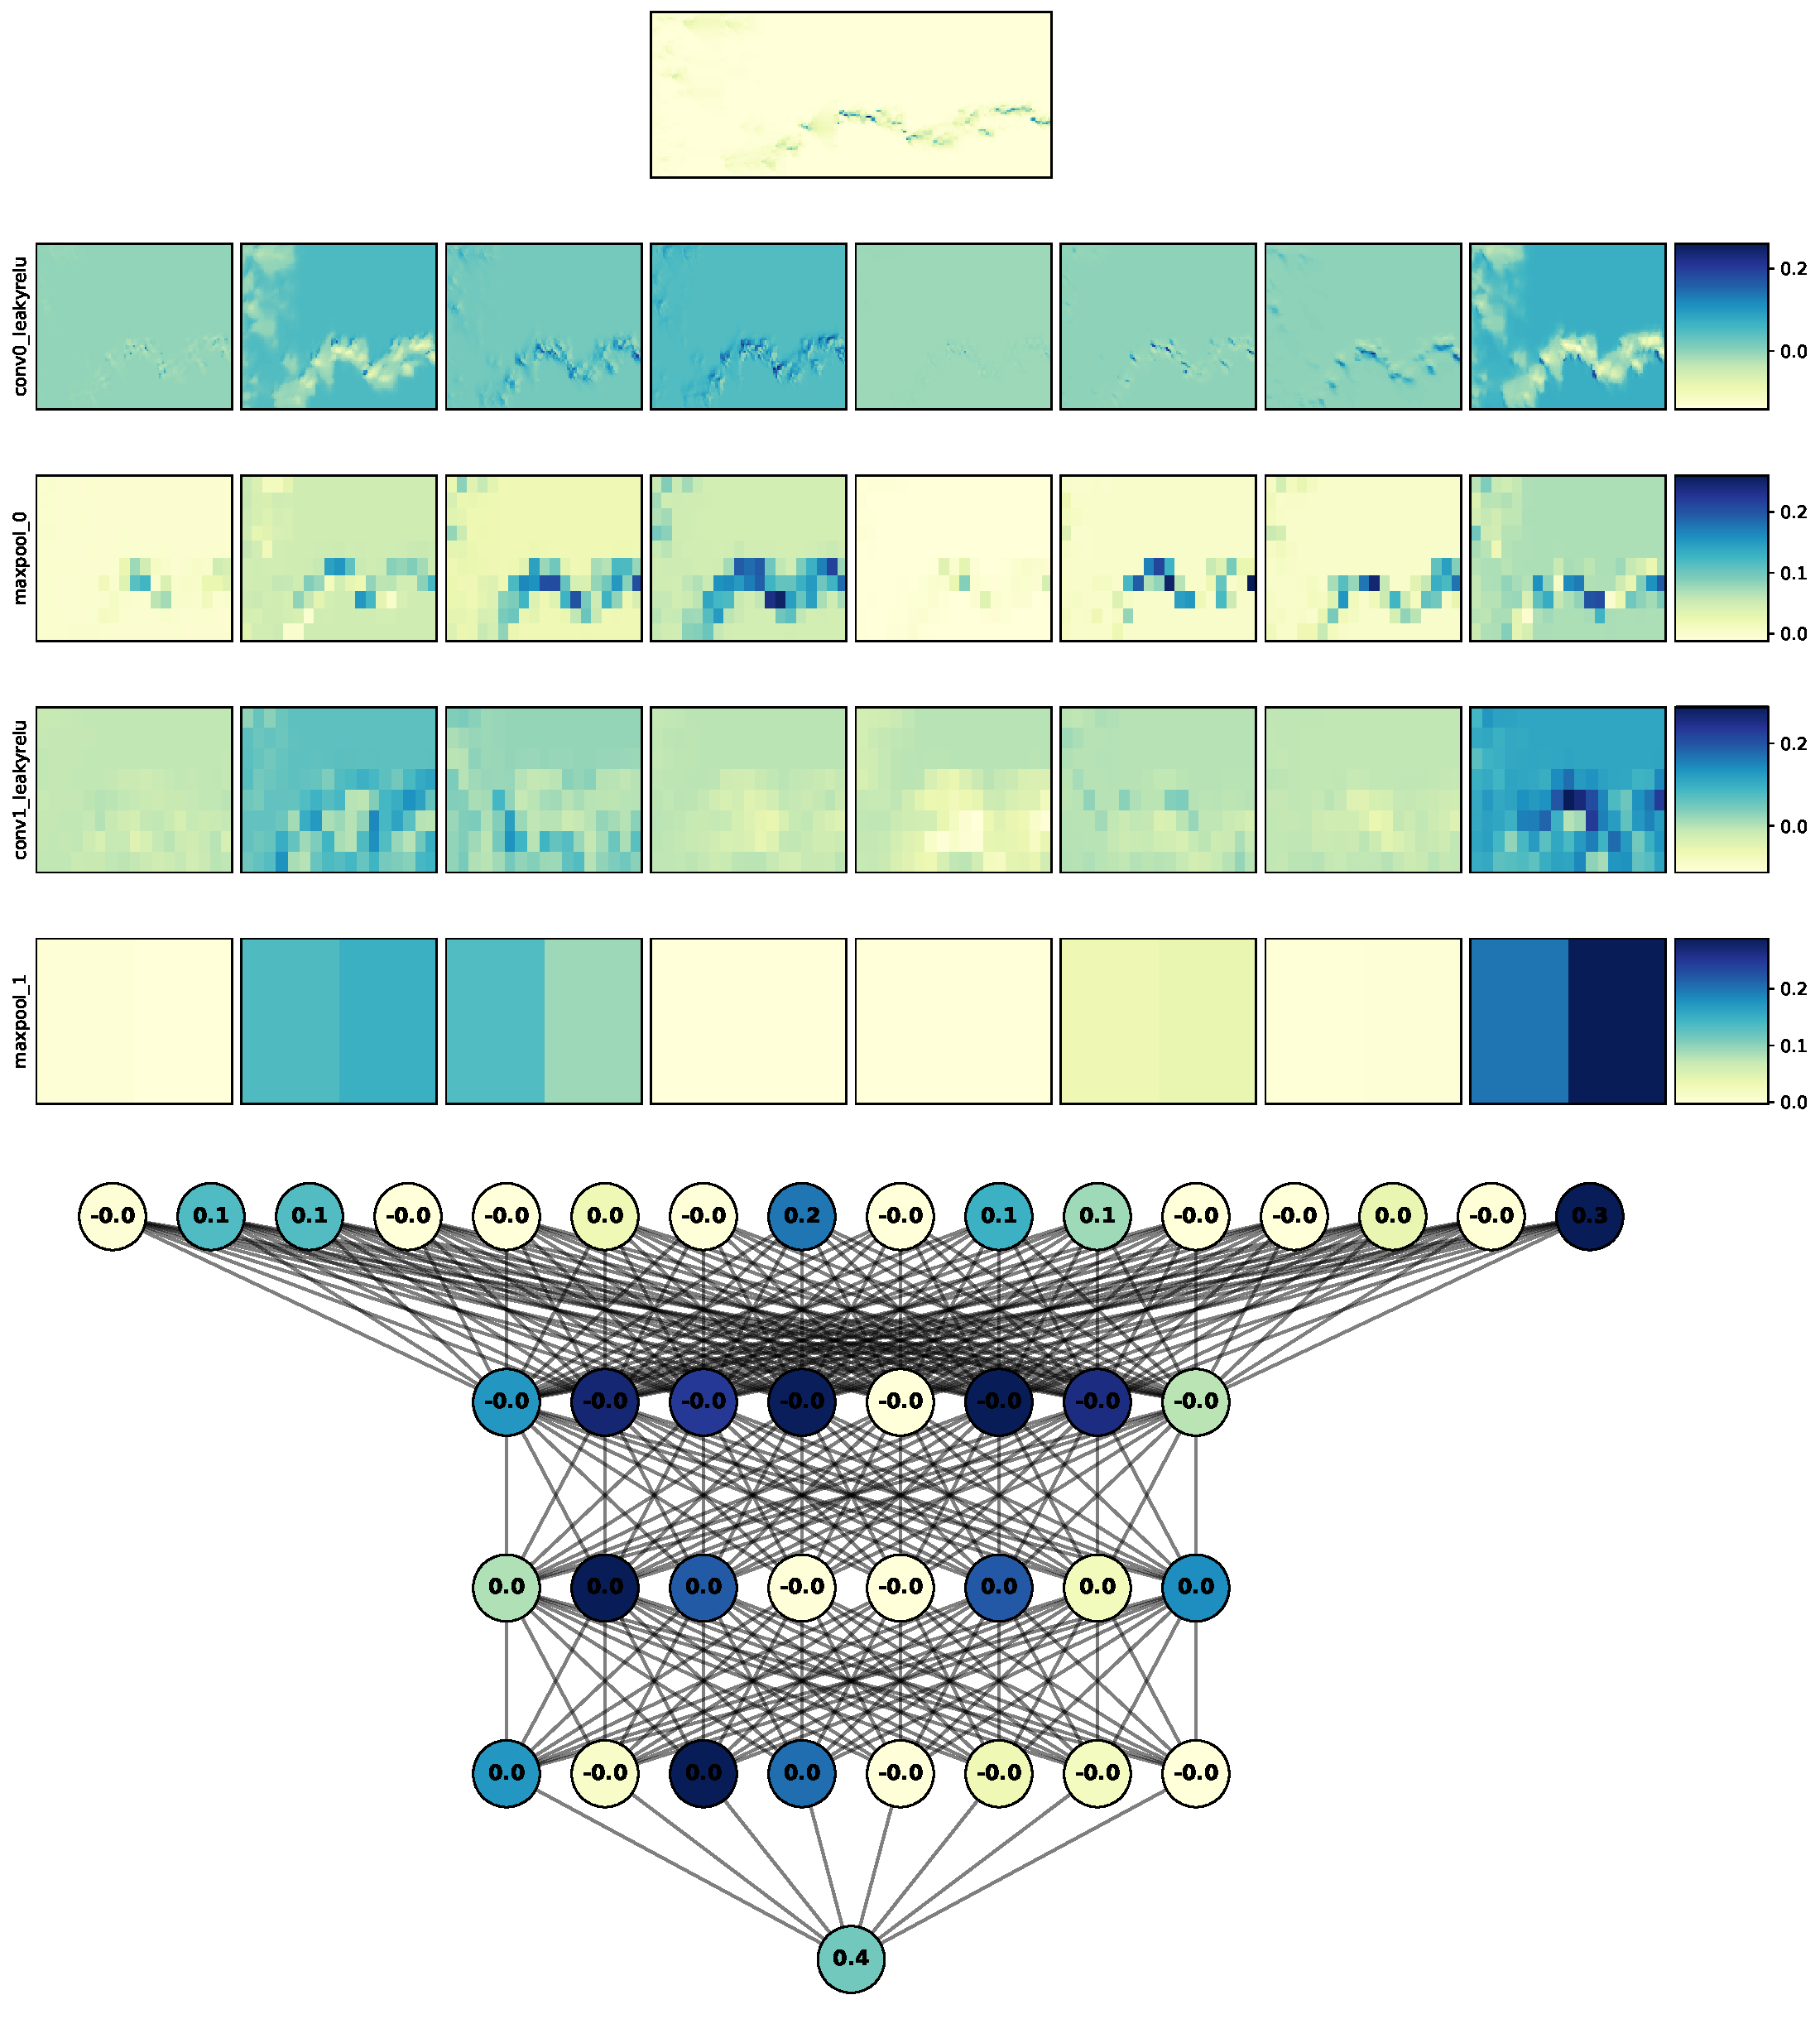
\includegraphics[width=\textwidth]{C4_cnn/vitmap_cnn_visualisation_line.pdf}
	\caption[Network visualisation for instrumental line.]{This visualisation of the Viterbi map \gls{CNN} shows the input of a Viterbi map where the time-frequency spectrogram contains an instrumental line. Here the output neuron has a value of 0.4, far below that in Fig.~\ref{machine:cnn:vis:vitmap:signal}.}
	\label{machine:cnn:vis:vitmap:line}
\end{figure}

\begin{figure}[h]
	\centering
	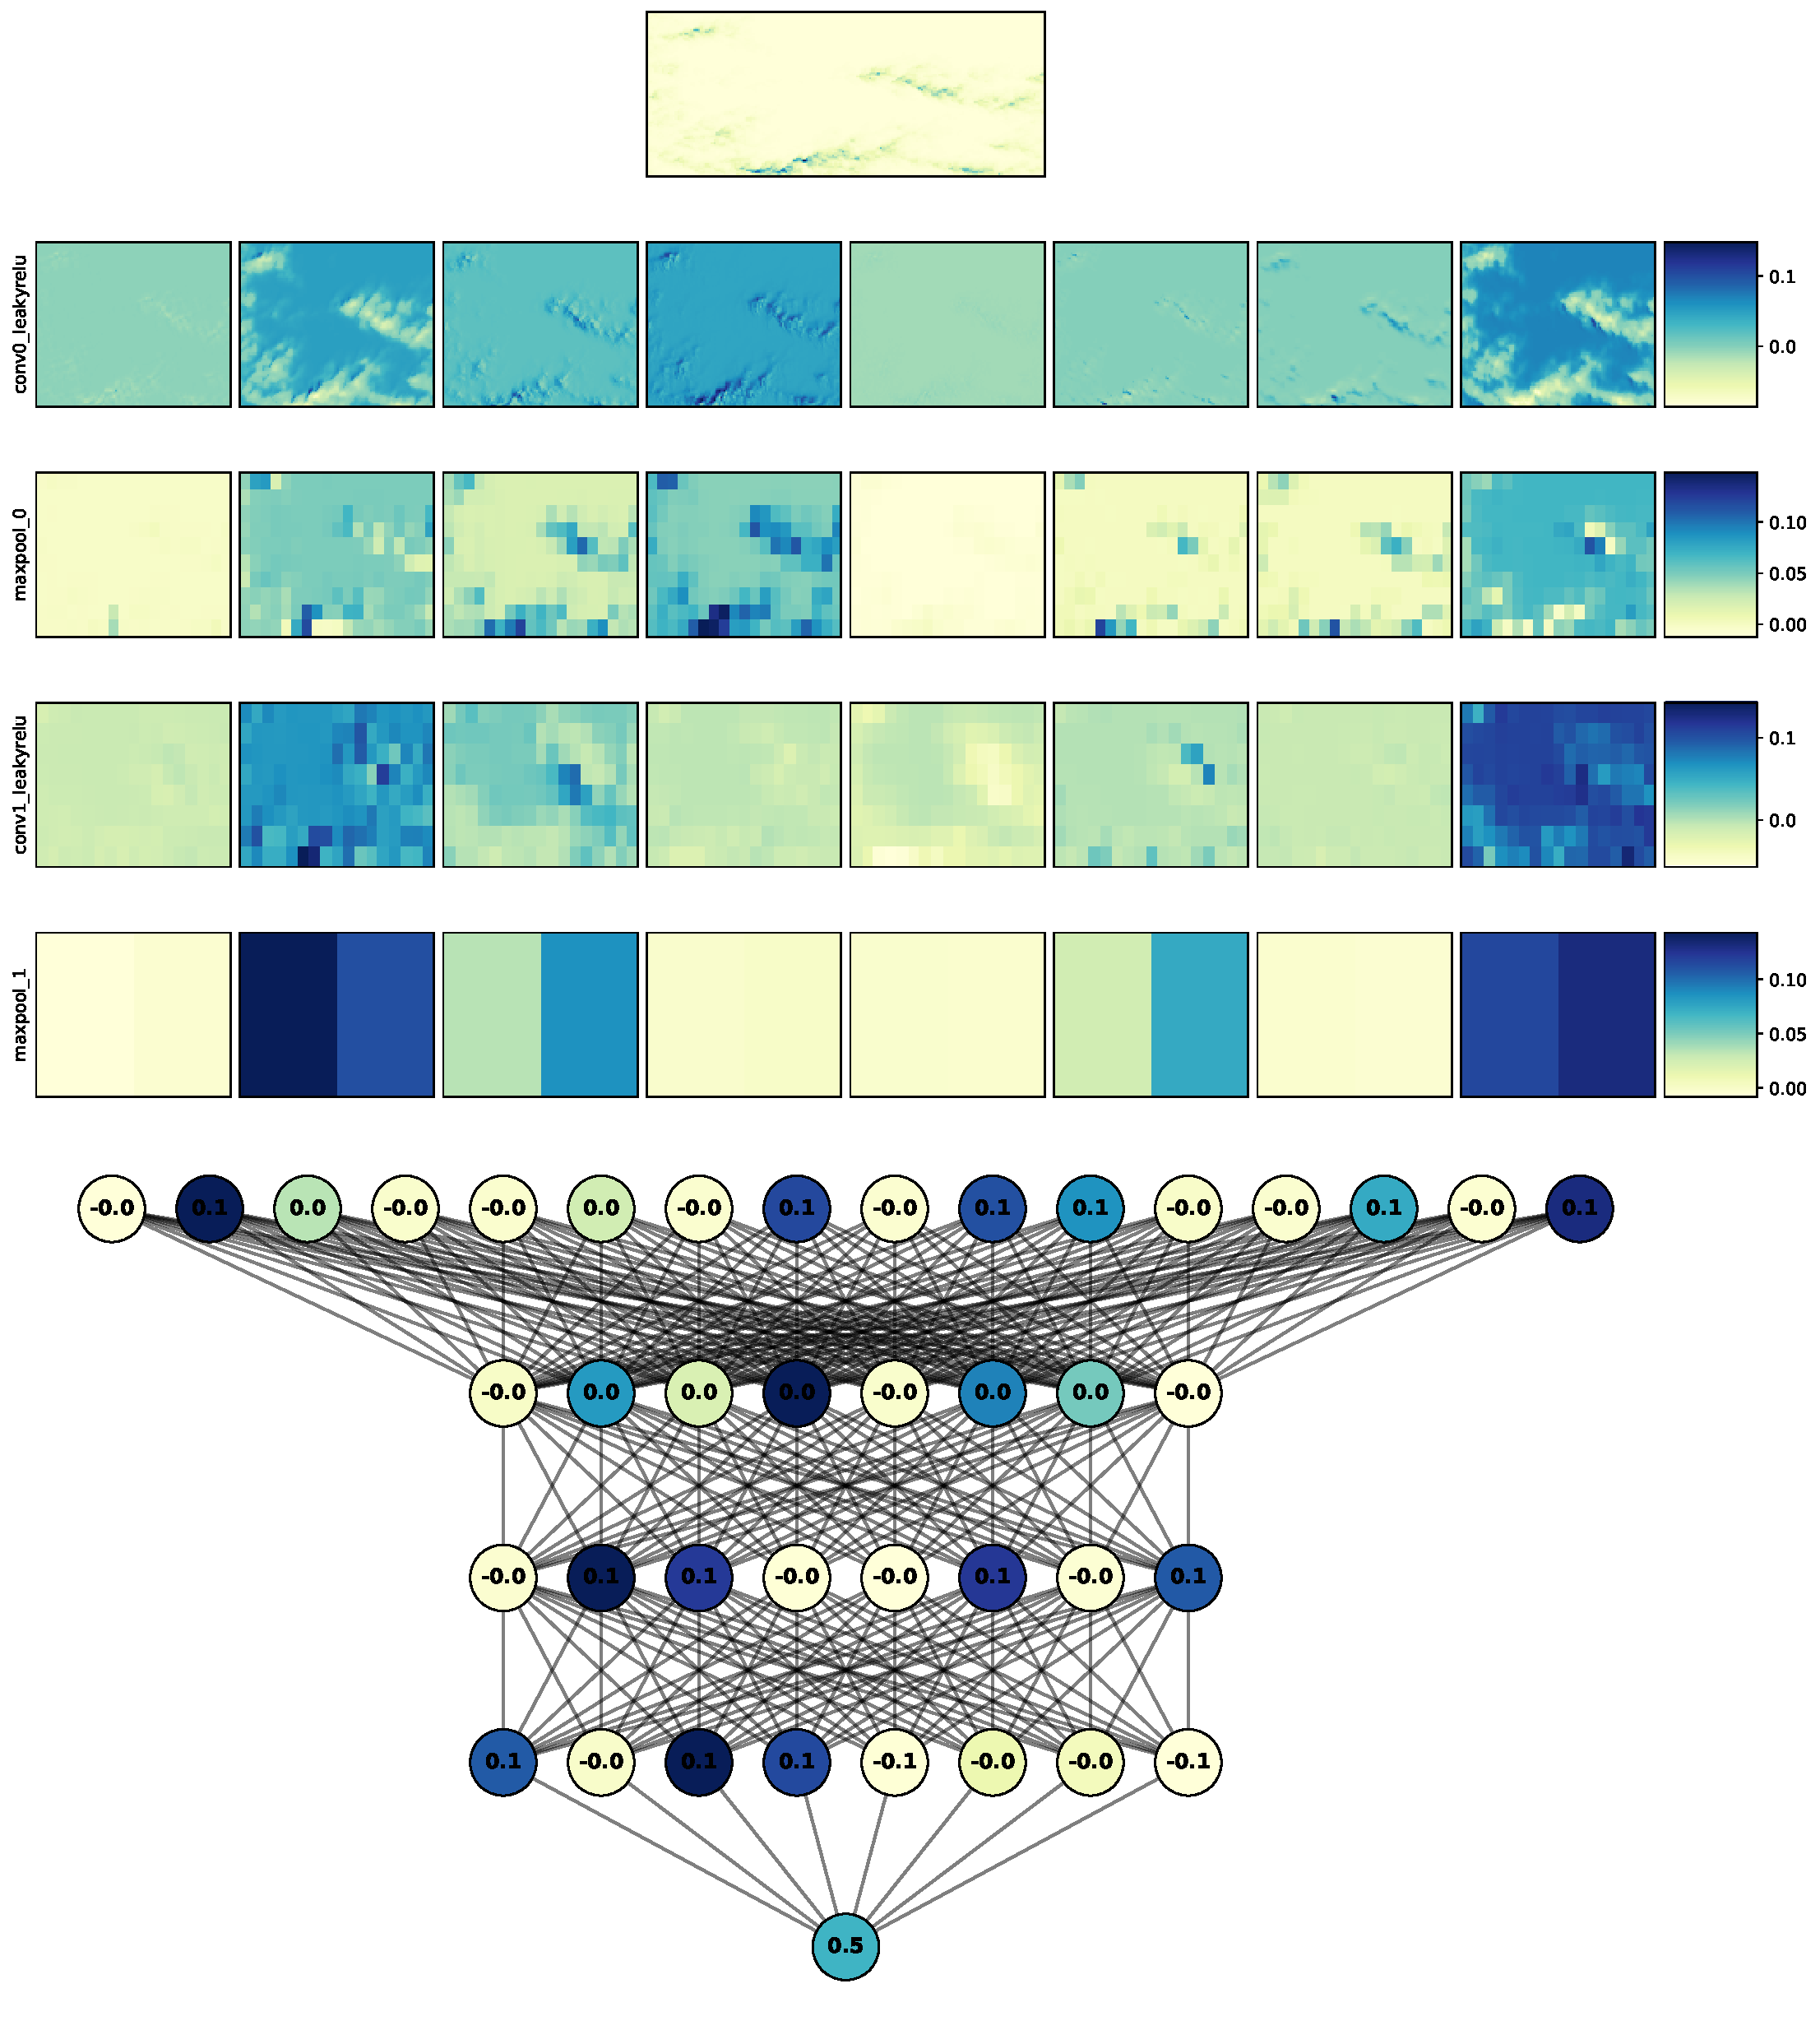
\includegraphics[width=\textwidth]{C4_cnn/vitmap_cnn_visualisation_noise.pdf}
	\caption[Network visualisation for noise.]{This visualisation of the Viterbi map \gls{CNN} shows the input of a Viterbi map where the time-frequency spectrogram contains just Gaussian noise. The output here is similar to the case where an instrumental line is injected, i.e. the output is much less than 1. }
	\label{machine:cnn:vis:vitmap:noise}
\end{figure}

\clearpage

%%%%%%%%%
%%%%%%%%
\section{Summary}
%%%%%%%%%
%%%%%%%%%


% main summary - what the paper was about
%
In this Chapter we summarise an extension of the SOAP algorithm \citep{bayley2019SOAPGeneralised}.
The extension makes use of a \gls{CNN} to limit the effect of
instrumental lines in a search for sources of \gls{CW}. 
The SOAP search has a number of outputs for a given input
spectrogram, in this paper we focus on using two of the outputs: the Viterbi statistic and the Viterbi map.
The Viterbi statistic has previously been used as a
measure of whether there is an astrophysical signal in a given frequency band as in \citep{bayley2019SOAPGeneralised}.
The Viterbi maps are output maps with the same shape as the input
spectrogram, these however give a value related to the probability that a signal is in any time-frequency bin. 
The aim of the \gls{CNN} approach is to use
both the Viterbi maps and spectrograms as input images to more effectively classify each
frequency band to either having an astrophysical signal or
not. This would then remove then need to manually look through frequency bands
and remove those which are contaminated with non-astrophysical (instrumental)
features. 

% technical results summary
%
We tested 6 separate \glspl{CNN} which take in some combination of the three representations of the input data: the Viterbi statistic, the Viterbi map and normalised spectrograms. 
The aim of using different input data types is that each would
provide a different representation of the same information, this had
the potential to increase the sensitivity of the search. The tests found
that the \gls{CNN} which uses the Viterbi map alone as input was more sensitive
than any other which used a single data type as input. Each of the \glspl{CNN}
that used a combination of input data types had a similar sensitivity to the
Viterbi map \gls{CNN}, therefore, we concluded that the Viterbi map provides the most
useful information when detecting a signal.  Given that the main aim of this
paper was to reduce the effect of instrumental lines on the SOAP search, in
Gaussian noise data (with no such lines), the \gls{CNN} search should achieve a
similar sensitivity to the Viterbi statistic alone. The tests in Gaussian noise
with S6 gaps showed that at a 95 \% efficiency and a 1\% false alarm rate the
Viterbi statistic and Viterbi map achieved a sensitivity of SNR 95 and 90
respectively. When the same test was run in real S6 data at a 95 \% efficiency
and a 1\% false alarm rate the Viterbi statistic and Viterbi map achieved
corresponding sensitivities of SNR 300 and 120 respectively. This demonstrates
that the Viterbi map approach has a much larger effect when used on real data
due to the presence of many instrumental lines. 

% comparison with other pipelines
%
These tests were once again repeated using a standard set of injections into S6
data such that a direct comparison can be made with other \gls{CW} search
pipelines. At a 95\% efficiency and a 1\% false alarm rate the Viterbi map
\gls{CNN} achieved a sensitivity of \gls{SNR} $ \sim 90$ and sensitivity depth
$\sim 14 \; \rm{Hz}^{-1/2}$ . We have shown that the SOAP + \gls{CNN} approach
can achieve a similar sensitivity to other semi-coherent \gls{CW} search
algorithms but with a greatly reduced computational cost.

% final statement
%
This search also offers a lot of flexibility in the signal type which can be
searched, in the above examples the focus is on isolated neutron stars such
that a comparison can be made to other \gls{CW} searches, however, this search
is un-modelled. By changing the input parameters of the search, different
signal types can be searched over, and in future work we aim to test its
ability to identify other sources of \gls{GW} such as neutron stars in binary systems.
Further to this, we aim to apply a more advances Bayesian analysis to enable parameter estimation of some parameters of the signal.
These parameters would then provide crucial information for a deeper followup by fully coherent pipelines. 





